%%%%%%%%%%%%%%%%%%%%%%%%%%%%%%%%%%%%%%%%%%%%%%%%%%%%%%%%%%%%%%%%%%%%%%%%%%%%%%%%%
%
% Purpose:  Top level document for \timeDesc.  DO NOT EDIT!!!
%
%
%
%%%%%%%%%%%%%%%%%%%%%%%%%%%%%%%%%%%%%%%%%%%%%%%%%%%%%%%%%%%%%%%%%%%%%%%%%%%%%%%%

\documentclass[twoside,11pt,titlepage]{report}

%
% Bring in the AMS math package
%
\usepackage{amsmath,amssymb,amsfonts,textcomp}

%
% Bring in the common page setup
%
\usepackage{dynenv}

%
% Bring in the model-specific commands
%
\usepackage{time}

%
% Bring in the graphics environment
%
\usepackage{graphicx}

%
% Bring in the hyper ref environment
%
\usepackage[colorlinks,plainpages=false]{hyperref}
%  keywords for pdfkeywords are separated by commas
\hypersetup{
   pdftitle={\timeDesc},
   pdfauthor={\ModelAuthor},
   pdfkeywords={\ModelKeywords},
   pdfsubject={\timeDesc}}

\begin{document}

%%%%%%%%%%%%%%%%%%%%%%%%%%%%%%%%%%%
% Front matter
%%%%%%%%%%%%%%%%%%%%%%%%%%%%%%%%%%%
\pagenumbering{roman}

\docid{models/environment/time}
\docrev{1.2.2}
\date{\RELEASEMONTH\ \RELEASEYEAR}
\modelname{\timeDesc}
\doctype{}
\author{\ModelAuthor}
\managers{
  Robert O. Shelton \\ Project Manager \\
  Michael T. Red \\ Simulation and Graphics Branch Chief \\
  R. Matt Ondler \\ Software, Robotics, and Simulation Division Chief}
\pdfbookmark{Title Page}{titlepage}
\makeDynenvTitlepage

\pdfbookmark{Abstract}{abstract}
%%%%%%%%%%%%%%%%%%%%%%%%%%%%%%%%%%%%%%%%%%%%%%%%%%%%%%%%%%%%%%%%%%%%%%%%%%%%%%%%%
%
% Purpose:  Abstract for the time model
%
% 
%
%%%%%%%%%%%%%%%%%%%%%%%%%%%%%%%%%%%%%%%%%%%%%%%%%%%%%%%%%%%%%%%%%%%%%%%%%%%%%%%%


\begin{abstract}

% insert text
% This file was converted to LaTeX by Writer2LaTeX ver. 1.0 beta3
% see http://writer2latex.sourceforge.net for more info
The \timeDesc\ in \JEODid\ represents a 
complete reformulation from the UTIME structure seen in JEOD1.x.  Like 
its predecessor, it is responsible for tracking time as a simulation 
advances; unlike its predecessor, it can do so in any number of time 
representations, using any number of clocks, that may be ticking at 
different rates from one another.

The \timeDesc\ accurately represents
the most commonly used reference times throughout a simulation, and
includes the capacity to control additional user-specified time
references.


\end{abstract}


\pdfbookmark{Contents}{contents}
\tableofcontents
\vfill

\pagebreak

%%%%%%%%%%%%%%%%%%%%%%%%%%%%%%%%%%%
% Main Document Body
%%%%%%%%%%%%%%%%%%%%%%%%%%%%%%%%%%%
\pagenumbering{arabic}


\setcounter{chapter}{0}

%----------------------------------
\chapter{Introduction}\hyperdef{part}{intro}{}\label{ch:intro}
%----------------------------------

\section{Purpose and Objectives of the \timeDesc}
%%%%%%%%%%%%%%%%%%%%%%%%%%%%%%%%%%%%%%%%%%%%%%%%%%%%%%%%%%%%%%%%%%%%%%%%%%%%%%%%%
%
% Purpose:  Introduction for the time model.
%
% 
%
%%%%%%%%%%%%%%%%%%%%%%%%%%%%%%%%%%%%%%%%%%%%%%%%%%%%%%%%%%%%%%%%%%%%%%%%%%%%%%%%
%\section{Purpose and Objectives of \timeDesc}
% Incorporate the intro paragraph that used to begin this Chapter here. 
% This is location of the true introduction where you explain what this model 
% does.
% This file was converted to LaTeX by Writer2LaTeX ver. 1.0 beta3
% see http://writer2latex.sourceforge.net for more info
The \timeDesc\ in \JEODid\ represents a
complete reformulation from the UTIME structure seen in JEOD1.x.  Like
its predecessor, it is responsible for tracking time as a simulation
advances; unlike its predecessor, it can do so in any number of time 
representations, using any number of clocks, that may be ticking at
different rates from one another.


While the SI second is a well-defined quantity, counted to high 
precision by atomic clocks, and incorporated into many physical
constants, it is not always the best clock to use for modeling
purposes.  For example, when modeling the rotation of Earth, it is
preferable to use a sidereal clock (1 day = 1 rotation), rather than
the synodic clock (1 day = 1 solar passage) associated with the SI
second.  The length of the SI second was chosen such that there would
be approximately 86,400 seconds in one synodic day, and the passage of
the SI second is represented by International Atomic Time (TAI).
 However, the length of the synodic day, now associated with Universal
Time (UT1), rarely lasts 86,400 SI seconds, and fluctuates with little
predictability.  Earth-based civil-time, or Universal Coordinated
Time (UTC), attempts to closely match the passage of UT1, while ticking 
at the same rate as TAI.  


Further complicating the management of time are other clocks with
various epochs (points in time where their value was 0). 
 Mission-Elapsed-Time (MET) is often used to track time since a 
mission began, and the Global Positioning System (GPS) has its own clock.
Users may wish to run only in local time, rather than UTC, or 
have clocks that can output their data in two or more local times for
international missions.

In JEOD 1.x, there was a tacit assumption that time always advanced
forward.  In this implementation, we can run time in reverse to find,
for example, a set of initial conditions that produce a desired
end-state.  As we look toward making JEOD applicable to
interplanetary missions, it may be desirable to incorporate a
solar-based timescale, with capability for relativistic corrections;
that capability has also been implemented.














\section{Context within JEOD}
The following document is parent to this document:
\begin{itemize}
\item{\href{file:\JEODHOME/docs/JEOD.pdf}
           {\em JSC Engineering Orbital Dynamics}}
			  \cite{dynenv:JEOD}
\end{itemize}

The \timeDesc\ forms a component of the \ModelClass\ suite of
models within \JEODid. It is located at
models/\ModelClass/time.

\section{Documentation History}
%%%%%%%%%%%%%%%%%%%%%%%%%%%%%%%%%%%%%%%%%%%%%%%%%%%%%%%%%%%%%%%%%%%%%%%%%%%%%%%%%
%
% Purpose:  Change history for document for the time model
%
% 
%
%%%%%%%%%%%%%%%%%%%%%%%%%%%%%%%%%%%%%%%%%%%%%%%%%%%%%%%%%%%%%%%%%%%%%%%%%%%%%%%%


%\section{Documentation History}
%%% Status of this and only this document.  Any date should be
%relevant to when 
%%% this document was last updated and mention the reason (release,
%bug fix, etc.)
%%% Mention previous history aka JEOD 1.4-5 heritage in this section.

\begin{tabular}{||l|l|l|l|} \hline
 {\bf Author} & {\bf Date} &  {\bf Revision} & {\bf Description} \\ \hline \hline
 Gary Turner    & November 2009 & 1.0  & JEOD 2.0.0 release \\ \hline
 Gary Turner,   &             &       & JEOD 2.0.1 release \\ 
 Blair Thompson & March 2010 & 1.1 & Addition of clarifying text \\
                &             &       &   New instructions for obtaining default data \\ \hline
  Gary Turner   & April 2011  & 1.2 & Addition of comments regarding TimeStandard \\ 
     &      &     & and edits for change from Time to JeodBaseTime  \\ \hline
  Gary Turner   & January 2012  & 1.2.1 & Addition of comments regarding Julian \\ 
     &      &     & Date inclusion for release 2.2.  \\ \hline
  Gary Turner   & January 2014  & 1.2.2 & Addition of comments regarding initialization \\
     &      &     & and setting epochs for UDEs   \\ \hline
  Gary Turner   & January 2014  & 1.3 & Addition of comments regarding lead seconds \\ \hline
\end{tabular}



\section{Documentation Organization}
This document is formatted in accordance with the
NASA Software Engineering Requirements Standard~\cite{NASA:SWE}
and is organized into the following chapters:

\begin{description}
%% longer chapter descriptions, more information.

\item[Chapter 1: Introduction] --
This introduction contains four sections: purpose and objective,
context within JEOD, document history, and document organization.

\item[Chapter 2: Product Requirements] --
Describes requirements for the \timeDesc.

\item[Chapter 3: Product Specification] --
Describes the underlying theory, architecture, and design of the
\timeDesc\ in detail.  It will be organized in
four sections: Conceptual Design, Mathematical Formulations, Detailed
Design, and Version Inventory.

\item[Chapter 4:  User Guide] --
Describes how to use the \timeDesc\ in a Trick simulation.  It
is broken into three sections to represent the JEOD
defined user types; Analysts or users of simulations (Analysis),
Integrators or developers of simulations (Integration),
and Model Extenders (Extension).

\item[Chapter 5: Verification and Validation] --
Contains \timeDesc\ verification and validation procedures and
results.

\end{description}



\chapter{Product Requirements}\hyperdef{part}{reqt}{}\label{ch:reqt}
%----------------------------------
\requirement{Top-level requirement}
\label{reqt:toplevel}
\begin{description}
\item[Requirement:]\ \newline
  This model shall meet the JEOD project requirements specified in
  the \JEODid\
  \hyperref{file:\JEODHOME/docs/JEOD.pdf}{part1}{reqt}{ top-level
  document}.
\item[Rationale:]\ \newline
  This model shall, at a minimum,  meet all external and internal requirements
  applied to the \JEODid\ release.
\item[Verification:]\ \newline
     Inspection \vref{inspect:TLI}.
\end{description}


%%%%%%%%%%%%%%%%%%%%%%%%%%%%%%%%%%%%%%%%%%%%%%%%%%%%%%%%%%%%%%%%%%%%%%%%%%%%%%%%%
%
% Purpose:  requirements for the time model
%
% 
%
%%%%%%%%%%%%%%%%%%%%%%%%%%%%%%%%%%%%%%%%%%%%%%%%%%%%%%%%%%%%%%%%%%%%%%%%%%%%%%%%

% add text here to describe general model requirements
% text is of the form:
%\requirement{REQUIREMENT DESCRIPTION}
%\label{reqt:REQT_DESC_ABBREVIATED}
%\begin{description}
%  \item[Requirement:]\ \newline
%     <Insert description of requirement> 
%  \item[Rationale:]\ \newline
%     <Insert description of rationale> 
%  \item[Verification:]\ \newline
%     <Insert description of verification (e.g. "Inspection")> 
%\end{description}

\requirement{Physical Time}
\label{reqt:physicaltime}
\begin{description}
\item[Requirement:]\ \newline
The \timeDesc\ shall include a representation of time that can be used for 
integration of the dynamic vehicle state.  It shall be capable of propagating 
forward, and in reverse.
\item[Rationale:]\ \newline
Not all time representations accurately represent the standard definition of 
``second'', which is required for the integration of the physical state.  There 
should be one clearly identified representation that is always used for 
integration purposes.  
To identify a suitable state that is capable of creating a particular outcome, 
it is necessary to be able to integrate from the outcome back in time to the 
original state.

\item[Verification:]\ \newline
Test \vref{test:1dynonly}, test \vref{test:sim2scalefactor}, and test 
\vref{test:timereversal}.
\end{description}

\requirement{Necessary Clocks}
\label{reqt:datatimerepresentation}
\begin{description}
  \item[Requirement:]\ \newline
    The \timeDesc\ shall be able to represent time in
    each of the following time systems:

    \subrequirement{TAI}\label{reqt:data_time_rep_TAI}
      \ \newline
      International Atomic Time,
      a very accurate and stable time scale calculated as a weighted 
      average of the time kept by about 200 cesium atomic clocks in 
      over 50 national laboratories worldwide.

    \subrequirement{UT1}\label{reqt:data_time_rep_UT1}
      \ \newline
      Universal Time, a measure of the rotation angle of the Earth 
      as observed astronomically.

    \subrequirement{UTC}\label{reqt:data_time_rep_UTC}
      \ \newline
      Coordinated Universal Time, the basis for the worldwide system 
      of civil time.

    \subrequirement{MET}\label{reqt:data_time_rep_MET}
      \ \newline
      Any number of Mission Elapsed Times, each with distinct user-defined 
      epochs.

    \subrequirement{GPS}\label{reqt:data_time_rep_GPS}
      \ \newline
      The time system used by the Global Positioning System.
		
    \subrequirement{TT}\label{reqt:data_time_rep_TT}
      \ \newline
      Terrestrial Time, the time system used by the Ephemeris models.
		
    \subrequirement{GMST}\label{reqt:data_time_rep_GMST}
      \ \newline
      Greenwich Mean Sidereal Time, the time system used to simulate the
			rotation of Earth.
		
    \subrequirement{TDB}\label{reqt:data_time_rep_TDB}
      \ \newline
      Barycentric Dynamic Time, potentially useful for higher fidelity ephemeris
			models, or for inner-solar-system mission.
		
    \subrequirement{UDE}\label{reqt:data_time_rep_UDE}
      \ \newline
      Any number of clocks each set to tick with any of the other clocks, but 
      each with a distinct user-defined epoch.

			
		

  \item[Rationale:]\ \newline
    The purpose of the time module is to represent 
    time in the multiplicity of time scales that are expected to be 
    needed by various simulation developers.

  \item[Verification:]\ \newline
    Test \vref{test:clockpresence}.
\end{description}

\requirement{Necessary Representation Formats}
\label{reqt:formattimerepresentation}
\begin{description}
  \item[Requirement:]\ \newline
    The \timeDesc\ shall be able to represent time in the 
    each of the following formats:

    \subrequirement{Julian Date}
    \subrequirement{Modified Julian}  
    \subrequirement{Truncated Julian Time}
    \subrequirement{Seconds since epoch}
    \subrequirement{Calendar / Clock}\ \newline
      Provide a calendar where a calendar is defined, including year, month, 
      day, hour, minute, second.
      
      Provide just a clock (comprising day, hour, minute, second) where a 
      calendar is not defined.
  \item[Rationale:]\ \newline
    Different models require different formats by which time is input to their 
    respective methods.  This is the compilation of the formats determined to 
    be the most useful for external models.  A request to add centuries since 
    epoch was deferred due to the ambiguous definition of `century' (being 100 
    years, or 36,525 days).  Instead, days since epoch was added, this can be 
    utilized to obtain centuries since epoch using whatever definition of 
    `century' the model requires.
  \item[Verification:]\ \newline
    Test \vref{test:STDinitbyval}, test \vref{test:STDinitbycal}, and test 
    \vref{test:UDEinitbyval}.
\end{description}


\requirement{Time Initialization by Representation}
\label{reqt:timeinitializationrep}
\begin{description}
  \item[Requirement:]\ \newline
    The \timeDesc\ shall be capable of initializing 
    time using any of the following time representations: 
		\begin{itemize}
		\item GPS
		\item MET
		\item TAI
		\item TDB
		\item TT
		\item UDE
		\item UT1
		\item UTC
		\end{itemize}

  \item[Rationale:]\ \newline
    The purpose of the time module is to represent 
    time in the multiplicity of time scales that are expected to be 
    needed by various simulation developers; this implies the internal ability
    to convert easily from one to another.

  \item[Verification:]\ \newline
    Test \vref{test:UDEinitbytdb}, test \vref{test:STDinitbytype} and \vref{test:UDEinitbyval}.
\end{description}


\requirement{Time Initialization by Format}
\label{reqt:timeinitializationbyformat}
\begin{description}
  \item[Requirement:]\ \newline
    The \timeDesc\ shall be capable of initializing 
    time using any one of the following formats:

		\subrequirement{Calendar} 
		\label{reqt:func_time_initialization_format_cal} \newline
		Using a calendar-based format yyyy/mm/dd::hh:mm:ss when such a 
		format is well defined in the appropriate time representation

    \subrequirement{Clock} 
		\label{reqt:func_time_initialization_format_clock} \newline
		Using a clock-based format dd::hh:mm:ss when a larger calendar 
		format is not well defined.

		\subrequirement{Truncated Julian Time} 
		\label{reqt:func_time_initialization_format_tjt} \newline
		Days since the NASA Truncated Julian Time epoch.

		\subrequirement{Modified Julian Time} 
		\label{reqt:func_time_initialization_format_mjt} \newline
		Days since the Modified Julian Time epoch.

		\subrequirement{Julian Time} 
		\label{reqt:func_time_initialization_format_jt} \newline
		Days since the Julian Time epoch.

		\subrequirement{Seconds since epoch} 
		\label{reqt:func_time_initialization_format_s2k} \newline
		Seconds since the appropriate epoch (e.g. J2000, or a 
		User-defined epoch).
		
		\subrequirement{Days since epoch} 
		\label{reqt:func_time_initialization_format_dUDE} \newline
		Days since the appropriate epoch (e.g. J2000, or a User-defined 
		epoch).
		
  \item[Rationale:]\ \newline
    While conversion between these types is algorithmic, it can be time 
    consuming and
		potentially prone to error.  The provision of these 
		capabilities allows the
		user to focus on getting the simulation dynamics correctly 
		configured without worrying about
		whether some known time has been correctly converted into a 
		usable input.

  \item[Verification:]\ \newline
    Test \vref{test:STDinitbyval}, test \vref{test:STDinitbycal}, and test 
    \vref{test:UDEinitbyval}.
\end{description}


\requirement{Time Initialization Bypass}
\label{reqt:timeinitializationbypass}
\begin{description}
  \item[Requirement:]\ \newline
    The \timeDesc\ must be capable of bypassing the initialization of
		time-types.
  \item[Rationale:]\ \newline
    There are applications where no fixed reference time is necessary, and
		arbitrarily inputting some time is, at best, redundant.
  \item[Verification:]\ \newline
	  Test \vref{test:1dynonly}
\end{description}


\requirement{Initialization of User-Defined-Epoch times}
\label{reqt:timeinitializationUDE}
\begin{description}
  \item[Requirement:]\ \newline
    The \timeDesc\ must be capable of initializing User-Defined-Epoch times
		(such as Mission Elapsed Time) in the following ways:
		\subrequirement{UDE value and fixed-epoch value known}
		\label{reqt:func_time_initialization_UDE_FE} \newline
		  The simulation is initialized relative to some fixed epoch, 
		  and the value
			of the UDE time is known at the start of the 
			simulation.  The UDE epoch
			can be determined.
		\subrequirement{UDE epoch and fixed-epoch value known}
		\label{reqt:func_time_initialization_UDEe_FE} \newline
		  The simulation is initialized relative to some fixed epoch, 
		  and the value
			of the UDE epoch is known relative to some (other) 
			fixed epoch time.  The
			UDE initial value	can be determined.
		\subrequirement{UDE value and UDE epoch known}
		\label{reqt:func_time_initialization_UDE_UDEe} \newline
		  The value of the UDE time is known at the start of the 
		  simulation, and the
			UDE epoch is known relative to some fixed-epoch time 
			representation (i.e. a Standard Time).  
			The values for some or all of the Standard Time 
			representations can then be determined.
			
  \item[Rationale:]\ \newline
    While conversion between these types is algorithmic, it can be time 
    consuming and potentially prone to error.  The provision of these 
    capabilities allows the user to focus on getting the simulation dynamics 
    correctly configured without worrying about whether some known time has 
    been converted into a usable input correctly.
  \item[Verification:]\ \newline
	  Test \vref{test:clockpresence} and test \vref{test:UDEinitbyval}.
\end{description}



\requirement{Ability to Overwrite Data Tables}
\label{reqt:backwardcompatibility}
\begin{description}
  \item[Requirement:]\ \newline
    The \timeDesc\ requires data tables to tabulate the occurrence of 
    leap seconds (UTC), and the time-dependent offsets (UT1).  These data must 
    be provided, along with the capability to overwrite the official data.
  \item[Rationale:]\ \newline
    Data can only be provided for periods in which it is available.  Neither 
    data table has future predictive capabilities; users wishing to run 
    simulations set in some future time may need the capability to assign a 
    best-estimate to these values.  Furthermore, any users wishing to test 
    compatibility with releases of JEOD pre-dating the JEOD 2.0.0 release will 
    need to turn off the update functionality of these tables, and overwrite 
    with some particular value.
  \item[Verification:]\ \newline
	  Test \vref{test:overrides}.
\end{description}


\requirement{Extensibility}
\label{reqt:extensibility}
\begin{description}
  \item[Requirement:]\ \newline
    The \timeDesc\ shall provide the capability of extension to permit the user
    to develop clocks of specific interest that will operate within the time
    structure.
  \item[Rationale:]\ \newline
   While every effort has been made to ensure that the time coverage is as
   complete as possible, we cannot imagine every potential application or
   situation in which the \timeDesc\ will be utilized. 
  \item[Verification:]\ \newline
	  Test \vref{test:sim6}.
\end{description}

\section{Requirements Traceability}\label{sec:traceability}

\begin{longtable}[c]{||p{3in}|p{3in}|}
\caption{Requirements Traceability} \\[6pt]
\hline
{\bf Requirement} & {\bf Inspection and Testing} \\ 
\hline \hline
\endfirsthead
\hline
\endfoot
\caption[]{Requirements Traceability (continued)} \\[6pt]
\hline
{\bf Requirement} & {\bf Inspection and Testing} \\ 
\hline \hline
\endhead

\ref{reqt:toplevel} - Top-level Requirements &
  Insp.~\ref{inspect:TLI} \\ 
  \hline

\ref{reqt:physicaltime} - Physical Time  &
 Test~\ref{test:1dynonly} \\
 &Test~\ref{test:sim2scalefactor} \\  
 &Test~\ref{test:timereversal} \\  
  \hline

\ref{reqt:datatimerepresentation} - Necessary Clocks 
 &Test~\ref{test:clockpresence} \\  
  \hline

\ref{reqt:formattimerepresentation} - Necessary Representation Formats 
 &Test~\ref{test:STDinitbyval} \\  
 &Test~\ref{test:STDinitbycal} \\  
 &Test~\ref{test:UDEinitbyval} \\  
  \hline

\ref{reqt:timeinitializationrep} - Time Initialization by Representation 
 &Test~\ref{test:UDEinitbytdb} \\  
 &Test~\ref{test:STDinitbytype} \\  
 &Test~\ref{test:UDEinitbyval} \\  
  \hline

\ref{reqt:timeinitializationbyformat} - Time Initialization by Format  
 &Test~\ref{test:STDinitbyval} \\  
 &Test~\ref{test:STDinitbycal} \\  
 &Test~\ref{test:UDEinitbyval} \\  
  \hline

\ref{reqt:timeinitializationbypass} - Time Initialization Bypass  
 &Test~\ref{test:1dynonly} \\  
  \hline

\ref{reqt:timeinitializationUDE} - Initialization of User-Defined-Epoch Times 
 &Test~\ref{test:clockpresence} \\  
 &Test~\ref{test:UDEinitbyval} \\  
  \hline

\ref{reqt:backwardcompatibility} - Ability to Overwrite Data Tables  
 &Test~\ref{test:overrides} \\  
  \hline

\ref{reqt:extensibility} -  Extensibility
 &Test~\ref{test:sim6} \\  
\hline

\end{longtable}


%----------------------------------
\chapter{Product Specification}\hyperdef{part}{spec}{}\label{ch:spec}
%----------------------------------

\section{Conceptual Design}
%%%%%%%%%%%%%%%%%%%%%%%%%%%%%%%%%%%%%%%%%%%%%%%%%%%%%%%%%%%%%%%%%%%%%%%%%%%%%%%%%
%
% Purpose:  Conceptual part of Product Spec for the time model
%
% 
%
%%%%%%%%%%%%%%%%%%%%%%%%%%%%%%%%%%%%%%%%%%%%%%%%%%%%%%%%%%%%%%%%%%%%%%%%%%%%%%%%


%\section{Conceptual Design}


% This file was converted to LaTeX by Writer2LaTeX ver. 1.0 beta3
% see http://writer2latex.sourceforge.net for more info

This section describes the key concepts found in the \timeDesc.  For an
architectural overview, see the 
\href{file:refman.pdf} {\em Reference Manual} \cite{timebib:ReferenceManual}.

\subsection{Overview}

The {\textquotedblleft}second{\textquotedblright} is a well-defined
quantity, counted to high precision by atomic clocks, and is
incorporated into many physical constants, even into the definition of
length.  In a Newtonian universe, all atomic clocks would tick at the
same rate; the fundamental unit of time may as well be the Earth-based
atomic time (TAI) as any other atomic-time.  In the vast majority of
applications of JEOD (near-Earth simulations with millisecond
precision), using TAI as the fundamental second is highly recommended,
and 1 second of simulation time should equal 1 second of TAI.  In rare
exceptions, it may be desirable to use a more heliocentric central
base-time (e.g. Barycentric Dynamic Time (TDB) or Ephemeris Time (not
included in this release)), and some local time to track each vehicle
independently.



In \JEODid, there are many different clocks available, each of which has
the following commonalities:




\begin{itemize}
\item A character-string name
\item An initial value (value at sim-start)
\item Identification (by name) of the time-type from which it is to be
initialized
\item Identification (by name) of the time-type from which it is to be
updated
\item A pointer to the converter function that will be used to update it
\item A pointer to the Time Manager (\textit{TimeManager})
\item A pointer to the Time Manager Initializer.
(\textit{TimeManagerInit})
\end{itemize}



\subsection{Simulator Time}
In previous versions of JEOD, the simulator time (in a Trick simulation,
this is \textit{sys.exec.out.time}) was used as the basis for all
dynamical processes.  Everything progressed at the rate at which
simulator time advanced.  This is highly inflexible, and the \JEODid\
model has moved away from using the simulator time for anything more
than an incremental counter.  Simulator Time is NOT a part of the Time
model.

\subsection{Dynamic Time}
To enhance flexibility, we have added an intermediary time to manipulate
the simulation time to a clock appropriate for integrating the dynamics
of the simulation.  While simulation time always advances forward at a
constant {\textquotedblleft}rate{\textquotedblright}, Dynamic Time
(class:\textit{TimeDyn}, object ID: \textit{time.dyn}) can be made to
speed up or slow down (thereby adjusting the temporal resolution
without adjusting the calling frequencies), or even to run in reverse. 
TimeDyn can, in principle, be linked to any clock (e.g. TAI, UTC, UT1)
with an appropriate converter, and thereby define that clock as the
fundamental second.  Because TAI is based on the SI second at
Earth's gravitational potential, it is highly
recommended that TAI be used, unless the user fully understands the
implications of switching to a different fundamental clock.




This is really important, so it is worth repeating: it is this Dynamic
Time, not the simulator time, that is to be used by the integrators. 
Simulator time has no physical significance whatsoever, it is purely
used as a {\textquotedblleft}placeholder{\textquotedblright} to monitor
the computational progress of the simulation.




There are some other important issues associated with the switch from a
\textit{sim-time} based simulation to a \textit{dyn-time} based
simulation, due to the separation between simulation management and
dynamic integration:


\begin{itemize}
\item Time resolution can now be adjusted trivially, while calls to
functions are maintained at a constant ratio.  For example, suppose
that Function \textit{X} is called every 3 seconds, and function
\textit{Y} called 3 times for every call to \textit{X }(i.e. every
second), and the user wishes higher resolution at a particular part of
the simulation.  It is sufficient to adjust the rate at which
\textit{dyn-time }advances. Adjusting by a factor of 10 would yield
calls to function \textit{X} every 0.3 seconds, and to function
\textit{Y} every 0.1 seconds.  There is no need to adjust the job-cycle
in the actual simulation.
\item Previous time-resolution limitations associated with simulation
management are no longer valid.  Increased resolution can be achieved
by setting \textit{dyn-time} to run at a small fraction of the rate of
\textit{sim-time, }thereby increasing the available resolution without
bound.
\item A consequence of this feature is that the calling rate defined in
the simulation will only be true if \textit{dyn-time} and
\textit{sim-time} are running at the same rate.  Again, setting the
calling rate to be every 3 units in the simulation will be every 0.3
seconds if \textit{dyn-time} runs at one-tenth the rate of
\textit{sim-time}.
\item Adjusting the time-resolution away from a 1-1 ratio can also have
unintended consequences in the operation of the simulation,
particularly if the simulation is interfacing with some other
application.  Adjusting the time-resolution could affect the rate at
which data is exchanged, and only one side of the interface would be
aware of the change.



\end{itemize}



Dynamic Time is automatically incorporated into every simulation as an
inherent part of the Time Manager.  Dynamic Time always starts the
simulation at 0.0.




From\textit{ dyn\_time, }the other times can be derived, although the
default converters that come with \JEODid mostly require that TAI be
derived from \textit{dyn-time} and everything else from TAI.  All of
the other times are therefore referred to as derived-times, which is
then subdivided into Standard Times, and User-Defined-Epoch Times.




\subsection{Derived Time}
Depending on the simulation, it may or may not be necessary for
additional time representations.  If the purpose of a simulation is to
observe some arbitrary dynamic event with no reference to any external
configuration, then no additional times are needed.  As soon as
time-varying environmental factors are introduced, or the user wishes
to use a clock that starts at some value other than 0.0, it becomes
necessary to add additional capabilities.  To convert between time
representations, Time Converters are then needed.  To manage all of the
time representations into a coherent system, a Time Manager is also
provided.

All additional times are derived from Dynamic Time (either directly, or
via other derived times).  

There are two fundamentally distinct types of these derived times -- one
that is well defined outside the simulation, and one that is not.  The
first is referred to as a Standard Time, the second as a
User-Defined-Epoch Time (UDE).  All derived times fall into one of
these two categories, the concept of derived time becomes incorporated
into both of these categories, and disappears as a stand-alone concept.

\subsection[Standard Time (STD)]{Standard Time (STD)}
The concept of a Standard Time is that it is commonly accepted, with no
ambiguity.  Picking a particular value on a particular clock (e.g. noon
on January 23, 2009, UTC) is well understood without additional
context.  Consequently, there can be only one clock running in a
simulation for each of these times (e.g. 2 clocks running UTC would
have to read exactly the same value, and would be entirely redundant).

The specific clocks all inherit from the base-class TimeStandard.  The 
commonality between the various subclasses is extensive, therefore TimeStandard
provides the vast majority of the structure and methods for those subclasses.
Nevertheless, there is no known application that could utilize an
instance of a TimeStandard (extension to add other clocks should be carried out
by \textit{inheriting} from TimeStandard, not by instantiating a TimeStandard).  
Consequently, the ability to instantiate a TimeStandard was deprecated in JEOD 
version 2.1, and removed in JEOD version 2.2.

\subsection{User-Defined-Epoch Time (UDE)}
The main distinction between a Standard Time and a User-Defined Time is
that User-Defined Times are ambiguous without additional context.  A
commonly used example of a UDE (User Defined Epoch) is Mission Elapsed
Time.  Simply stating that a simulation started 2 hours after the
mission started is not a very meaningful statement, unless we also have
information on when the mission started.  The \textit{epoch} of UDEs
(i.e. when their value was zero) must be defined before they make any
sense at all; that epoch must ultimately be anchored with a Standard
Time, or with the Dynamic Time.  A secondary difference arises from the
ambiguity of a UDE time; while Standard Times are restricted to one
instance per time-type, the UDEs have no such restriction.  A dozen or
more different clocks could be running simultaneously, representing
different time zones (ticking with UTC), or different mission-elapsed
times for simulations involving multiple vehicles.

\subsection{Epoch Definitions}
An epoch is an instant in time; for our purposes, it is a particular
time when the values of two or more clocks are known simultaneously. 
The most commonly used epoch in modern analysis is J2000, corresponding
to noon TT on January 1, 2000.  This is the default epoch used for all
Standard Times (except GPS, which has its own well-defined epoch), although users are free to define their own. 
Indeed, users must define their own epoch for UDE times (as the name suggests), 
since these have no fixed epoch.

J2000 is defined with respect to Terrestrial Time; the value of other clocks is known at J2000, but it is not the same value as for Terrestrial Time.  To tie clock values together, we use Truncated Julian Date.  Truncated Julian
Date is based on Julian Date, but with a more recent epoch; we use the
NASA definition of Truncated Julian Date with a epoch of midnight on
May 23/24, 1968.  This value is specific to the clock under consideration (so UTC TJT=0 occurred at 00:00:00 May 24, 1968 UTC, which is a different instant in time from TT TJT = 0, or TAI TJT = 0). 

It is important to differentiate between the two epoch concepts.  The
former is used to zero a time representation, while the latter is used
to provide continuity between types.  JEOD provides two variables --
\textit{seconds} and \textit{days} --  associated with the former
interpretation for each time representation; these measure the elapsed
time since that epoch.  Each Standard Time (except GMST) also carries a variable
\textit{trunc\_julian\_time}, and a constant \textit{tjt\_at\_epoch};
these are associated with the latter interpretation.




\subsection[\ Time{}-keeping]{ Time-keeping}
A decimal counter-type clock was chosen as the basic time-keeping method
in each time representation because it is more computationally
efficient than conducting the constant verification for passing through
boundaries that is inherent to a calendar-type clock.  For all times,
seconds-since-epoch, and days-since-epoch are both maintained.  For
most Standard Times, the epoch chosen is J2000 (12:00 noon TT on
January 1, 2000).  Additionally, for Standard Times, the NASA standard
Truncated Julian Time is also maintained.  The Truncated Julian
representation was chosen for its improved accuracy over the Julian or
Modified Julian representations, and for its versatility in comparing
current values of standard clocks, and for converting to calendar-type
representations.  The following example demonstrates the distinction
between maintaining Truncated Julian Time and seconds since epoch
(J2000).

\begin{quotation}
Terrestrial Time (TT) ticks in lockstep with atomic time (TAI), but they
are offset by a constant value.  The J2000 epoch occurred at the same
instant for both, so the respective seconds-since-epoch values will be
the same for both since they tick in lockstep.  Conversely, the
Truncated Julian Time {\textquotedblleft}epochs{\textquotedblright} are
clock-dependent, so they occurred at different instants.  Since TT and
TAI are offset from each other, their respective Truncated Julian Times
values will always differ by a constant amount and their reported times
will therefore differ, as is expected.
\end{quotation}

A calendar-based clock is also made available for most Standard Times;
maintaining this is more demanding than the simple decimal-type clocks,
so we have left this to the discretion of the user.  It is an easy task
to have the simulation routinely calculate the calendar representation,
but the default is to omit the calendar representation.  Similarly, for
the UDE Times, there is a clock capability (day::hour::min::sec) that
can be maintained if desired.




\subsection{Initializing the Simulation}
For maximum versatility, the code must be able to initialize the
simulation given a time in any convenient format referencing any
defined clock.  The resulting consequence is that there is plenty of
opportunity to \textit{incorrectly } specify the initialization time. 
Users should take care to read through the initialization instructions
found in the Analysis section of the User Guide (chapter \ref{ch:user}).




\subsection{Time Converters}
Time Converters are needed to calculate the values of derived times
(ultimately) from the Dynamic Time.

Converters between types are each in a separate class.  All converters
operate between two time-types,
{\textquotedblleft}type-a{\textquotedblright}, and
{\textquotedblleft}type-b{\textquotedblright}; their classes are named,
accordingly, TimeConverter\_AAA\_BBB.  All converters have the
following commonalities:


\begin{itemize}
\item The name of type-a
\item The name of type-b
\item Identification of the available functionality of the converter;
each converter has two directions available (a-to-b, and b-to-a), and
two potential operation times (initialization, and runtime).  Each
converter class has four flags, one for each combination. to indicate how
the converter may be used.
\item A numerical difference between type-a and type-b.  In some cases,
this is a constant, in others it is calculated, in others it is
obtained from data tables.
\end{itemize}



\subsection{Time Manager}
The Time Manager controls all of the time representations.

The initialization of the class TimeManager is handled by the class
TimeManagerInit.

The Time Manager contains a list of all the time representations that are to
be updated during the simulation.

The Time Manager first updates the Dynamic Time, based on the Simulator Time.  
Each of
the derived-time representations then update from their respective
parent time, starting from \textit{dyn-time} and propagating down the
time-update-tree as needed.




The TimeManager maintains two lists:


\begin{itemize}
\item All registered JeodBaseTime-derived time instances.

\begin{itemize}
\item This list is created at initialization, and after which it remains 
constant throughout the simulation.
\item At the end of the initialization cycle, all times and their 
conversions should be identified. At this point, the list of time objects is 
sorted in the order that their update must take place.
\item Each time instance knows where it is located in that list.
\item The TimeManager has a lookup function to find the location on that
list of any time object by name.
\item The Time Manager keeps all of these types updated throughout the
simulation.
\end{itemize}
\item All registered Time Converters.

\end{itemize}



\subsection{Time Update Tree}
This is a tree built at initialization that is stored in the TimeManager
class.  Coming from TimeDyn, the tree branches to any time classes
scheduled to be updated directly from DynTime.  Then from each of those
to the next layer down, etc.  For each branch, a Time Converter is
needed.  If the tree cannot be built at initialization (due to
insufficient Time Converters), the simulation will fail immediately. 
The hierarchical list of time types maintained by the TimeManager is
derived from this tree, then knowledge of the tree is discarded.




\subsection{Time Manager Initialization}
The TimeManagerInitializer performs the following tasks:


\begin{itemize}
\item Creates a tree-like structure for initialization and updating
hierarchy

\begin{itemize}
\item Includes auto-finding paths, and user-entered override
capabilities
\item Ensures that there are no circular dependencies or orphans
\end{itemize}
\item Identifies which converter functions are required for navigating
the tree of time-types
\item Initializes all of the time representations.
\end{itemize}


%\section{Mathematical Formulations}
%%%%%%%%%%%%%%%%%%%%%%%%%%%%%%%%%%%%%%%%%%%%%%%%%%%%%%%%%%%%%%%%%%%%%%%%%%%%%%%%%
%
% Purpose:  Mathematical Formulation part of Product Spec for the time model
%
% 
%
%%%%%%%%%%%%%%%%%%%%%%%%%%%%%%%%%%%%%%%%%%%%%%%%%%%%%%%%%%%%%%%%%%%%%%%%%%%%%%%%

\section{Mathematical Formulations}


The mathematics of the \timeDesc\ model is remarkably simple, with little
beyond basic addition and subtraction of time increments and offsets. 
The major exceptions are in the functions
\textref{convert\_from\_calendar}{ref:convertfromcalendar} and 
\textref{calculate\_calendar\_values}{ref:calculatecalendarvalues}, which are
described in the \textref{Functional Design}{ref:FunctionalDesign} section of the Product
Specification.

%\section{Detailed Design}


%%%%%%%%%%%%%%%%%%%%%%%%%%%%%%%%%%%%%%%%%%%%%%%%%%%%%%%%%%%%%%%%%%%%%%%%%%%%%%%%%
%
% Purpose:  Detailed part of Product Spec for the time model
%
% 
%
%%%%%%%%%%%%%%%%%%%%%%%%%%%%%%%%%%%%%%%%%%%%%%%%%%%%%%%%%%%%%%%%%%%%%%%%%%%%%%%%

\section{Detailed Design}

This section is divided into 4 parts:


\begin{itemize}
\item A process flow-through description (Process Architecture)
of the sequence in which the
various functions are called, and the interaction between the objects.
\item A complete list and description of all methods that comprise the
\timeDesc.
\item A description of the external data files used by the objects.
\item A description of the extension capability of the model.
\end{itemize}

Further, the
\href{file:refman.pdf} {\em Reference Manual} \cite{timebib:ReferenceManual}
contains a
structural overview of the \timeDesc.




%%%%%%%%%%%%%%%%%%%%%%%%%%%%%%%%%%%%%%%%%%%%%%%%%%%%%%%%%%%%%%%%%%%%%%%%%%%%%%%%%
%
% Purpose:  Detailed part of Product Spec for the time model
%
% 
%
%%%%%%%%%%%%%%%%%%%%%%%%%%%%%%%%%%%%%%%%%%%%%%%%%%%%%%%%%%%%%%%%%%%%%%%%%%%%%%%%


\subsection{Process Architecture}
This section describes the flow from function to function.  The
operation of each function is described under its object in the section
\reftext{Functional Design}{ref:FunctionalDesign}.


\subsubsection{Overview of calling sequence (initialization)}

{\begin{enumerate}  %1.
\item \textbf{TimeManager::register\_time} or \textbf{TimeManager::register\_time\_named}\par
Stores the address of the manager in each time-type.  Adds the
type to the manager's list of time-types, which is
stored as a vector of pointers to each type.  Then stores the index
(position in the vector) of each type in each type. 

\item \textbf{TimeManager::register\_converter} \par
Adds the converter to the TimeManager's list of
converters.

\clearpage

\item \textbf{TimeManager::initialize}\par
Registers and initializes the dynamic time. Records the number
of time-types.
{\begin{enumerate}   %(a)

\item \textbf{TimeManagerInit::initialize\_manager}\par
Sequence of calls

{\begin{enumerate}  %i
\item \textbf{TimeManagerInit::initialize}\par
Records the dyn\_time index, and initializer index.

Allocates memory.

Initializes arrays.

{\begin{enumerate}  %A
\item \textbf{TimeManager::time\_lookup}\par
Look up the initializer type by name.
\item \textbf{TimeManagerInit::verify\_times\_setup} \par
Sanity checks.
\end{enumerate}}  %A 

\item \textbf{TimeManagerInit::populate\_converter\_registry}
{\footnote{{\bf Converter\_registry}\par
This is a registry that allows quick verification and lookup of
functions that convert from one time type to another.\par 
There are
2 converter registries, one for initialization, and one for runtime. 
Both take advantage of the C++ vector, but the initialization registry
is much larger than the runtime registry. \par 
The first
registry is used during the initialization process and contains 3
vectors that represent \textit{n }x \textit{n }arrays, where \textit{n}
is the number of time representations.  The converter from time
\textit{i }to type \textit{j }is associated with element \textit{(ni +
j) }of the vectors.\par 
{\begin{enumerate}
\item One vector \textit{(converter\_class\_ptr)} contains pointers to
the associated converter class.
\item A second vector \textit{(init\_converter\_dir\_table)} contains a
value -1, 0, or 1.  The \textit{init }in the name indicates that this
shows the direction in which the converter should be used during
\textit{initialization}.  The number indicates the direction (-1
reverse; 0 not available; 1 forward).
\item A third vector \textit{(update\_converter\_dir\_table) }does the
same for converters to be used during the simulation.
\end{enumerate}}
\par \par
The second registry is used at runtime and contains only 2
vectors, each with only \textit{n} elements:\par 
{\begin{enumerate}
\item update\_converter\_ptr.  Element\textit{ i }contains the pointer
to the converter class that is used to update time type \textit{i.}
\item update\_converter\_dir.  Element\textit{ i }contains -1, 0 or 1
indicating the direction in which the converter should be used.
\end{enumerate}}
}} \par

Stores pointers in the appropriate locations (a-to-b and b-to-a)
for each of the converters stored by the Time Manager.

Stores +1 / 0 / -1 in each location of the direction tables (+1
represents a-to-b, 0 indicates that the converter may not be used, -1
represents b-to-a).

\end{enumerate}}  %i

\item \textbf{TimeManagerInit::verify\_converter\_setup} \par

Comprises sanity checks for where potential conflicts could occur between
different converter classes.

{\begin{enumerate}  %i
\item \textbf{TimeManager::time\_lookup
}\textit{(optional)} \par
Look for the TAI, UTC, and UT1 time instances to verify correct setup.

\end{enumerate}}  %i

\clearpage

\item \textbf{TimeManagerInit::create\_init\_tree}
{\footnote{{\bf Initialization tree}\par 
Each time type has a record of how it gets initialized,
and one time type is designated as the
{\textquotedblleft}initializer{\textquotedblright}.  The
\textit{create\_init\_tree} function builds a tree starting with the
initializer, and working down to those types that are initialized based
on the value of the initializer, then those that are based on those
that are based on the initializer, etc.  If the user omits \textit{an
initialize\_from }specification for a particular type, this function
will attempt to identify a suitable initialization path from the
converter registry.  Structures that leave types isolated from the
initializer, or produce loops, will cause a termination.}} \par

Multi-pass function that repetitively calls
add\_type\_initialize on all time-types that are not in the tree until
everything is in the tree, or nothing else can be added.

{\begin{enumerate}   %i
\item \textbf{Time::add\_type\_initialize}\par
Uses the user-specified {\textquotedblleft}initialize\_from\_
name{\textquotedblright} values to place type. Where names are missing,
type is placed in the tree based on the availability of converter
functions.

{\begin{enumerate}   %-
\item \textbf{TimeManager::time\_lookup }\textit{(optional)} \par

Look up the time types by name.
\end{enumerate}}     % A

\end{enumerate}}  %i

\item \textbf{TimeManagerInit::initialize\_time\_types}
{\footnote{{\bf Initialize time types}\par
The function \textit{initialize\_time\_types} first
calls \textit{initialize\_initializer\_time} to set the values in the
time-type that resides at the top of the initialization tree, then
calls \textit{initialize\_from\_parent }on each un-initialized time
type.  \textit{initialize\_from\_parent }is a recursive function which
will call itself on the parent time-type if the parent is not yet
initialized.}}

Sequence of calls

{\begin{enumerate}   %i
\item \textbf{Time***::initialize\_initializer\_time}
{\footnote{{\bf Initialize initializer}\par
If dyn\_time is the only time class, it is the
initializer by default, and initializes to zero.  Otherwise, the
user-defined initializer time is assigned its initial
values.}} \textit{(optional)}

Initialize the time specified by the user as the
{\textquotedblleft}initializer{\textquotedblright} (this is at the head
of the initialization tree).

{\begin{enumerate}   %-
\item \textbf{Time***::convert\_to\_julian }\textit{(optional)}
\item[] If initialization data is in calendar format, this function converts it
to Truncated Julian format.
\end{enumerate}}     %-

\item \textbf{Time::initialize\_from\_parent}\par
Works down through the tree, initializing each time type from its parent
in the initialization tree.

{\begin{enumerate}   %-
\item \textbf{TimeConverter::initialize}
{\footnote{{\bf Initialize the converters}\par
To set the time from the parent, the converter
functions must be available.  Some of these may require some
initialization (e.g. the TAI to UTC converter requires finding the
appropriate values from data tables).  If the converter from parent to
child has not been initialized, that is completed before the
child's time is set as a call from
\textit{initialize\_from\_parent}.\par \ \ If the converter has not
been registered, the code will terminate.  This is redundant; if the
converter had not been registered, it could not have been used in
building the initialization tree.}}  \textit{(optional)}

Initializes any converter functions that are needed in the process.
\end{enumerate}}    %-
\end{enumerate}}  %i

\clearpage
\item \textbf{TimeManagerInit::create\_update\_tree}
{\footnote{{\bf Create the update tree}\par
The update tree is built in much the same way as
the initialization tree.  The top level of the update tree must be
TimeDyn, which is the time used for integration and is derived directly
from the simulation engine.  While the initialization process was
distributed over many functions, the assignment of the update process
is more compact, although the same checks are made that each time type
can {\textquotedblleft}see{\textquotedblright} TimeDyn, and that there
are no loops.}}

Sequence of calls
{\begin{enumerate}  %i
\item \textbf{Time::add\_type\_update}
{\footnote{{\bf Adding types to the
update list}\par
Recursive function.  Ensures that the parent type
is in the tree, or calls itself on the parent if not, then records the
appropriate converter functions in the runtime converter registry using
\textit{organize\_update\_list}}} \par

Repeats the tree-building exercise carried out in create\_init\_tree,
but uses the update side of the converter functionality and starts with
\textit{dyn-time} instead of {\textquotedblleft}initializer{\textquotedblright}.

{\begin{enumerate}  %-
\item \textbf{TimeManager::time\_lookup}  \textit{(optional)} \par
Look up the time types by name.

\item \textbf{TimeManager::organize\_update\_list}  \par
Generates the hierarchical list of time types in the order in which they
must be updated.  This is stored in TimeManager.

\item \textbf{TimeConverter::initialize} \textit{(optional)} \par
Called if the necessary time converter has not been called.

\end{enumerate}}  %-
\end{enumerate}}  %i
\end{enumerate}}  %(a)

\item \textbf{TimeManager::update}
{\footnote{{\bf Update all times}\par
Although all times have been set to their starting values, there
may be some small numerical differences that occur when comparing the
converters as used during initialization to those used during runtime. 
These potential differences will have negligible effect on an absolute
time reference, but may be noticeable with relative values.  Thus,
starting with one structure and switching to another should be avoided.
The initial times at the start of the simulation will be propagated
down from TimeDyn in exactly the same way that they will be during the
run.}} \par


Run a full update on all times with \textit{dyn-time} = 0.0.
\end{enumerate}}  %1

\clearpage

\subsubsection{Overview of calling sequence (runtime)}

{\begin{enumerate}  %1
\item \textbf{TimeManager::update}\par
Sequence of calls:

{\begin{enumerate}  %a
\item \textbf{TimeDyn::update}\par
Updates Dynamic Time first.

\item \textbf{Time***::update}\par
Call to the update function in each of the time classes.

{\begin{enumerate}  %i
\item \textbf{TimeConverter::convert\_a\_to\_b / convert\_b\_to\_a}
{\footnote{{\bf Converter function}\newline
The time class knows which converter class to use, and in which
direction to use it.}}   \par

Run the appropriate converter function.

\end{enumerate}}   %i

\item \textbf{TimeDyn::update\_offset}\par
If the scale factor,\textit{m}, has changed on dynamic time,
this function adjusts the offset, \textit{c}, of dynamic time,
\textit{d}, from simulation time, s, so that $d=ms+c$.
\end{enumerate}}  %a

\item \textbf{(TimeStandard::calendar\_update)}\ \ \textit{(optional)  }
Called on select derived times when a calendar-based output is desired.

\end{enumerate}}  %1



\clearpage
%%%%%%%%%%%%%%%%%%%%%%%%%%%%%%%%%%%%%%%%%%%%%%%%%%%%%%%%%%%%%%%%%%%%%%%%%%%%%%%
%
% Purpose:  Detailed part of Product Spec for the time model
%
% 
%
%%%%%%%%%%%%%%%%%%%%%%%%%%%%%%%%%%%%%%%%%%%%%%%%%%%%%%%%%%%%%%%%%%%%%%%%%%%%%%%


\subsection{Functional Design} \label{ref:FunctionalDesign}
See the \href{file:refman.pdf}{Reference Manual} 
\cite{timebib:ReferenceManual} for a summary of member data and member methods 
for all classes.  This section describes the functional operation of the 
methods in each class.

Objects are presented in alphabetical order.
Methods are presented in alphabetical order within the object in
which they are located.  
Methods that are inherited from a parent class
are described in that parent class.

{\begin{enumerate}

\classitem{JeodBaseTime}\label{ref:Time} Base-class

{\begin{enumerate}

\funcitem{add\_type\_initialize}
\label{ref:addtypeinitialize}Specific to each time-type.  If not
specified for a time-type, causes a termination.  This function is
specified in classes \reftext{TimeUDE}{ref:TimeUDE} and 
\reftext{TimeStandard}{ref:TimeStandard}, but
not in \textit{TimeDyn}.

\funcitem{add\_type\_update} 
Recursively adds elements to the update tree. If the
``parent'' to a time-type is defined but not
already in the tree, it calls itself on the
``parent'' then returns to adding the
``child'' type. If the
``parent'' is not defined it searches for a
suitable ``parent'' from the types already in
the tree.  If that search is successful, it adds the
``child'' to the tree, otherwise it returns
without change.

\funcitem{initialize\_from\_parent}
Specific to each time-type.  If not specified for a time-type, this method 
causes a
termination.  This method is specified in classes 
\reftext{TimeUDE}{ref:TimeUDE} and \reftext{TimeStandard}{ref:TimeStandard}, 
but not in \textit{TimeDyn}.

\funcitem{initialize\_initializer\_time }
Pure-virtual function.

\funcitem{must\_be\_singleton}
Returns true by default, indicating that there can be only one type of a
particular object.

\funcitem{set\_time\_by\_days}
Takes an input value, and sets the value \textit{days }to that value,
and the value \textit{seconds} to 86,400 times that value.

\funcitem{set\_time\_by\_seconds}
Takes an input value, and sets the value \textit{seconds} to that value,
and the value \textit{days} to 1/86,400 of that value.

\funcitem{update}
Calls the appropriate converter to update the time from its parent.

\end{enumerate}}


\classitem{TimeConverter} \label{ref:TimeConverter} Base-class

This is the abstract class that describes the basic structure needed by all
converters.  The different subclasses each describe the conversion process 
between a
specified pair of time-types.  Only a small subset of potential
pairings are included in the release of \JEODid, although that small
subset does provide complete coverage of all the clock representations.



\begin{table}[h]
   \caption{Availability of Converter Functions} 
\vspace{0.25in}
\ \ \ \ This table shows which converter functions are available in the 
standard release.
   
\ \ \ \ 1 -- available for initialization only

\ \ \ \ 2 -- available for updates only
         
\ \ \ \ 3 -- available for initialization and updates.
         
\ \ \ \ * -- by inheritance.
\vspace{0.25in}
         
         
   \centering
   \label{tab:ConverterFunctions} 
      \begin{tabular}{||l|l|l|l|l|l|l|l|l|l|l|l||} \hline
   \ \ \ \ \ \ \ To: &Dyn &GMST &GPS &MET &STD &TAI &TDB &TT &UDE &UT1 &UTC\\
From: &~ &~ &~ &~ &~ &~ &~ &~ &~ &~ &~\\ \hline
Dyn &~ &~ &~ & 3* &~ & 2 & 2 & 3 &~ &~\\\hline
GMST &~ &~ &~ &~ &~ &~ &~ &~ &~ &~ &~\\\hline
GPS &~ &~ &~ &~ &~ & 3 &~ &~ &~ &~ &~\\\hline
MET &~ &~ &~ &~ & 3* &~ &~ &~ &~ &~ &~\\\hline
STD &~ &~ &~ & 3* &~ &~ &~ &~ & 3 &~ &~\\\hline
TAI &~ &~ & 3 &~ &~ &~ & 3 & 3 &~ & 3 & 3 \\\hline
TDB &~ &~ &~ &~ & 3 &~ &~ &~ &~ &~\\\hline
TT &~ &~ &~ &~ &~ & 3 &~ &~ &~ &~ &~\\\hline
UDE &~ &~ &~ &~ & 3 &~ &~ &~ &~ &~ &~\\\hline
UT2 &~ & 3 &~ &~ &~ & 3 &~ &~ &~ &~ &~\\\hline
UTC &~ &~ &~ &~ &~ & 1 &~ &~ &~ &~ &~\\\hline

   \end{tabular}
   
   
   
   
\end{table}

{\begin{enumerate}

\funcitem{can\_convert}
Specific to each converter type (not to each instance). Extended classes may  
combine these options using bitwise "OR" when assigning in the constructor.

To check whether the converter can accept any combination of directions, the 
user may utilize the can\_convert() function

NO\_DIRECTION : null, no direction specified

A\_TO\_B\_INIT : able to initialize the second time from the first

B\_TO\_A\_INIT : able to initialize the first time from the second

A\_TO\_B\_UPDATE : able to update the second time from the first

B\_TO\_A\_UPDATE : able to update the first time from the second

A\_TO\_B : always able to convert the second time from the first

B\_TO\_A : always able to convert the first time from the second

ANY\_DIRECTION : always able to convert the two times


\funcitem{initialize}\label{ref:TimeConverterinitialize} 
Pure-virtual function.

Each subclass must define its own version of this function, but they
all have some similarities.

Each time converter has the potential to contain two functions, a
converter from \textit{aaa} to \textit{bbb}, and a converter from
\textit{bbb} to \textit{aaa}.

The initialize function receives 3 arguments -- a pointer to a
time-type labeled as \textit{parent, }a pointer to a time-type labeled
as \textit{child, }and an integer  $\pm 1$ that identifies whether
\textit{aaa }is associated with \textit{parent, }or \textit{child.}

The converter is initialized for conversion either from \textit{aaa} to
\textit{bbb }or for conversion from \textit{bbb} to\textit{ aaa.
}However, the initialization of the converter then allows the
conversion in both directions, if that functionality exists.  This is
best seen in an example:

\begin{quotation}
Suppose that when building the tree, the TimeManager identifies that
time-type \textit{xxx} is calculated from time-type \textit{yyy.  }It
identifies that a time-converter, \textit{TimeConverter\_xxx\_yyy} has
been registered for this type of conversion, and that this converter
has not been initialized.  It calls
\textit{TimeConverter\_xxx\_yyy:: initialize(yyy\_ptr, xxx\_ptr, -1)}
because \textit{yyy} is the \textit{parent} and \textit{xxx} the
\textit{child} for the intended conversion.  If the converter is not
able to convert from \textit{yyy} to \textit{xxx}, the tree that has
been defined is invalid, and the code will terminate here.  This
initialization will then also allow conversions from \textit{xxx }to
\textit{yyy} if the \textit{convert\_a\_to\_b} function is defined.
\end{quotation}

\normalsize
The \textit{verify\_setup} function is called with the same arguments. 
In order for the verification to proceed, one of the two types --
\textit{child} or \textit{parent} -- must be already initialized.  This
type is called the\textit{ master.  }In most cases, the \textit{parent}
type becomes the \textit{master} type for the verification, but there
are exceptions.  See
\reftext{Time\_Converter\_dyn\_tai::initialize}{ref:TimeConverterdyntaiinitialize} 
for discussion.  

Next, the \textit{parent\_ptr} and \textit{child\_ptr} are cast into
their respective time-types, and a check made that they are of the
time-type that they are supposed to be.

Finally, the initial value \textit{a\_to\_b\_offset } may be calculated,
which can (in some cases) be used in the \textit{convert\_a\_to\_b} and
\textit{convert\_b\_to\_a} functions.  In some converters, this initial
value remains unchanged throughout the simulation.

\funcitem{verify\_setup}
This function is used by each of the \textit{TimeConverter\_xxx\_yyy} classes 
to verify that sufficient data exists to allow the converter to be
initialized.  The following criteria must all be met or the code will
terminate:

\begin{enumerate}
\item Of the two time-types associated with the converter, one
(identified as the \textit{master }in this function) must already be
initialized.
\item Both time-types must have known memory addresses.
\item {\itshape
\textup{A direction} (1 or -1, indicating xxx is master or yyy is master
respectively) \textup{must have been }\textup{defined.  }}
\end{enumerate}

\funcitem{verify\_table\_lookup\_ends}
Has no functionality at this level, simply returns to the calling routine.

\end{enumerate}}

\classitem{TimeConverter\_Dyn\_TAI}
\textref{TimeConverter}{ref:TimeConverter}


{\begin{enumerate}
\funcitem{initialize}\label{ref:TimeConverterdyntaiinitialize}
See the base-class version of 
\textref{initialize}{ref:TimeConverterinitialize} for overall description.

Because \textit{TAI} has an absolute reference, and \textit{dyn-time}
does not, the initial value of \textit{TAI} must be known to initialize
the offset between them.  Therefore, the \textit{master} type must be
\textit{TAI} independent of which is the \textit{parent}.  The
\textit{initialize} function could be called with the intention of
confirming \textit{TAI} to \textit{Dyn} conversion capability or
\textit{Dyn} to \textit{TAI} conversion capability, but either way, the
\textit{master} must be \textit{TAI}. Calling \textit{verify\_setup}
with\textit{ master = Dyn }would fail to provide the protection that
this function is intended to provide.

Once initialized, the offset between \textit{Dyn} and \textit{TAI} is
constant throughout the simulation.

\funcitem{can\_convert}
valid\_directions:
A\_TO\_B\_UPDATE

For runtime only.  The offset between \textit{time\_dyn} and
\textit{time\_tai }is constant throughout a simulation. 
Knowledge of this
offset and of the value \textit{dyn\_time} allows for a trivial calculation of
\textit{time\_tai}.
\end{enumerate}} 



\classitem{TimeConverter\_Dyn\_TDB}
\textref{TimeConverter}{ref:TimeConverter}


{\begin{enumerate}
\funcitem{initialize}\label{ref:TimeConverterdyntdbinitialize}
See the base-class version of 
\textref{initialize}{ref:TimeConverterinitialize} for overall description.

Because \textit{TDB} has an absolute reference, and \textit{dyn-time}
does not, the initial value of \textit{TDB} must be known to initialize
the offset between them.  Therefore, the \textit{master} type must be
\textit{TDB}independent of which is the \textit{parent}.  The
\textit{initialize} function could be called with the intention of
confirming \textit{TDB} to \textit{Dyn} conversion capability or
\textit{Dyn} to \textit{TDB} conversion capability, but either way, the
\textit{master} must be \textit{TDB}. Calling \textit{verify\_setup}
with\textit{ master = Dyn }would fail to provide the protection that
this function is intended to provide.

Once initialized, the offset between \textit{Dyn} and \textit{TDB} is
constant throughout the simulation.

\funcitem{can\_convert}
valid\_directions:
A\_TO\_B

The offset between \textit{time\_dyn} and
\textit{time\_tdb} is constant throughout a simulation. 
Knowledge of this
offset and of the value \textit{dyn\_time} allows for a trivial calculation of
\textit{time\_tdb}.




\end{enumerate}}


\classitem{TimeConverter\_Dyn\_UDE}
  \textref{TimeConverter}{ref:TimeConverter}

There can be multiple instances of this class.

{\begin{enumerate}
\funcitem{initialize}
See the base-class version of 
\textref{initialize}{ref:TimeConverterinitialize} for overall description.

This function is similar to the \textref{Dynamic Time to TAI initializer}
{ref:TimeConverterdyntaiinitialize},
in that the UDE time may have a defined initial value known only to
TimeUDE.  The \textit{master} type must be \textit{UDE, }even though
\textit{Dyn} is always going to be the \textit{parent}.  The
\textit{initialize} function could be called with the intention of
confirming \textit{Dyn} to \textit{UDE} conversion capability, but the
\textit{master} must still be \textit{UDE.  }Calling
\textit{verify\_setup} with\textit{ master = Dyn }would fail to provide
the protection that this function is intended to provide.

Once initialized, the offset between \textit{Dyn} and \textit{UDE} is
typically constant throughout the simulation.  The exception to this is
the case of a \textit{MET }(subclass of \textit{UDE}), which allows
for hold-points in the simulation.  In this case, the offset will be
adjusted accordingly during the simulation.

\funcitem{can\_convert}
valid\_directions:
A\_TO\_B

The offset between \textit{time\_dyn }and
\textit{time\_ude }is well known throughout a simulation. 
\textit{time\_ude} can easily be calculated with knowledge of this
offset and of the value \textit{dyn\_time.}

\end{enumerate}}

\classitem{TimeConverter\_STD\_UDE}
  \textref{TimeConverter}{ref:TimeConverter}

There can be multiple instances of this class.

{\begin{enumerate}
\funcitem{can\_convert}
valid\_directions:
ANY\_DIRECTION

For run-time and initialization.

\funcitem{initialize}
See the base-class \textref{initialize}{ref:TimeConverterinitialize} method 
for overall description.

\funcitem{reset\_a\_to\_b\_offset}
In the event that a hold was placed on the UDE time, the offset between
the two times will change.  This function simply recalculates the
offset by differencing the two times once the hold has been removed.
\end{enumerate}}



\classitem{TimeConverter\_TAI\_GPS}
  \textref{TimeConverter}{ref:TimeConverter}

The difference between the Truncated Julian Time values of \textit{GPS}
epoch time and \textit{TAI} epoch time is taken (these default to
midnight UTC on January 5/6, 1980, and J2000 respectively).  This gives
a difference in days, which is used to calculate the offset.  The
offset remains constant though the simulation.

{\begin{enumerate}
\funcitem{can\_convert}
valid\_directions:
ANY\_DIRECTION

For run-time and initialization. 

\funcitem{initialize}
See the base-class \textref{initialize}{ref:TimeConverterinitialize} method 
for overall description.


\end{enumerate}}

\classitem{TimeConverter\_TAI\_TDB}
  \textref{TimeConverter}{ref:TimeConverter}

The offset between these two times can be calculated from an analytic
function to a very high degree of precision each time it is needed.  It
is not given an initial value.

{\begin{enumerate}
\funcitem{can\_convert}
valid\_directions:
ANY\_DIRECTION

For run-time and initialization. Converter is straightforward, TDB is an 
analytic function of TAI. A generalized version of the code is provided below.
\begin{verbatim}
void TimeConverter_XXX_YYY::convert_a_to_b (void)
{
	set_a_to_b_offset();
	yyy_ptr->set_time_by_seconds (xxx_ptr->seconds + a_to_b_offset - 
				      a_to_b_offset_epoch);
	return;
}

void TimeConverter_XXX_YYY::convert_b_to_a (void)
{
	xxx_ptr->set_time_by_seconds(prev_xxx_seconds + (yyy_ptr->seconds - prev_yyy_seconds));
	while(true) {
		nSteps++;
		nIter++;
		set_a_to_b_offset();
		double dXXX = (yyy_ptr->seconds - xxx_ptr->seconds)
			    - (a_to_b_offse - a_to_b_offset_epoch);
		xxx_ptr->set_time_by_seconds(xxx_ptr->seconds + dXXX);
		
		if (nSteps > 5 || std::abs(dXXX/xxx_ptr->seconds) < std::pow(10,-15)) {
			break;
			prev_yyy_seconds = yyy_ptr->seconds;
			prev_xxx_seconds = xxx_ptr->seconds;
		}
	}
}
\end{verbatim}

\funcitem{initialize}
See the base-class \textref{initialize}{ref:TimeConverterinitialize} method 
for overall description.


\end{enumerate}}

\classitem{TimeConverter\_TAI\_TT}
  \textref{TimeConverter}{ref:TimeConverter}

TT is derived from the old ephemeris time which, at the time of its
definition epoch, happened to have an offset of 32.184 seconds, or
0.0003725 days.  This offset is constant.

{\begin{enumerate}
\funcitem{can\_convert}
valid\_directions:
ANY\_DIRECTION

\funcitem{initialize}
See the base-class \textref{initialize}{ref:TimeConverterinitialize} method 
for overall description.

\end{enumerate}}

\classitem{TimeConverter\_TAI\_UT1}
  \textref{TimeConverter}{ref:TimeConverter}


The techniques used in the TAI to UT1 converter are similar to those in 
\textref{Time\_Converter\_TAI\_UTC}{ref:TimeConverterTAIUTC}.  
The main difference is
that both UT1 and TAI are continuous, and the offset between them is
calculated by an interpolation between the boundary points of the time
interval in the \textit{tai\_to\_ut1 }table.  This avoids the problem
of handling discontinuities that are discussed in the 
\textref{TAI to UTC converter}{ref:TimeConverterTAIUTC}, but introduces another
concern over interpretation of data.

The lookup times in the TAI\_to\_UT1 tables can be interpreted as being
either TAI or UT1, but that interpretation must be consistent.  The
arbitrary interpretation is permitted because they differ by so little,
and that difference changes so slowly.  That difference is typically
$TAI-UT1 \sim 30 \; s$,
it changes by  $O(10^{-3}) \; s \cdot day^{-1}$ and is calculated out to 
$O(10^{-4}) \; s$.  Making a wrong interpretation introduces an error that
is at most the product of the gradient with the maximum difference,
equating to  $O(10^{-7})\; s$, which is well within the precision of the
tables themselves.  Because UT1 is typically updated from TAI, it is
assumed that these tables represent the lookup times as a TAI
representation.

Nevertheless, if the interpretation is inconsistent, it would be
possible to use TAI to find UT1, then use that value to convert back to
TAI, ad infinitum, progressing time artificially.  A particular example
is the situation in which TAI is initialized based on a UT1 time, then
UT1 updated from TAI; because UT1 is calculated from TAI there would
first be a UT1-based lookup to generate TAI, then a runtime TAI-based
lookup to generate UT1.  Not accounting for the difference would result
in the simulation starting at a time $O(10^{-7}) \; s$ different to when it
was intended to start.  This leads to a difference in the way the two 
converters
function.



{\begin{enumerate}
\funcitem{can\_convert}
valid\_directions:
ANY\_DIRECTION

Since UT1 is calculated from TAI by the linear interpolation of points
in the tables, we have:

\begin{equation}
\mathit{UT1}=\mathit{TAI}+\left(\mathit{offset}_{\mathit{prev}}+(\mathit{TAI}-\
mathit{when}_{\mathit{prev}})\mathit{grad}\right)
\end{equation}
where 

$\mathit{offset}_{prev}$ is the most recent entry in the
TAI-to-UT1 conversion table, giving the value UT1 - TAI,

${when}_{prev}$ is the TAI time corresponding to 
$\mathit{offset}_{prev}$,

and
\begin{equation*}
grad=\frac{{\mathit{offset}_{next}-\mathit{offset}_{prev}}}{{when}_{next}-{when
}_{prev}}
\end{equation*}

While it is not appropriate to use the same linear interpolation to
obtain TAI, this expression can be rearranged to give a comparable

\begin{equation*}
\mathit{TAI}=\mathit{UT1}-
\left(\frac{\mathit{offset}_{\mathit{prev}}+
\left(\mathit{UT1}-\mathit{when}_{\mathit{prev}}\right)\mathit{grad}}
{1+\mathit{grad}}\right)
\end{equation*}

(Note that  $\mathit{when}_{\mathit{prev}}$ is still TAI time, with a
corresponding UT1 time of 
$(\mathit{when}_{\mathit{prev}}+\mathit{offset}_{\mathit{prev}})$)

In most situations, this is sufficient, but a problem occurs when the
gradient calculated based on the UT1 time input is different to that
for the TAI time output, i.e. when the TAI and UT1 times are in
different {\textquotedblleft}boxes{\textquotedblright} in the tables. 
The gradient in the above equation should be associated with the TAI
time, but it is first identified from the UT1 time.  To circumvent this
problem, the value that the UT1 time is compared against is not the 
interval boundary
(known in TAI time), but the sum of the interval boundary and the
offset at that boundary (UT1 time at the boundary).  Because UT1 is
continuous at the boundaries of each
{\textquotedblleft}box{\textquotedblright}, this eliminates the
inconsistency.

\funcitem{initialize}
See the base-class \textref{initialize}{ref:TimeConverterinitialize} method 
for overall description.




\funcitem{initialize\_tai\_to\_ut1}
This function is used to initialize the converter from TAI to UT1, and
set up the tables for future updates.

It has similarities to 
\textref{initialize\_leap\_seconds}{ref:initializeleapseconds} in
setting up the table.  Unlike the TAI to UTC conversion function, which
has discontinuities, the TAI to UT1 conversion is a smooth function and
requires that the previous and next data values be considered, and the
slope between them calculated in order to interpolate between points in
the tables.

\funcitem{verify\_table\_lookup\_ends}
This function is necessary for those converter classes that utilize
lookup tables.  If a simulation time passes beyond the domain of a
lookup table, the value of the offset is set to be the last known
value, and a flag is set to indicate that further (time-consuming)
calls to the table are not necessary.  This flag must be reset if the
simulation reverses time; this function resets that flag.

\end{enumerate}}

\classitem{TimeConverter\_TAI\_UTC}\label{ref:TimeConverterTAIUTC}
  \textref{TimeConverter}{ref:TimeConverter}

The conversion between TAI and UTC is based on lookup
tables that provide the offset as a function of time.  The times in
those tables are UTC times, showing when leap seconds were
introduced.  In the cases that the offset value is artificially forced
to remain constant (\textit{true\_utc = false,} for comparison to
JEOD 1.x.x) or the current time is outside the range of the data table,
the offset value is constant and the conversion trivial in either
direction.  It is recommended that TAI be updated from
 Dynamic Time, and UTC updated from TAI; this makes
TAI smooth and UTC discontinuous, with repetition at
leap seconds (hence, there is no Dynamic Time to UTC converter
provided).

{\begin{enumerate}
\funcitem{can\_convert}
valid\_directions:
A\_TO\_B and B\_TO\_A\_INIT

For converting from TAI to UTC, UTC is first calculated from the
previously known offset.  This value is then used for comparing against
the boundaries.  If the time has passed through a leap second value,
the UTC representation is recalculated based on the corrected number of
leap seconds, and tested again.

The conversion from TAI to UTC has issues at leap seconds. 
Because UTC is calculated from the previously known offset, it will
pass through midnight before the new offset is identified.  A typical
sequence of UTC times, updated every 0.2 seconds may be
(day:hour:minute:second)  

{\itshape
[0:23:59:59.8 ,  0:23:59:60.0 = 1:00:00:00.0 ={\textgreater}
1:00:00:(-1.0) = 0:23:59:59.0 , 0:23:59:59.2 etc. ] }

Triggering the leap second at midnight causes UTC to momentarily progress one
day, then back up again into the
previous day, which is not a realistic representation.  Of course, the
alternative of triggering it at midnight + 1 second is worse since it
causes UTC to start the next day 1 second early.  This is the best
solution available.

For converting UTC to TAI at initialization, the UTC value is
compared to the recorded boundaries of the current calibration interval
(\textit{prev\_when} and \textit{next\_when}).  If it is outside the
boundary, then the values of the boundaries and the value of the offset
between UTC and TAI are adjusted accordingly.  There
is also verification that the current time has not passed the end of
the calibrated data.  

The conversion function from UTC to TAI is
fundamentally flawed at the times where leap seconds are added;
UTC normally ticks 23:59:59 to 23:59:60 = 00:00:00, except at
leap seconds when it ticks 23:59:59 to 23:59:60 to 00:00:00.  However,
the Julian representation reads 23:59:60 and 00:00:00 as being the same
time.  The result is that the UTC value in the new day ticks
from 0 to 1 second, jumps back to 0, and restarts, causing there to be
two TAI values for any given UTC time in that
interval.  The code does not have the capacity to uniquely represent times 
in the interval  $t\in $\textit{[23:59:60, 23:59:61)} UTC. 
The problem really only shows itself at initialization (unless the user
chooses to declare this converter valid at runtime).  
Even though 23:59:60.5  UTC may exist in reality,
the code will interpret that value as being 1 second later, 00:00:00.5.
 Users should therefore avoid initializing a simulation using a
UTC value during a leap second interval.


\funcitem{initialize}
See the base-class \textref{initialize}{ref:TimeConverterinitialize} method 
for overall description.

\funcitem{initialize\_leap\_seconds}\label{ref:initializeleapseconds}
This function is used to initialize the UTC to TAI converter, in
conjunction with \textit{initialize} above.

The conversion between TAI and UTC utilizes a lookup table, which
tabulates when leap seconds were added.  The times used in the table
are in a UTC representation, and the result is the difference between
TAI and UTC.  

Initially, a test is made whether the current UTC time is covered by the
tables.  If not, the end-value from the table is used; there is no attempt made
to extrapolate the occurence of leap seconds either into the future, or before
1972.

In the event that the UTC time is not within the table range and never will 
be, a flag
\textit{off\_table\_end} is set to true; this has the effect of
removing the lookup from the subsequent process.  

If the current UTC time is within the boundaries of the table, then the
number of leap seconds appropriate for that time is identified and
recorded as (negative) \textit{a\_to\_b\_offset.}

\funcitem{verify\_table\_lookup\_ends}
This function is necessary for those converter classes that utilize
lookup tables.  If a simulation time passes beyond the domain of a
lookup table, the value of the offset is set to be the last known
value, and a flag is set to indicate that further (time-consuming)
calls to the table are not necessary.  This flag must be reset if the
simulation reverses time; this function resets that flag.

\end{enumerate}}


\classitem{TimeConverter\_UT1\_GMST}
  \textref{TimeConverter}{ref:TimeConverter}


{\begin{enumerate}
\funcitem{can\_convert}
valid\_directions:
A\_TO\_B

For run-time and initialization, this algorithm is based on the
Astronomical Almanac \cite{timebib:AstronomicalAlmanac}, 
with some simplification to account for our
ability to count in days since J2000.  The algorithm in the
Astronomical Almanac uses days since noon on January 1, 2000
\textit{UT1}.  We carry days since J2000 (noon of January 1, 2000,
\textit{TT}), which is slightly different.  To reconcile this
difference, we first subtract off the difference between the two
values, which corresponds to a little over a minute, or 0.00738762
days.

\begin{equation*}
d=days_{UT1}-0.000738762
\end{equation*}

(where  $days_{UT1}$ is days of \textit{UT1} time since
J2000).

Then, the Astronomical Almanac algorithm can be expressed as:
\begin{equation}
\mathit{days}_{\mathit{GMST}}=0.7790572733+1.002737909350795d+8.0775E-16d^{2}-1.5E-24d^{3}
\end{equation}
and this value used to set \textit{GMST} values by days.

\funcitem{initialize}
See the base-class version of 
\textref{initialize}{ref:TimeConverterinitialize} for overall description.


\end{enumerate}}

\classitem{TimeDyn}\label{ref:TimeDyn}
  \textref{JeodBaseTime}{ref:Time}


{\begin{enumerate}
\funcitem{initialize\_initializer\_time}
Initializes the simulation only if there are no Standard Times present
in the simulation.

\funcitem{update}
Updates the Dynamic Time value directly from the Simulator Time, using
$t_{d}=\alpha t_{s}+\delta $, where:


\begin{itemize}
\item  $t_{d}$ represents Dynamic Time (seconds)
\item  $t_{s}$ represents the Simulator Time (seconds)
\item  $\alpha $ represents the scale factor between the rate at which
Dynamic Time advances, and the rate at which the Simulator Time/counter
advances.  This is user-defined, and defaults to 1.0.
\item  $\delta $ represents the offset between the Simulator Time and
the Dynamic Time.  This value is auto-generated, and defaults to 0.0. 
See \textref{update\_offset}{ref:updateoffset} for description of this value.
\end{itemize}

\funcitem{update\_offset}\label{ref:updateoffset}
The Dynamic Time advances linearly with the
Simulator Time, at some user-defined rate (default = 1.0), and with
some \textit{offset} value that represents the value of Dynamic Time
when Simulator Time = 0.0.  At the start of all simulations, both
Dynamic Time and Simulator Time are initialized at 0.0, and the offset
is therefore also 0.0.  However, if the rate at which time advances
changes mid-simulation, the offset must be recalculated.

Dynamic Time contains some public and private elements relating to the rate
and direction in which time advances.  The public element,
\textit{scale\_factor}, can be changed in the input file but is not
used directly anywhere in the code.  Conversely, the private
element,\textit{ ref\_scale,} is actually used in updating Dynamic Time, and
can only be changed here.

Only if the private and public elements disagree has a change been made
to the public values.  If the public values have changed, the private
values must be updated, and the offset between Simulator Time and Dynamic Time
recalculated.  

In the following illustration, Dynamic Time and Simulator Time advance
together.  \textit{Offset} retains its default value of 0.0.  At some
point (A in figure) Dynamic Time is slowed for enhanced resolution, and
\textit{offset} is calculated (to a).  As long as the rate remains
constant, \textit{offset} will also remain constant.  At some time
later (B in figure), the rate of Dynamic Time with respect to simulator
time is reverted to its original value.  At this point, \textit{offset} does
not revert back to 0.0; instead, it is recalculated to give the value
represented by b in the figure.

This function serves dual purpose.  First, it tests whether the rate (or
\textit{scale\_factor}) has changed, and recalculates \textit{offset}
only if it has.  Secondly, it returns a true/false flag indicating the
result of that test; this flag can then be used in other routines as
necessary without further testing (e.g. integration algorithms that
retain a history will have to be reset every time
\textit{scale\_factor} is changed).

\begin{figure}[htp]
\begin{center}
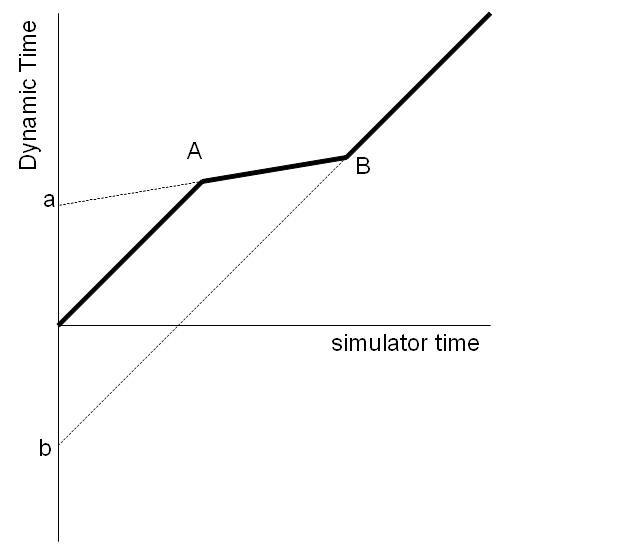
\includegraphics[width=3.2736in,height=2.85in]{figures/Timedyntime.jpg}
\caption{Illustration of how Dynamic Time can vary with Simulator Time, 
and the resulting effect on the offset between them.}
\end{center}
\end{figure}

\end{enumerate}}


\classitem{TimeEnum} Base-class

This class contains no methods, just an enumeration.

\begin{enumerate}
\item Julian.
\item Modified Julian.
\item Truncated Julian.
\item Calendar.
\item Clock.
\item Days since epoch.
\item Seconds since epoch.
\end{enumerate}



\classitem{TimeGMST}
  \textref{TimeStandard}{ref:TimeStandard}

{\begin{enumerate}
\funcitem{set\_time\_by\_trunc\_julian}
Even though GMST is technically a Standard Time, Truncated Julian Time
has no meaningful interpretation, since it is based on a synodic clock.
 This function overrides the one inherited from \textref{TimeStandard}{ref:TimeStandard}
by causing a termination if anything attempts to use Truncated Julian
Time in GMST.

\funcitem{calculate\_calendar\_values}
Even though GMST is technically a Standard Time, the calendar that is an
element of Standard Time  has no meaningful interpretation, since it is
based on a synodic clock.  This function overrides the one inherited
from \textref{TimeStandard}{ref:TimeStandard} by causing a termination if anything
attempts to use a calendar in GMST.

\end{enumerate}}



\classitem{TimeGPS}
 \textref{TimeStandard}{ref:TimeStandard}


GPS time is somewhat unusual.  It fits the definition of a Standard Time
(it is well defined), but does not maintain the same counters as a
typical clock.  Instead of days, months, etc., it uses weeks and
seconds of week since epoch (there is also a \textit{rollover} count,
used because the number of weeks since epoch has now exceeded its
counting capacity of 1,024 weeks).

{\begin{enumerate}
\funcitem{calculate\_calendar\_values}
The conventional concept of calendar makes no sense in the GPS
timekeeping system.  All GPS values are maintained all of the time, and
any call to this function will produce a code termination.

\funcitem{set\_time\_by\_days}
Converts number of days since epoch into weeks and seconds of week since
epoch.

\funcitem{set\_time\_by\_seconds}
Converts number of seconds since epoch into weeks and seconds of week
since epoch.

\funcitem{set\_time\_by\_trunc\_julian}
The epoch is hard-coded in Truncated Julian Time, so it is trivial to
convert any given Truncated Julian Time and change that into days or
seconds since epoch.

\end{enumerate}}
\classitem{TimeManager} Base-class


{\begin{enumerate}
\funcitem{get\_converter\_ptr}
As each converter is registered, it is stored in a vector and is assigned an
index value equal to its position within that vector.  
This function returns a pointer to any particular
converter given its index in that vector.

\funcitem{get\_time\_change\_flag}
The \textit{time-change-flag} is triggered if the Dynamic Time scale
factor is changed (see \textref{update\_offset}{ref:updateoffset}).  
This function simply returns
the boolean indicating whether the scale factor changed since the last
time step.

\funcitem{get\_time\_ptr}
There are two instances of this function, one takes a name, and the
other takes an index.  When a time representation is registered with
the Time Manager, a pointer to it is stored in a vector.  All time
representations also have a unique name.  This function returns the
pointer to the time representation using either value as a reference.

\funcitem{initialize}
Registers and initializes the Dynamic Time.

Counts the number of time-types registered from the S\_define.

Calls \textit{TimeManagerInit::initialize\_manager}.

Runs an update on all time-types at Dynamic Time = 0.0.

\funcitem{register\_converter}
Called from the S\_define level, this function simply appends a pointer to
each converter onto the \textit{time\_converters\_ptrs}
vector.  This function is used when the converter is between two
specific time representations (e.g. TAI and UTC).

\funcitem{register\_generic\_converter}
Called from the S\_define level, this function simply appends a pointer to
each converter onto the \textit{time\_converters\_ptrs}
vector.  This function is used when one or both of the two time
representations is not a Standard Time (i.e. is a UDE or MET).  This
function requires naming the non-Standard representation to identify
which representation is intended.

\funcitem{register\_time\_named}
This function is generally called from the S\_define for a non-Standard Time
representation, using the representation's name as an
identifier.  It adds each of these representations into the registry of
time-types.

\funcitem{register\_time}
This function is called from the S\_define for each Standard Time
representation (Standard Times are already named).  It adds each of these 
representations into the registry of time-types.

\funcitem{time\_standards\_exist}
Returns a boolean value, indicating whether there are any time
representations that fall into the \textit{TimeStandard} classification.

\funcitem{time\_lookup}
\label{ref:timetypeslookup}Each time-type has its own class, and is
registered with the Time Manager, with a pointer to the class in a
vector registry.  The location of the time-type in the registry is the
\textit{index} of that time-type.  The index is also stored in each
class, as is the name of the class.

The index of a time-type is the point of reference throughout the
simulation, and the address of the memory of a particular time-type can
easily be found from the Time Manager, if the index is known.  If only the name
is known, this method provides a technique for obtaining the index from the
name, thus allowing access to the memory address by name only.

With a name input, the function returns the index associated with that
name.  The default return value is -1, which is returned if no
time-type by that name can be found.

In the event that a time-type with no defined name is used (the name
{\textquotedblleft}undefined{\textquotedblright} is the default name for all
time-types), the
return value is -2.

For each registered time-type, the \textit{name }variable is compared
with the lookup name.  When a match is found, the index value is
changed from -1 to the \textit{index} variable of that time-type.  The
remainder of the time-types are still checked before returning.  If a
match is found and the index value is not equal to -1, there is a
problem:  the routine has found two occurrences of a time-type with the
same name.  It is not possible to distinguish between them, and the
code terminates.

\funcitem{update}
This function is the master function once the simulation has begun.  It
is called from the S\_define with the Simulator Time as its argument (i.e., 
\textit{sys.exec.out.time}, or its equivalent for non-Trick
simulations).

\begin{enumerate}
\item First, Simulator Time is updated, taking the value of the input argument.
\item Next, the update functions are called on all subclasses of Time.
\item The last step is necessary only in simulations in which time
reverses direction;  if time reverses at the current time, the offset
between sim-time and TimeDyn will change.
\end{enumerate}

Note that while steps \textit{i. and ii.} are only followed if the argument is
different from the previously recorded Simulator Time (\textit{sim\_time}), 
step
\textit{iii.} must be followed with every call.  This is deliberate, and is
essential due to the way time is updated during the dynamic integration
procedures.  These procedures can advance the \textit{sim\_time} value to the
next Simulator Time before the simulation engine can process any commands at
that Simulator Time; a command to reverse time will then be received after the
time has been advanced to the instant at which the change should take place,
causing a delay in its effect if step \textit{iii.} were not processed.

\funcitem{verify\_table\_lookup\_ends}
This method exists within all time representations, by inheritance from
\textref{Time}{ref:Time}.  The Time Manager method runs through all registered 
time
representations, calling the respective methods.
\end{enumerate}}


\classitem{ TimeManagerInit}  \label {ref:timemanagerinit} 
  Base-class


{\begin{enumerate}
\funcitem{create\_init\_tree}
\label{ref:createinittree}This function is used only during
initialization; it creates the tree structure by which time-types
are initialized to their starting values.

The user should specify a time-type to be used for initialization.  If
that is not done, or an invalid entry is made, then the following
sequence of steps occur:


\begin{enumerate}
\item When the method 
\textref{TimeManager::time\_lookup}{ref:timetypeslookup}
is
called to find the initializer\_index, none will be found and the
initializer\_index will return with value -1 (invalid entry) or -2 (not
defined).
\item An invalid entry will cause termination of the code in
\textref{verify\_times\_setup}{ref:verifytimessetup}.
\item An undefined entry will cause termination of the code in
\textref{verify\_times\_setup}{ref:verifytimessetup}
if there is more than one time
representation (i.e. anything in addition to Dynamic Time).
\end{enumerate}

\bigskip
In the event that no initialization was defined, and only Dynamic Time
is present, then Dynamic Time starts at 0.0, as it always does. No
initialization is necessary.  This method is processed trivially.

A {\textquotedblleft}status{\textquotedblright} method is used to keep
track of which time-types have been entered into the tree.  Initially,
all time-types are assigned a status value of 0.  The Dynamic Time is
then assigned value -2, and the initializer time the value 1, being the
first level on the initialization tree (potentially overriding the
Dynamic Time assignment).

Each time-type with status 0 is tested; if the user has carefully
defined the tree with an
{\textquotedblleft}initialize\_from{\textquotedblright} assignment for
this time-type, the method \textit{add\_type\_initialize}(on page
\pageref{ref:addtypeinitialize}) 
specific to
that time-type is called to add the time-type to the tree.  This
function is iterative, it tests the parent type, and the
parent's parent until it finds a type already in the
tree (status {\textgreater} 0).  If the chain terminates before a type
already in the tree is found, no action is taken.

If the user has not carefully defined the tree, this function will look
for the time-type with the lowest status {\textgreater}0 (i.e. highest
on the tree) for which a valid converter exists to initialize the
current time-type.

This search algorithm is processed as follows:

{\begin{enumerate}
\item As long as one or more time-types remain to place in the tree, and all
possibilities have not been exhausted, the following steps are taken.

{\begin{enumerate}
\item Set \textit{num\_added\_pass} to 0.
\item Increment \textit{seeking\_status}
\begin{itemize}
\item \textit{seeking\_status} identifies the `level' of the
tree being tested.  
\item On the first pass, (\textit{seeking\_status = 1}),
time-types are tested for entry into the tree structure 
directly under the \textit{initializer}.
\item On the second pass, (\textit{seeking\_status = 2}) the level beneath 
that is tested, etc.  
\item If, at some level, nothing can be added (\textit{num\_added\_pass  = 0} 
at the end of
the pass) then everything that can be added has been added; the algorithm is
complete, or it has failed.
\end{itemize}

\item For each time-type that is not yet in the tree:

\begin{itemize}
\item If it has a defined time-type from which to initialize, add it to
the tree (recursively adding its parent as necessary).
\item If it does not have a defined time-type from which to initialize,
test it using status \textit{seeking\_status} 
to determine whether an appropriate converter
function exists.  If it does, add the type to the tree with status
\textit{seeking\_status+1}.  If not, wait for the next pass.
\end{itemize}

\item The total number of types in the tree (\textit{num\_added\_total})
is incremented by
\textit{num\_added\_pass}, and the code loops back to step A.

\end{enumerate}}

\item If the code processes a path without further addition
(\textit{num\_added\_pass = 0}) and there is still something to add
($num\_added\_total < num\_types$), then the algorithm has failed and
the code terminates.
\end{enumerate}}

\funcitem{create\_update\_tree}
\label{ref:createupdatetree}This function provides much the same
functionality by the same method as that described in
\textref{create\_init\_tree}{ref:createinittree}, 
except that it considers the update tree. 
The only substantial difference comes in the recording of the tree; the
initialization tree is recorded within TimeManagerInit, while the
update tree is recorded in TimeManager.  Also, while the initialization
happens only once, the update happens repeatedly, so the update sequence
is introduced and recorded.  This necessitates an additional function,
\textref{set\_ordered\_update\_list}{ref:setorderedupdatelist}.

\funcitem{organize\_update\_list}
\label{ref:setorderedupdatelist} While the user may specify times in any 
order in the S\_define file, the Time Manager must have a record of the
order in which to update the different representations.  Since Dynamic
Time updates directly from Simulator Time, it must be updated first. 
Then TAI is typically updated from Dynamic Time, and then the other
derived times.  While the initializer (\textit{TimeManagerInit}) builds the 
tree
for the update procedure, the Time Manager uses this function to reorganize 
the \textit{time\_vector}, which it then uses to ensure that
representations are always updated before their respective dependents. 

\funcitem{get\_conv\_ptr\_index}
\label{ref:getconvptrindex}As each converter is registered, it is stored
in a vector, with some index value.  As each time representation is
registered, it is also stored in a different vector, again with some
index value.  Each converter operates between two time representations.
 A variable \textit{converter\_ptrs\_index }provides the lookup
capability to find a particular converter given two time
representations.




Consider the value  $x=Ni_{\text{from}}+i_{\text{to}}$\textit{ , }with 
\textit{N}
representing the number of time-types,  $i_{\text{from}}$ the index of
the representation from which the conversion is to be made, and 
$i_{\text{to}}$ the index of the time representation to which the
conversion is to be made.  Then the
\textit{x}\textit{\textsuperscript{th}}\textit{ }element in 
\textit{converter\_ptrs\_index }is set to be  an integer equal to the
location of the converter in the converter registry that will convert
from $i_{\text{from}}$ to  $i_{\text{to}}$.




This method receives the value \textit{x}, and returns the index in the
converter registry.  An invalid input, or an input for which there is
no registered converter causes the method to return a value -1.  




Note that since converters are bidirectional the same result is
obtained from  $x=Ni_{b}+i_{a}$ and from   $x=Ni_{a}+i_{b}$

\funcitem{get\_conv\_dir\_init}
\label{ref:getconvdirinit}In addition to tracking the index of the
converters, it is also necessary to track the versatility of those
converters, and in which direction they should be used.  For example,
the converter between TAI and UTC (\textit{TimeConverter\_TAI\_UTC})
can be used in either direction.  Sending the value appropriate to a
conversion from TAI to UTC into 
\textref{get\_conv\_ptr\_index}{ref:getconvptrindex}
 will return information on the index (and hence the memory location) 
 of this converter, but not how to use it.  There are two
additional tables that provide directional information on usage of the
converter, one for initialization
(\textit{init\_converter\_dir\_table}), and one for updates
(\textit{update\_converter\_dir\_table}).




While \textit{converter\_ptrs\_index }is symmetric,\textit{ }the
converter direction tables are not.  Passing in 
$x=Ni_{\mathit{TAI}}+i_{\mathit{UTC}}$(from TAI to UTC) will return a
value of +1, while passing in a value of  
$x=Ni_{\mathit{UTC}}+i_{\mathit{TAI}}$(from UTC to TAI) will return a
value of -1.  If a converter is not valid (e.g. Dynamic Time to TAI is
valid at run-time, but not at initialization, while TDB to TAI is valid
neither at runtime nor initialization), then the entry in the
appropriate table has value 0.




This method returns the value for the converter at initialization.

\funcitem{get\_conv\_dir\_upd}\label{ref:getconvdirupd}
See \textref{get\_conv\_dir\_init}{ref:getconvdirinit} for details.  This 
method returns the
value for the converter at run-time.

\funcitem{get\_status}
During the construction of the initialization and update trees
(\textref{create\_init\_tree}{ref:createinittree} and
\textref{create\_update\_tree}{ref:createupdatetree}), each time 
representation has a status
corresponding to its location in the tree.  This function returns the
status of any given time representation.

\funcitem{increment\_status}
During the construction of the initialization and update trees 
(\textref{create\_init\_tree}{ref:createinittree} and
\textref{create\_update\_tree}{ref:createupdatetree}), each time 
representation has a status
corresponding to its location in the tree.  This function sets the
status of a time-type to be one higher than that of its parent.

\funcitem{initialize}
Sets the references \textit{dyn\_time\_index }and
\textit{initializer\_index.}

Calls \textref{verify\_times\_setup}{ref:verifytimessetup} to ensure that the 
time-type
settings are mutually consistent.

Allocates memory for several arrays, and initializes some values.

\funcitem{initialize\_manager}
\label{ref:initializemanager}Comprises a series of calls, all to methods
within this class:


\begin{enumerate}
\item \textit{initialize}
\item \textit{populate\_converter\_registry}
\item \textit{verify\_converter\_setup}
\item \textit{create\_init\_tree}
\item \textit{initialize\_time\_types}
\item \textit{create\_update\_tree}
\end{enumerate}


\funcitem{initialize\_time\_types}
This method starts by initializing the head of the initialization tree
with the appropriate call to \textit{initialize\_initializer\_time. 
}Then, it progresses through the remaining time representations calling
their respective \textit{initialize\_from\_parent} methods on any time
types that have not been initialized.  This method is iterative, and
calls itself on the parent (in the initialization tree) if the parent
has not been initialized.  Eventually, it must find an initialized
representation (since the head of the tree has been initialized).

\funcitem{populate\_converter\_registry}
This method sets the values of the converter tables discussed in
\textref{get\_conv\_ptr\_index}{ref:getconvptrindex}, 
\textref{get\_conv\_dir\_init}{ref:getconvdirinit}, and
\textref{get\_conv\_dir\_upd}{ref:getconvdirupd}.

\funcitem{set\_status}
During the construction of the initialization and update trees
(\textref{create\_init\_tree}{ref:createinittree} and
\textref{create\_update\_tree}{ref:createupdatetree}), each time 
representation has a status
corresponding to its location in the tree.  This function sets the
status of a time-type to some input value.

\funcitem{verify\_times\_setup}
\label{ref:verifytimessetup}Makes a number of sanity checks that the
time-types are mutually compatible and that there are no
inconsistencies in the way the time module was set up.  In particular,
it ensures that the simulation can be initialized, and that there are
no duplicate time representations.

\funcitem{verify\_converter\_setup}
This method verifies that those converters that need special
considerations (at this time, this only applies to those that use data lookup
tables) are appropriately configured.



\end{enumerate}}
\classitem{TimeMessages}
This is the message handler for the \timeDesc. It contains no methods.


\classitem{TimeMET}
 \textref{TimeUDE}{ref:TimeUDE}

Mission Elapsed Times have the built-in capability to `hold' their progression
for some period.  Beyond the typical UDE data, this class contains an
additional boolean value, \textit{hold}.
% and \textit{previous\_hold}
\begin{enumerate}

\funcitem{update}
MET contains two values that indicate whether a hold is active, \textit{hold} 
and \textit{previous\_hold}.  The former is set externally, the latter is set 
within this method and provides a comparison data point to identify when 
\textit{hold} has been changed.

If MET has just transitioned to a hold, the regular update method is run to 
bring MET up-to-date with the time at which the hold was commanded, and 
\textit{previous\_hold} is transitioned to \textit{false}.

If MET is in a hold, and was previously in a hold, no action is taken.

If MET is not in a hold, and was not previously in a hold, the inherited 
update method is called. 

Finally, if MET has just transitioned from a hold, the time converter is 
updated to reset the offset between this type and its parent.  The actual 
value of MET does not require updating, because it retains its current value 
until the next time-step.

Note that when the hold flag is being toggled, it is beneficial to set the 
Time Manager's \textit{simtime} value to 0. The Time Manager compares that 
value to the Simulator Time to determine whether to call the individual 
update methods; setting it to zero forces the update method.  Without this 
step, this update method may be bypassed, and processed at the time-step after 
it was intended.
\end{enumerate}

\classitem{TimeStandard}
\label{ref:TimeStandard}
 \textref{JeodBaseTime}{ref:Time}


{\begin{enumerate}
\funcitem{add\_type\_initialize}
This function is intended to add a time-type to the initialization tree
if its parent is already in the tree, and to recurse on its parent if
the parent is not in the tree.  

Initially, two values are set:


\begin{enumerate}
\item The status of the time-type is changed from 0 to -1 for reasons
explained later.  
\item Then, the \textref{time\_types\_lookup}{ref:timetypeslookup} function is 
called to
obtain the index value of the parent type.  
\end{enumerate}



This function causes the code to terminate on any of the following three
conditions:


\begin{enumerate}
\item The parent type cannot be found.  This function is only called if
the user has named the parent type.  If the user has done so, but not
registered the type with the Time Manager, there is the potential for
serious malfunction.
\item The status of the parent is -1.  This can only be achieved when
the parent has already been processed by this function within the
current recursion chain, which indicates that the user has specified a
circular initialization path.
\item If no converter exists to convert the parent time into the child
time-type.  The user has specified that this converter should be used,
but failed to provide the converter.
\end{enumerate}

The next step is the recursion component:  if the parent is not in the
tree (status = 0), and has a defined parent itself, then carry out this
same function on the parent.

If the parent is in the tree (either by being in the tree originally, or
by a result of the previous command), then add the type and increment
\textit{num\_added\_pass}.  If not, set the status of the type back to
0 (indicating that the type has not been added to the tree), and return
to the calling function.

{\itshape
Note -- if this was called recursively, the return of status 0 will
cause the child's status to go to 0, all the way down
the chain until it returns to create\_init\_tree. }

\funcitem{calculate\_calendar\_values}
\label{ref:calculatecalendarvalues}Converts the time in any
representation from a Truncated Julian format into a Gregorian calendar
format.  The algorithm for this conversion is non-trivial.

The calendar format has both regular and irregular cyclical variations: 
there are always 60 seconds in a minute, 60 minutes in an hour, and 12
months in a year.  There are 24 hours in a day, except for the addition
of leap seconds, although these can be factored in relatively easily. 
There are 28-31 days per month, with known predictability.  There are
365-366 days in a year, with leap years occurring in a known pattern: there is 
a leap year every 4 years, excepting one every 100 years, excepting one every 
400
years (there are 24-25 leap years every 100 years, and always 97 leap
years in a 400-year period).  There are 146,097 days in any 400-year
period.

The most difficult challenge in converting from Julian to Gregorian is
in identifying the month number.  This can be achieved through integer
division (which is faster than a lookup) if care is taken to avoid the
irregularities associated with the leap-day February 29, and the uneven
nature of the days-per-month distribution.  

{\itshape
[A basic application of integer division fails almost immediately: with
31 days in January, the divisor must be {\textgreater} 31 and
{\textless} 32 to produce the same answer for days 1-31 but not for day
32.  Then, the same answer is produced for days 32-62, but day 62 is
either March 2 or March 3, not February as intended.]}

The first of these irregularities can be accounted for if the starting
time is chosen carefully.  To avoid an
{\textquotedblleft}if-else{\textquotedblright} clause on the leap-day,
it makes sense to make the leap-day the last day of the year.  Then, if
the year requires 366 days, it is added automatically, and if the year
has only 365 days, there is no February 29 because the date rolls to
the next year first.  Consequently, the epoch is placed on March 1. 
Furthermore, it should be on March 1 immediately after a leap-day so
that some residual partial day can build until a leap-day is needed
after 4 years.  The 100-year and 400-year cycles complicate this, and
by the same argument, the epoch should be on March 1 after a 400-year
leap-day.  It is chosen then that the epoch date be March 1, 1600.

The epoch date for Truncated Julian Time (May 24, 1968) happens to occur
134,493 days after the March 1, 1600, epoch.  

After obtaining the year information from the Julian Date, the second
irregularity (uneven nature of days-per-month) is accounted for by
adjusting the epoch time slightly.  This is explained in step 10 (``x.'') 
below.

The algorithm for converting Truncated Julian Time into Gregorian
calendar then is described by:

\begin{enumerate}
\item Take the integer part of the Truncated Julian Time  
$TJT_{int}=int(TJT)$, where \textit{TJT } represents Truncated Julian Time, and
$TJT_{int}$ the integer part thereof.
\item The fraction of the current day that has elapsed is first
represented as a number of minutes. 
${min}=1440\left({TJT}-{TJT}_{int}\right)$
\item The fractional part of the last minute provides the seconds value
of the clock. 
${seconds}=60\left({min}-int(min)\right)$
\item An additional term, \textit{clock\_resolution }is used to force
\textit{seconds } to `tick-over' to 0
if the value is sufficiently close to 60.  This keeps the data-stream
more uniform.  If the clock is forced to
`tick-over', that requires that the
minutes value be incremented by 1, and a check made as to whether that
action also caused the day to
`tick-over'. 

(\textit{e.g. July 7 23:59:59.999999999999 = July 8 0:0:0.0})
\item The hour of day is found from an integer division, by 60, of the
integer representation of minutes-of-day.  Then the clock minutes value
is equal to the remainder.

\begin{equation*}
{hour}=\frac{{min}_{\text{int}}}{60},
\end{equation*}
\begin{equation*}
{minute}={min}_{\text{int}}-60\cdot {hour}.
\end{equation*}
 

\item If the value \textit{julian\_day }(the integer part of TJT + any
increment from step iv) has not changed from its previous value, the
algorithm is completed.  If it has, the more cumbersome task of
determining the date is undertaken.
\item Calculate \textit{julian\_day }by adding 134,493 to adjust for
epoch, 

${julian}\text{\_}{day}={TJT}_{\text{int}}+134493$.

(134,493 represents the number of days from the conversion epoch to the 
Truncated
Julian epoch).  

March 1, 1600, is day 0, not day 1; this is not an
arbitrary decision, but necessitated by the mathematical structure.
\item Calculate \textit{n\_400,} the number of 400-year periods since
March 1, 1600, by dividing the number of days by 146,097 (days per
400-year period).  Since March 1, 1600, is day 0, then March 1, 2000, is
day 146,097, and falls into the next 400-year period.
\item  Calculate \textit{r\_400, }the number of days since the end of the last
400-year period (i.e., since March 1, 1600, or March 1, 2000).  In the next
step, it becomes necessary to treat March 1 as day 1 rather than day 0;
hence we also add 1:


\begin{equation*}
r_{400}={day}-146097n_{400}+1 \; \; , \; \; r_{400}\in [1,146097]
\end{equation*}


\item Calculate \textit{n\_100, }the number of 100-year periods in the
current 400-year period.  The first three 100-year periods have 36,524 days,
the fourth has 36,525 days.  

In the case that March 1 was represented by day
0, the last day in the fourth period would be day
146,096.  A suitable divisor would have to be $x>36524$ to make 
$(146096/x)<4$.  But then day 36,524 would fall into the first period,
when it should be the first day in the second period.  

In the case that
March 1 is counted as day 1, then the last day in the
fourth period is 146,097.  Once again,  $x>36524$, but
now day 36,524 correctly falls into the first period, as the last day.  
$x=36524.3$ is an appropriate number such that the last days in each
period are 36,524; 73,048; 109,572; and 146,097.  Because this divisor is
non-integer, integer arithmetic cannot be utilized; instead, cast the
result to an integer, in effect taking the integer part of the result.

\begin{equation*}
n_{100} = int ( r_{400} / 36524.3 )
\end{equation*}

\item Calculate \textit{r\_100}, the number of days since the last
100-year period (March 1, 1900, or March 1, 2000).  There are 36,524
days in each of the first three 100-year periods in any 400-year period, so
subtract the appropriate multiple of 36,524.  In the next step, the last
period is no larger than earlier periods, and integer arithmetic can be
utilized if March 1 is counted as day 0.  Hence, the extra day is
removed again.  

\begin{equation*}
r_{100}=r_{400}-36524n_{100}-1\; \; , \; \; 
r_{100}\in[0,36524].  
\end{equation*}

\item Calculate \textit{n\_4}, the number of 4-year periods.  There are
1,461 days in the first 24 of these, and 1,460 days in the
25\textsuperscript{th}, unless  $n_{100}=3$ in which case the
25\textsuperscript{th} period also has 1,461 days.  


\begin{equation*}
n_{4}=r_{100}/1461 \; \; , \; \; n_{4}\in [0,24]
\end{equation*}
 
\item Calculate  

\begin{equation*}
r_{4}=r_{100}-1461n_{4}+1 \; \; , \; \;  r_{4}\in [1,1461].  
\end{equation*}

The
next step has the last period being larger than the earlier periods
again, so again add 1 to make March 1 be represented as day 1.
\item Calculate the number of whole years in the
current 4-year period.  Again, this real result is cast to an integer.
\begin{equation*}
n_{1}=r_{4}/365.3 
\end{equation*}

\item Calculate  
\begin{equation*}
r_{4}'=r_{4}+2n_{1}+30,
\end{equation*}
a value to be used in
evaluating the month number.  Because the month length fluctuates, the
epoch is adjusted such that March 1, 2000, is day 31.  Two additional
days are added each year, so that February 28, 2001, is day 395, and
March 1, 2001, is day 398.  This unusual strategy effectively gives
February 30 days, smoothing out the month-to-month fluctuations.  It
also puts the epoch on February 1, 1600.
\item Calculate  

\begin{equation*}
m'=\text{int}\left(\frac{r'}{30.585}\right)
\end{equation*}

With approximately 30.585 days per month, the number of months in the 4-year
period can be determined.


\item Calculate  
the month
number.  
\begin{equation*}
m=m'+2-12\left(\frac{m'+1}{12}\right) 
\end{equation*}
This first adjusts \textit{m'} accounting for
February \textit{(m=2) }being counted \textit{as m' =
0, 12, 24, 36, 48.  }The second adjustment accounts for the whole
years; the integer division in the parentheses
{\textquotedblleft}rolls{\textquotedblright} each January
\textit{(m' = 11, 23,35,47), }reducing the value of
\textit{m} from its December value.
\item Calculate \textit{d}, the day number on the current month.  With
30.585 days per month,  

\begin{equation*}
d=r'-\text{int}\left(30.585m'\right)
\end{equation*}

with the
second term being an integer equal to the cumulative number of days at
month's end (February -- 30, March -- 61, April -- 91,
May -- 122, etc.)

\item Calculate \textit{y}, the year.  

\begin{equation*}
y=1600+400n_{400}+100n_{100}+4n_{4}+\left(\frac{m+1}{12}\right)
\end{equation*}

\end{enumerate}
The calendar could now be expressed as  yyyy/mm/dd::hr:min:sec.sec




This is usually only necessary when outputting values in a required
format; the simulation runs on Truncated Julian Time only, with no
reference to the calendar time.  Consequently, this function is not
called as part of the regular time update.




\funcitem{calendar\_update}
Each Standard Time has several potential ways of being presented,
including purely decimal values (seconds since epoch, days since epoch,
Truncated Julian Time), and a calendar.  The decimal representations
are more computationally efficient, and are maintained in current
status throughout the simulation.  Maintenance of the calendar
representation is more time-consuming, and is only called as needed on
a type-by-type basis.  This function checks whether the simulation has
advanced since the last calendar update.  If it has,
\textref{calculate\_calendar\_values}{ref:calculatecalendarvalues} 
is called to convert the
decimal representation into a calendar representation.

\funcitem{ convert\_from\_calendar}
\label{ref:convertfromcalendar}This function is intended for use during
initialization, when data values are read in as a calendar format (more
commonly used), and must be converted to a a decimal format for
propagation within the simulation.




Six values are input -- year, month, day, hour, minute, and second.

The algorithm basically follows the inverse process of that presented in
\textref{calculate\_calendar\_values}{ref:calculatecalendarvalues}.


\begin{enumerate}
\item The number of years since epoch is 
\begin{equation*}
y={year}-1601+\left(\frac{{month}+9}{12}\right)
\end{equation*}

(notice that this integer division term
{\textquotedblleft}rolls{\textquotedblright} each March)
\item The value, \textit{y}, can then be divided into a number of
400-year periods, plus a number of 100-year periods, etc.  

\begin{align*}
n_{400} &=\frac{y}{400} \\
n_{100} &=\frac{y-400n_{400}}{100} \\
n_{4} &=\frac{y-400n_{400}-100n_{100}}{4} \\
n_{1} &=y-400n_{400}-100n_{100}-4n_{4}  \\
m &={month}-2+12\left(1-\frac{{month}+9}{12}+n_{1}\right)
\end{align*}

$m$ is the month number in the 4-year period starting March 1.


\item The Truncated Julian Time can now be calculated:

\begin{enumerate}
\item The fractional part of the day is\ \ 
\begin{equation*}
{TJT}_{1}=\frac{{second}}{86400.0}+\frac{{minute}}{1440.0}+\frac{{hour}}{24.0}
\end{equation*}

\item Each day counts as {\textquotedblleft}1{\textquotedblright}
\begin{equation*}
{TJT}_{2}={TJT}_{1}+{day}
\end{equation*}

\item The month value,\textit{ m}, is complicated.  In 
\textref{calculate\_calendar\_values}{ref:calculatecalendarvalues} 
the method was developed by which the
epoch was adjusted by 30 days (actually, by 31, because  1 day had
already been added to make March 1 day 1 instead of day 0), and 2 days
added each year to smooth out the month-to-month variations.  With
these modifications, it was possible to carry out integer arithmetic,
using 30.585 days per month and taking the integer part of the result.
That same method can be used here: the number of days is calculated
from\textit{ m, }then the 2 days per year and the 31 day-offset
removed.  
\begin{equation*}
{TJT}_{3}={TJT}_{2}+\left({int}\left({30.585 m}\right)-2n_{1}-31\right)
\end{equation*}

\item By setting the epoch to March 1, 1600, the number of days in each
completed 4-year, 100-year, and 400-year period is known and fixed. 
The final step is to remove the 134493 day offset between March 1, 1600,
and May 24, 1968, the epoch of Truncated Julian Time. 




\begin{equation*}
{TJT}={TJT}_{3}+1461n_{4}+36524n_{100}+146097n_{400}-134493
\end{equation*}
Note -- $n_1$ is not included because
\textit{m} counts the number of months in a 4-year period.
\end{enumerate}
\item Finally, days since epoch is simply the difference between current
Truncated Julian Time, and the stored value of Truncated Julian Time at
the epoch.  Seconds since epoch is then trivially calculated.
\end{enumerate}



\funcitem{initialize\_from\_parent}
Takes the value of the time in the representation that is parent to this
one in the initialization tree, and converts it to this time.  This is
a recursive function, and will call itself on the parent type if the
parent has not yet been initialized.

\funcitem{initialize\_initializer\_time }
Typically, the simulation starts at some prescribed time in some
prescribed time representation.  This function takes the input data and
uses it to initialize the prescribed time representation (in the event
that it is a Time Standard).  There are several formats in which that
initial time can be presented:


\begin{enumerate}
\item {\bfseries
calendar}

Calls \textref{convert\_from\_calendar}{ref:convertfromcalendar} to generate 
the decimal
representation.
\item {\bfseries
Julian}

Converts directly to Truncated Julian, and from there to days and
seconds.
\item {\bfseries
Modified Julian}

Converts directly to Truncated Julian, and from there to days and
seconds.
\item {\bfseries
Truncated Julian}

Converts to days and seconds.
\item {\bfseries
Seconds since epoch}

Converts to days and Truncated Julian Time.
\item {\bfseries
Days since epoch}

Converts to seconds and Truncated Julian Time.
\end{enumerate}



If the user does not specify the format, the code will attempt to
interpret what was intended, but any ambiguity will result in
termination.

\funcitem{julian\_date\_at\_epoch}
Simply returns the epoch as a Julian, rather than Truncated Julian
value.

\funcitem{seconds\_of\_year}
This method relies on the calendar functionality included with \JEODid.  Two 
variables are included in the Time Standard class, 
\textit{seconds\_at\_year\_start}, and \textit{year\_of\_last\_soy}.  The 
former records the value of the variable \textit{seconds} at the beginning of 
the current year; the latter records to which year
\textit{seconds\_at\_year\_start} pertains.

First, the calendar is brought up-to-date (if it is not already so).  Then the 
code divides into 3 paths:

\begin{enumerate}
	\item When \textit{calendar\_year = year\_of\_last\_soy} (most 
	frequent path).  This path simply differences the current value of 
	\textit{seconds} from the value at the start of the year.
	\item When \textit{calendar\_year = year\_of\_last\_soy + 1} AND
  $calendar\_month \leqslant 2$ (unusual).  This path requires that the year 
  has ticked over once since the last time this method was accessed, and the 
  current month is January or February.  The value \textit{seconds\_of\_year} 
  is calculated directly, and used to define a new value for 
  \textit{seconds\_at\_year\_start}; \textit{year\_of\_last\_soy} is also 
  redefined.
	\item All other cases.  This path is most often accessed during the 
	first call to this method for any of the time-types.  Otherwise, it 
	would be a rare circumstance that would lead to this path.  It 
	temporarily reassigns the current time to be the start of the year, 
	calculates the \textit{seconds} value there, then returns to current 
	time.  The calculated value becomes \textit{seconds\_at\_year\_start}, 
	the current year becomes \textit{year\_of\_last\_soy}, and the 
	calculation of \textit{seconds\_of\_year} is then trivial.
\end{enumerate}




\funcitem{set\_time\_by\_seconds}
Uses the version in \textref{JeodBaseTime}{ref:Time}, and adds conversion to 
Truncated Julian Time.

\funcitem{set\_time\_by\_days}
Uses the version in \textref{JeodBaseTime}{ref:Time}, and adds conversion to 
Truncated Julian Time.

\funcitem{set\_time\_by\_trunc\_julian}
Given a Truncated Julian Time, converts it into days since epoch and
seconds since epoch.





\end{enumerate}}

\classitem{TimeTAI}
  \textref{TimeStandard}{ref:TimeStandard}.


Inherits completely from \textit{TimeStandard}.


\classitem{TimeTDB}
  \textref{TimeStandard}{ref:TimeStandard}

Inherits completely from \textit{TimeStandard}.

\classitem{TimeTT}
  \textref{TimeStandard}{ref:TimeStandard}

Inherits completely from \textit{TimeStandard}.

\classitem{ TimeUDE}
\label{ref:TimeUDE}
 \textref{JeodBaseTime}{ref:Time}.


{\begin{enumerate}
\funcitem{add\_type\_initialize}
Works in much the same way as the \textref{TimeStandard}{ref:TimeStandard}
version of the
method of the same name, but adds additional protection to verify that
the representation that defines the epoch (as well as the parent) of
this representation is configured correctly and already established in
the initialization tree, and that the representation from which this
will be updated at run-time is defined and available.

\funcitem{clock\_update}
Given the decimal representation of time elapsed since epoch, this
method generates a clock (day::hour:minute:second) representation. 




\funcitem{convert\_epoch\_to\_update}
\label{ref:convertepochtoupdate}In the case where a UDE has an epoch
defined in one representation, and ticks with (i.e. is updated from)
another (e.g. a clock may start at some known UTC time, but tick with
TAI), this method temporarily converts the specified epoch time into
the {\textquotedblleft}ticks-with{\textquotedblright} representation,
in order to calculate the offset between this representation and the
{\textquotedblleft}ticks-with{\textquotedblright} representation.




That offset is then used by the converter to provide the standard
conversion at run-time.




The only complicating issue in this routine occurs when the converter
between the epoch-definition type and the
{\textquotedblleft}ticks-with{\textquotedblright} type has already been
initialized.  Under some circumstances, the initialization of a
converter establishes the converter for a restricted period of time,
and the epoch could lie outside that range.  To be safe, the converter
is de-initialized, and re-initialized at the epoch value, then
de-initialized again (if it is needed later, at run-time, it will be
re-initialized with values appropriate for the simulation time).




\funcitem{initialize\_from\_parent}
This function is used in the situation in which a simulation is
initialized with respect to some other known time-type, and this time-type
representation fits somewhere -- other than at the head -- in the
initialization tree.




The \textit{parent} in this case is the representation from which this
one will be updated at run-time.  If that has not been initialized,
this function (or its parallel in \textref{TimeStandard}{ref:TimeStandard}, as
appropriate) is called for the \textit{parent.}




There are two methods by which a UDE can be initialized when it is not
at the head of the initialization tree -- either by specification of
its value at simulation-start, or by specification of an epoch.




In order to initialize a UDE by specifying the epoch, it is necessary to
temporarily step out of the current time, and go to the epoch time of
the UDE.  First, the current value of the \textit{parent} is stored
off, then the algorithm branches in a multi-path solution.





\begin{enumerate}
\item The simplest case is one in which the \textit{parent} is also the
representation in which the epoch is defined; in that case the
\textit{parent} value at simulation-start is overwritten with the
\textit{parent }value at the epoch\textit{.}


\item In the situation that the two differ, the following procedure is used:

\begin{enumerate}
\item A converter is found between the epoch-defining type and the
\textit{parent }type, and initialized if necessary.  If no converter
exists, the code must terminate.  Note: this step is only carried out
here in the case that the epoch-defining type is itself a UDE;
otherwise, this step is more complicated and is carried out in
\textref{convert\_epoch\_to\_update}{ref:convertepochtoupdate}, 
but it must be carried out at some
point.
\item If the epoch-defining type has already been initialized, its value
must also be stored off temporarily and overwritten with the value at
epoch.
\item  The epoch-defining type is then populated with the epoch
definition, and converted to the \textit{parent }type using
\textref{convert\_epoch\_to\_update}{ref:convertepochtoupdate}.  
At this time, the \textit{parent}
defines the epoch just as well as the epoch-defining type does; the
epoch-defining type can now be reverted to its former configuration,
and we can proceed as though the epoch-defining type and the parent
type were the same.
\end{enumerate}
\end{enumerate}



The final step requires the initialization of the converter between the
UDE and the \textit{parent.  }For this, we can use the current values
of both:


\begin{enumerate}
\item The UDE has value 0.0 if the initialization is based on an epoch
definition, and some other defined value if the initialization is based on an
initial value.
\item The \textit{parent} has value equal to that at the
UDE's epoch if the initialization is based on an epoch
definition, and the appropriate value at simulation start if the
initialization is based on some initial value.
\end{enumerate}
Either way, the offset between the two types can now be calculated, and
used throughout the rest of the simulation.




If the \textit{parent }configuration has been altered during the course
of this routine, it must now be reverted to its original configuration,
and that value used to initialize the UDE for the time corresponding to
the start of the simulation.

\funcitem{initialize\_initializer\_time }
This method is used to initialize the UDE time in the case that the UDE
time is being used to initialize the simulation (i.e., it is at the head
of the initialization tree).  To properly initialize the UDE in this
situation, it must have an epoch defined in some other representation,
and an initial value at simulation-start.  

One additional requirement
on this type of initialization is that the epoch cannot be defined as
being in some other UDE, and if there are any
Standard Times in the simulation the epoch must be a Standard Time (the epoch 
can be defined in Dynamic
Time, but only if there are no Standard Times included).

Verification is made that the two variables
\textit{TimeManagerInit::sim\_start\_format } and
\textit{TimeUDE::initial\_value\_format} are consistent, and the
initial values are then set as defined.

Verification is then performed on the epoch definition, ensuring that
the epoch-defining type and epoch values are defined appropriately, and
that there is no conflicting definition in the value of the epoch.

Next, the initializing value of the UDE is converted into the
\textit{parent} representation (the clock from which the UDE will be
updated at run-time). To initialize the converter for this purpose, it
is usually necessary to first consider the epoch values, since data
must be known at both ends of the converter before it can be
initialized.  For this representation, the initial values are stored,
then it is set to zero.  The epoch-defining representation is set to
its predefined value.  If the \textit{parent} and epoch-defining
representation are different, the epoch-defining values are converted
to \textit{parent }values, thus providing the value for parent and this
representation at the same instant in time.  Once the converter is
initialized, the initial values for this representation  are restored,
and used to set the simulation-start values in \textit{parent}.

\funcitem{must\_be\_singleton}
Returns \textit{false}, there may be multiple instances of UDE times.

\funcitem{set\_epoch\_dyn}
Makes several checks that the epoch format and epoch values are
consistent with an epoch defined in Dynamic Time, then sets the value
of Dynamic Time to that specified as the epoch.

\funcitem{set\_epoch\_std}
Makes several checks that the epoch format and epoch values are
consistent with an epoch defined in  a Standard Time, then sets the
value of that time to that specified as the epoch.

\funcitem{set\_epoch\_times}
Calls one of


\begin{itemize}
\item set\_epoch\_dyn
\item set\_epoch\_std
\item set\_epoch\_ude
\end{itemize}
depending on whether the epoch is defined in Dynamic Time, in a Standard
Time, or in another UDE time.




\funcitem{set\_epoch\_ude}
Makes several checks that the epoch format and epoch values are
consistent with an epoch defined in  a UDE Time, then sets the value of
that time to that specified as the epoch.

\funcitem{set\_initial\_times}
Verifies that the initial value of this representation is not
over-constrained (e.g. by setting both seconds-since-epoch and
clock-seconds), then propagates the specified value to other formats
(e.g. converts a clock format to days-since-epoch and
seconds-since-epoch).

\funcitem{set\_time\_by\_clock}
Converts a clock input format into days-since-epoch and
seconds-since-epoch.




\funcitem{set\_time\_by\_days}
Converts a days-since-epoch input format into and seconds-since-epoch
and a clock.

\funcitem{set\_time\_by\_seconds}
Converts a seconds-since-epoch input format into and days-since-epoch
and a clock.

\funcitem{verify\_epoch}
Verifies that the epoch representation, the values specified for the
epoch, and the format in which they are specified are appropriate.

\funcitem{verify\_init}
Verifies that the initial values specified for this representation, and
the format in which they are specified are appropriate, then calls
\textit{set\_initial\_times} to assign those values.

\funcitem{verify\_update}
Verifies that the \textit{parent} representation is defined
appropriately.

\end{enumerate}}



\classitem{TimeUT1}
  \textref{TimeStandard}{ref:TimeStandard}.


Inherits almost completely from \textit{TimeStandard}, with only one
additional method:

{\begin{enumerate}
\funcitem{get\_days}
Simply returns the value \textit{days} (days-since-epoch).
\end{enumerate}}


\classitem{TimeUTC}
  \textref{TimeStandard}{ref:TimeStandard}.

Inherits completely from \textit{TimeStandard}


\end{enumerate}}




\clearpage

\subsection{Default data files}
This section describes the data files included with the release
of \JEODid.

{\begin{enumerate}
\funcitem{tai\_to\_ut1.cc}
This file gives a tabulation of the differences between \textit{TAI} and
\textit{UT1} as a function of \textit{TAI}.

Instructions for updating this file are contained in the Extension
section of the User Guide (chapter \ref{ch:user}).

\funcitem{tai\_to\_utc.cc}
This file gives a tabulation of the differences between \textit{TAI} and
\textit{UTC} as a function of \textit{UTC}.

Instructions for updating this file are contained in the Extension
section of the User Guide (chapter \ref{ch:user}).

\end{enumerate}}



\clearpage
\subsection{Extensibility}
The Time Representations Model is designed in such a way that it can
easily be extended with the addition of more time representations.

Each new time representation must meet the following requirements:


\begin{enumerate}
\item It shall be included as a class of its own, inheriting from JeodBaseTime
or TimeStandard.
\item It shall have a name
\item It shall have a constructor and destructor
\item There shall be some method for deriving its value from one of the
time classes that already exist.
\end{enumerate}



A new time representation must have a new Time Converter.  A user may
also wish to define a new Time Converter to convert directly between two
preexisting time representations (e.g., UT1 to MET).

Each new Time Converter must meet the following requirements:

\begin{enumerate}
	\item A converter shall be defined to allow the derivation of the new
	time representations.
	\item The converter shall be included in a class of its own, inheriting
	from \textit{TimeConverter}.
	\item The converter class shall define one or both of the methods
\begin{enumerate}
	\item \textit{convert\_a\_to\_b}.
  \item \textit{convert\_b\_to\_a}.
\end{enumerate}
  \item The converter class shall define the \textit{valid\_directions} attribute to specify when \textit{convert\_a\_to\_b} and/or \textit{convert\_b\_to\_a} is valid.
  \item The converter class shall have an \textit{initialize} method.
  \item The converter class shall have a constructor and a destructor.
\end{enumerate}

Instructions for adding these methods are found in the Extension section
\vref{sec:User_Extension} of the User Guide.

%\section{Version Inventory}
%%%%%%%%%%%%%%%%%%%%%%%%%%%%%%%%%%%%%%%%%%%%%%%%%%%%%%%%%%%%%%%%%%%%%%%%%%%%%%%%%
%
% Purpose:  Inventory of files for the time model
%
% 
%
%%%%%%%%%%%%%%%%%%%%%%%%%%%%%%%%%%%%%%%%%%%%%%%%%%%%%%%%%%%%%%%%%%%%%%%%%%%%%%%%


\section{Inventory}
All \timeDesc\ files are located in the directory \newline
{\tt \$\{JEOD\_HOME\}/models/environment/time}.
Relative to this directory,
\begin{itemize}
\vspace{-0.2\baselineskip}
\item Header and source files are located
in the model {\tt include} and {\tt src} subdirectories.
Table~\ref{tab:source_files} lists the
configuration-managed files in these directories.
\vspace{-0.1\baselineskip}
\item Data files are located in the model {\tt data} subdirectory.
See table~\ref{tab:data_files}
for a listing of the
configuration-managed files in this directory.
\vspace{-0.1\baselineskip}
\item Documentation files are located in the model {\tt docs} subdirectory.
See table~\ref{tab:documentation_files}
for a listing of the
configuration-managed files in this directory.
\vspace{-0.1\baselineskip}
\item Verification files are located in the model {\tt verif} subdirectory.
See table~\ref{tab:verification_files}
for a listing of the
configuration-managed files in this directory.
\end{itemize}

\input{inventory}


\chapter{User Guide}\hyperdef{part}{user}{}\label{ch:user}
%----------------------------------
The User Guide is divided into 3 components, one for each of three
different types of user.

The Analysis section of the user guide is intended primarily for
users of preexisting simulations.
It comprises the following elements:
\begin{itemize}
\item A description of how to modify \timeDesc\ variables after
the simulation
has compiled, including an in-depth discussion of the input file;
\item An overview of how to interpret (but not edit) the S\_define
file;
\item A sample of some of the typical variables that may be logged.
\end{itemize}

The Integration section is intended for simulation
developers.
It describes the necessary configuration of the \timeDesc\
within an
S\_define file, and the creation of standard run directories.  The
latter
component assumes a thorough understanding of the preceding Analysis
section of the user guide.
Where applicable, the user may be directed to selected portions of
Product Specification (Chapter \ref{ch:spec}), or to examples in the tutorial or
Verification and Validation chapter (Chapter \ref{ch:ivv}).

The Extension section is intended primarily for
developers
needing to extend the capability of the \timeDesc.  Such users
should have a
thorough understanding of how the model is used in the preceding
Integration section, and of the model
specification (described in Chapter \ref{ch:spec}).


\section{Analysis}
%%%%%%%%%%%%%%%%%%%%%%%%%%%%%%%%%%%%%%%%%%%%%%%%%%%%%%%%%%%%%%%%%%%%%%%%%%%%%%%%%
%
% Purpose:  Analysis part of User's Guide for the ModelName model
%
% 
%
%%%%%%%%%%%%%%%%%%%%%%%%%%%%%%%%%%%%%%%%%%%%%%%%%%%%%%%%%%%%%%%%%%%%%%%%%%%%%%%%

% \section{Analysis}
\label{sec:User_Analysis}
\subsection{Overview of the Time Representations}
Typically, a simulation will contain a \textit{time} object, which will
contain a time manager, and possibly some additional number of time
representations.  There are three fundamentally distinct time concepts
working in JEOD:


\begin{itemize}
\item Simulator Time
\item Dynamic Time
\item Derived Time
\end{itemize}



Simulator Time provides the behind-the-scenes simulator control.  For
Trick users, this is the value \textit{sys.exec.out.time.} It provides
the information necessary to ensure that functions are called in the
appropriate order, that tasks are queued appropriately, and to query
whether a task has already been completed.  In general, it must be
incremental, i.e. always advancing forwards.  Simulator Time is not a
part of the \timeDesc, since it does not measure a physical passage of
time.

Dynamic Time is the time used for representing the physics.  When
physical constants rely on a timescale (e.g. speed of light, meters
\textit{per second}), it is the Dynamic Time to which they refer.
Consequently, this is the time used by the integrators.  The Dynamic
Time is automatically included with the Time Manager.

Derived Time has unbounded possibilities, with the ability to represent
any clock that the user chooses, as long as that clock is somehow
related to Dynamic Time.  To find which times are available, open the
S\_define file, find the \textit{time }object, and look for statements
similar to these following:

\begin{verbatim}
 environment/time:  TimeTAI   tai;
 environment/time:  TimeUTC   utc;
 environment/time:  TimeUT1   ut1;
\end{verbatim}

There will be one of these statements for each additional Derived Time.
Within the concept of Derived Time, there are two sub-concepts:


\begin{itemize}
\item Standard Time
\item User-Defined Time
\end{itemize}
These are described in more detail below.

\subsubsection{Dynamic Time (\textit{manager.dyn\_time}, class \textit{TimeDyn})}
The Dynamic Time must be present in any simulation, but will not
appear by itself in the S\_define file.  It always has initial value 0.0, and
counts the number of SI seconds (\textit{manager.dyn\_time.seconds) }elapsed
since the simulation began.  Note that this may not be the same as the
Simulator Time (e.g. \textit{sys.exec.out.time}), since
Dynamic Time has the capacity to run at different rates -- even
in reverse -- whereas the simulator clock is simply an incremental
counter.  The simulation dynamics are all based on Dynamic Time.

\subsubsection[Standard Times (class TimeSTD)]{Standard Times (TimeSTD)}
The concept of a Standard Time is that it is commonly accepted, with no
ambiguity.  Picking a particular value on a particular clock (e.g. noon
on January 23, 2009, UTC) is well understood without additional
context.  Consequently, there can be only one clock running in a
simulation for each of these times (any more would be redundant).
JEOD 2.0 is released with
the following commonly used Standard Times, although this list may have been
extended by your simulation developer.


\begin{itemize}
\item TAI (International Atomic Time) is the most closely linked to
Dynamic Time.  It ticks at the same rate, but starts with a simulation-specific
initial value, defined by the user.  Most derived times are derived
from TAI; this is found in almost all simulations.
\item UTC (Coordinated Universal Time) is the standard clock on Earth.
If initializing the simulation at a particular time, this is usually
handled with UTC.  It ticks at the same rate as TAI, but occasionally
has leap seconds introduced to keep it near-synchronous with UT1.  The
historical record of the occurrence of leap seconds is provided.  If a
simulation happens to span a time at which a leap second was
introduced, UTC will be updated accordingly.  The user may override the
value corresponding to the offset between TAI and UTC, as described in the \reftext{data override section}{ref:data_override}.
\end{itemize}

\begin{itemize}
\item UT1 (Universal Time) is based on the solar day (whereas UTC is
based on days of 86,400 SI seconds).  It ticks at an irregular
rate, a result of a variable rotation rate of Earth, caused by
tidal friction, polar motion, and tectonic action, among others.  The
difference between UTC and UT1 is therefore variable, and not highly
predictable, although it is always less than 1 second (when the
differences become too large, a leap second is added to UTC to bring
them close again -- see figure \ref{fig:TAIUTCUT1}.  For historical simulations, calibrated data is
provided to convert directly from TAI to UT1.  For simulations outside
the range of the provided data, the offset will be held at the last
known value; no attempt is made to predict offsets.  Instructions for
overriding this value are provided in the \reftext{data override section}{ref:data_override}.  Instructions for updating
the calibrated data set with the most recently available data are provided in the \reftext{data update section}{ref:data_update}.


\begin{quotation}
Special Notes Re: previous versions of JEOD:
\begin{enumerate}
\item In this version, the offsets between TAI and UTC, and between
TAI and UT1, are updated continuously, whereas the time management in JEOD 1.x.y identified the offset
at the start of the simulation only, and used that offset throughout
the simulation.  For backward compatibility, the new updates can be
turned off by setting the flags true\_utc and true\_ut1 to
false. This should only
be done for tests that require backward compatibility for comparison to
simulations conducted in JEOD 1.x.
\item In JEOD 1.x.y, the data for generating UT1 was simply the DUT1 value - the difference between UTC and UT1.  In JEOD 2.0, UTC is no longer the ``fundamental'' second, and the preferred conversion method to get UT1 is to do so from TAI.  Therefore, simply using DUT1 to override the tai\_to\_ut1 conversion value will produce error.  The conversion must be from TAI to UT1, therefore attempting to override the data requires additional consideration of the number of leap seconds (UTC to TAI conversion) in order to generate the TAI to UT1 conversion.  Alternatively, a converter could easily be written to generate UT1 from UTC directly, but this has been deliberately omitted from the general release to avoid confusion over identifying the preferred method for generating UT1.  Overriding the data is not recommended for general practice.
\end{enumerate}
\end{quotation}



\begin{figure}[htp]
\begin{center}
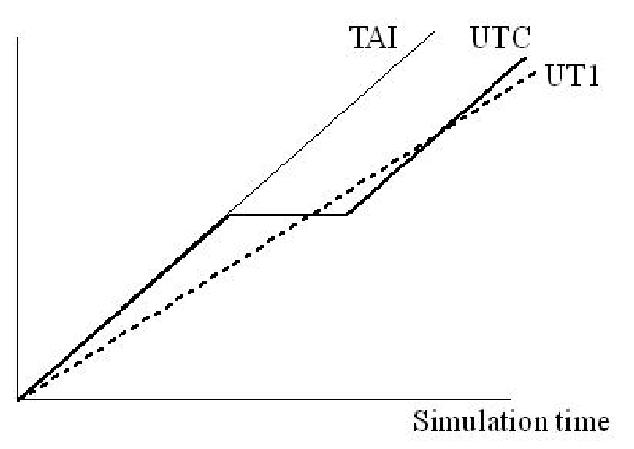
\includegraphics[width=3.2736in,height=2.85in]{figures/Timetaiutcut1.jpg}
\caption{Illustration of the relative evolution of TAI, UTC, and UT1
values, and how leap seconds are used.}
\label{fig:TAIUTCUT1}
\end{center}
\end{figure}


\item GMST (Greenwich Mean Sidereal Time) is based on a sidereal clock
(1 sidereal day = 1 rotation period, approximately 23 hours and 56 minutes
on a synodic clock).  There are 24 sidereal hours in a sidereal day, 60
sidereal minutes in a sidereal hour, and 60 sidereal seconds in a
sidereal minute, although these are rarely -- if ever -- used.
\item GPS (Global Positioning System time) ticks at the same rate as TAI
and is simply offset by a known value, but counts in weeks and seconds
of week rather than days, or the conventional calendar found in TAI.
\item TT (Terrestrial Time) ticks at the same rate as TAI, and is simply
offset by a known value.  It is used in ephemeris models.
\item TDB (Barycentric Dynamic Time) ticks at an obscure rate that
accounts for the relativistic corrections introduced by
Earth's orbital eccentricity.  Since TAI is geocentric
(the clocks are located at the bottom of Earth's
gravitational well, and move with Earth), it is not the best clock for
solar-system missions; TDB removes the geo-effects from TAI.
\end{itemize}



\subsubsection[User-Defined Times (TimeUDE)]{User-Defined Times (TimeUDE)}
The main distinction between a Standard Time and a User-Defined Time is
that User-Defined Times are ambiguous without additional context.  A
commonly used example of a UDE (User Defined Epoch) is Mission Elapsed
Time.  Simply stating that a simulation started two hours after the
mission started is not a very meaningful statement, unless we also have
information on when the mission started.  The \textit{epoch} of UDEs
(i.e. when their value was zero) must be defined before they make any
sense at all; that epoch must ultimately be anchored with a Standard
Time, or with the Dynamic Time.  A secondary difference arises from the
ambiguity of a UDE time; while Standard Times are restricted to one
instance per time-type, the UDEs have no such restriction.  A dozen or
more different clocks could be running simultaneously, representing
different time zones (ticking with UTC), or different mission-elapsed
times for simulations involving multiple vehicles.

There are two types of UDE:


\begin{itemize}
\item UDE:  These have an epoch defined in one time type, and tick in
lockstep with another (may be different).
\item MET (Mission Elapsed Time):  This special type of UDE also has the
ability to halt periodically, to allow for occurrences such as
pre-launch hold points.  The basic UDE will keep ticking through such
hold points.
\end{itemize}



\subsection{Available Data}
This section describes the output data that a user is most likely to
need, identified by the major classes of data.

\subsubsection{JeodBaseTime}
JeodBaseTime is the base class of all time representations.  It contains the
following variables (among others):

\begin{itemize}
\item {\textit{name}} simply names the time object
\item {\textit{days}} represents the current time as some decimal number of elapsed days since epoch
\item {\textit{seconds}} represents the current time as some decimal number of elapsed seconds since epoch
\item {\textit{initial\_value}} is the value of \textit{seconds} at the start of the simulation.
\end{itemize}

\subsubsection[Dynamic Time (time\_dyn)]{Dynamic Time (time\_dyn)}
Dynamic time inherits those data from JeodBaseTime and simply counts SI seconds,
and days, elapsed since the start of the simulation.  It also contains
a variable, \textit{scale\_factor}, that allows it to deviate from the
simulator time (\textit{e.g. sys.exec.out.time}), although changing
this value is not recommended for a beginning user.

\subsubsection[Standard Times]{Standard Times}
The Standard Times also inherit from Time, and add the following
variables:


\begin{itemize}
\item {\itshape
calendar\_year}
\item {\itshape
calendar\_month}
\item {\itshape
calendar\_day}
\item {\itshape
calendar\_hour}
\item {\itshape
calendar\_minute}
\item {\itshape
calendar\_second}
\item {\itshape
trunc\_julian\_time}
\item {\itshape
julian\_date}
\item {\itshape
tjt\_at\_epoch}
\end{itemize}



Truncated Julian Time (\textit{trunc\_julian\_time}) is used as the basic anchor
for each clock, giving each one a basis for measuring ``absolute'' time, and
setting the offsets between the clocks.  It
represents the number of days elapsed since
midnight on May 23 / 24, 1968, as measured in its own clock.
That means that Truncated
Julian Time = 0 in Terrestrial Time (TT) does NOT represent the same
instant as Truncated Julian Time = 0 in Universal Coordinated Time
(UTC).

Julian Date is the original basis for Truncated Julian Time, but has its epoch
much farther in the past, so has fewer available signigificant digits for
precision work.  Like
Truncated Julian Time, it has a distinct value in each clock at any specific
instant in time, and is related to Truncated Julian by:
\begin{equation*}
Julian = Truncated-Julian + 2440000.5
\end{equation*}
in all clocks.
Because of its loss of precision, Julian Date should be used for reference
purposes only.


In most Standard Times (excepting GPS and GMST), \textit{seconds} and
\textit{days} are the primary operational data.  They represent elapsed
time since some fixed epoch (default is J2000, or 12:00 noon TT on January 1,
2000). This is the same instant in time across the different clocks;
the difference between the \textit{trunc\_julian\_time} representation
and the \textit{seconds} representation is best seen in this example:
\begin{quotation}
Terrestrial Time (TT) ticks in lockstep with atomic time (TAI), but they
are offset by a constant value.  The J2000 epoch occurred at the same
instant for both, so \textit{seconds} (since J2000) will be the same
for both since they tick in lockstep.  Conversely, the Truncated Julian
Time {\textquotedblleft}epochs{\textquotedblright} are clock-dependent,
so they occurred at different instants.  Since TT and TAI are offset
from each other, their \textit{trunc\_julian\_time} values will always
differ by a constant amount.
\end{quotation}

The epoch can be easily configured to any desired time, J2000 was chosen simply
because it is a well known data point.
Setting the epoch closer to the simulation
time would give a smaller value on the elapsed time, allowing for more precise
time interval specifications (using J2000 as the epoch does allow microsecond
significance, which is adequate for most purposes).  Note that changing the
epoch WILL NOT affect the precision of absolute time, since that will still be
based on Truncated Julian Time (currently with significance of $O(10^{-5}) s$).
In contrast, the \textit{julian\_date} variable has only millisecond
significance.

To anchor the operational values of \textit{seconds }and \textit{days}
to a fixed time, the value \textit{tjt\_at\_epoch} provides the
Truncated Julian Time at the instant that \textit{seconds = 0.0.}

While seconds and days are trivially incremented throughout the
simulation, the calendar variables require a more time-consuming
update, and so are updated only as necessary.  The simulation developer
may (or may not) have scheduled these, and some time representations
may have calendars that are updated regularly, some rarely, some never.
 To check how often those updates are scheduled, look at the S\_define
file for the statements similar to:


\begin{verbatim}
      {DYNAMICS, environment) environment/time: time.utc.calendar_update(
              In  double  simtime =  sys.exec.out.time);
\end{verbatim}

Note that the simtime argument is used for the purposes of verifying
that the update is actually needed (occasionally, calendar updates are
called behind the scenes by other routines, so if time has not advanced
since it was last updated, it will not be updated again).  The actual
time data is pulled directly from the time object, in this case,
\textit{utc.  }




\subsubsection{User-Defined-Epoch Times (TimeUDE)}
Again, these inherit from Time, but add the following variables:


\begin{itemize}
\item {\itshape
epoch\_year}
\item {\itshape
epoch\_month}
\item {\itshape
epoch\_day}
\item {\itshape
epoch\_hour}
\item {\itshape
epoch\_minute}
\item {\itshape
epoch\_second}
\item {\itshape
clock\_day}
\item {\itshape
clock\_hour}
\item {\itshape
clock\_minute}
\item {\itshape
clock\_second}
\item {\itshape
epoch\_format}
\item {\itshape
initial\_value\_format}
\item {\itshape
epoch\_defined\_in\_name}
\end{itemize}
The \textit{epoch\_***} values are the values of the clock (declared by
name in \textit{epoch\_defined\_in\_name}) at which the UDE time starts
(i.e. has value = 0.0).

The \textit{clock\_*** }values function comparably to the
\textit{calendar\_*** }variables found in the Standard Times; they
provide the dd::hh::mm::ss clock value of the current time, measured in
time elapsed since epoch.  They may also be used to set the epoch of one
UDE by specifying it in terms of the \textit{clock\_***} value of another
UDE.

Note that UDE times do not include year and
month, since these are not well-defined quantities outside of a
standard time reference (a day is 86,400 seconds, while a month is some
variable number of days).

\subsection{Initializing the Simulation}
In any application where specific absolute times are needed (e.g.,
ephemeris), the simulation must be initialized to some known value.  The
start of the simulation always has a Dynamic Time value of 0.0, but may
have a UTC value of 2005/Jan/23::15:30:05 (as an example).
Initialization in this context means setting the starting times
correctly.  This section describes how to do that.




In very basic simulations, there may be no need for an absolute
reference time, nor a second clock.  In that case no additional times
should be declared in the S\_define, and only \textit{dyn-time} used.  Since
\textit{dyn-time} will always start running at 0.0, that eliminates the need for
an initialization process.  The code will terminate if the user
includes any additional clocks (beyond the default Dynamic Time) but
fails to specify a method for initializing the simulation.

Where initialization is required, those values are set in an input file
or modified-data file, discussed below.

\subsubsection{Initialization requirements}
The following is a list of requirements pertinent to initialization.
This is provided as a reference so that the user can identify the
capability of the \timeDesc.


\begin{itemize}
\item The initialization is available from any Standard or UDE time.
\item The initialization time can be expressed in any of the following
formats:

\begin{itemize}
\item Gregorian calendar (Standard Times only)
\item dd::hh::mm::ss clock format (UDE Times only)
\item Julian, Modified Julian, or Truncated Julian formats (Standard Times only)
\item days since epoch
\item seconds since epoch
\end{itemize}
\item Initializing a UDE Time (such as Mission-Elapsed-Time) requires
that the UDE be anchored to another defined time representation.  The
following options are available:

\begin{itemize}
\item Given an absolute UDE epoch time (defined with respect to some
other Derived Time (e.g. 0.0 UDE (tjt)= 123.456 TAI (tjt))) and an
absolute start time from some Derived Time of known epoch (e.g.
sim\_start = 123.456 UTC (tjt)), then the initial value of the UDE time
can be calculated.
\item Given an absolute UDE epoch time and UDE initial value, then the
absolute start time can be calculated and used to initialize other
times, and the simulation.
\item Given an absolute simulation-start time from some Derived Time and
an initial value for the UDE time, then the absolute UDE epoch time
(mission start time) can be determined.
\end{itemize}
\end{itemize}






\subsection{Input Files}
\subsubsection{Defining the initialization time with a Standard Time}
If some real time is to be used to start the simulation, it must be
expressed in some representation (e.g. UTC).  The first value to
specify is that representation, and it must be specified by name.

\begin{verbatim}
time.time_manager_init.initializer ="UTC";
\end{verbatim}




Next, the format in which the time is expressed must be declared.  This
could be Julian, modified\_julian, truncated\_julian, or calendar.
Obviously, the choice is determined by the data available to the user.
The choice must be preceded by
{\textquotedblleft}TimeEnum::{\textquotedblright} as in the example
below.


\begin{verbatim}
time.time_manager_init.sim_start_format = TimeEnum::calendar;
\end{verbatim}

In this case, calendar was chosen, it is now necessary to fully define
the mission start time in a calendar format on a UTC clock.

\begin{verbatim}
time.utc.calendar_year = 1998;
time.utc.calendar_month = 12;
time.utc.calendar_day = 31;
time.utc.calendar_hour = 23;
time.utc.calendar_minute = 59;
time.utc.calendar_second = 50.0;
\end{verbatim}

If the start time were known in a Truncated Julian format on the UT1
clock, for example, this may have looked like:

\begin{verbatim}
time.manager_init.initializer = "UT1";
time.manager_init.sim_start_format = TimeEnum::truncated_julian;
time.ut1.trunc_julian_time = 12345.6789;
\end{verbatim}

The code has some internal verification processes that will catch most
of the common errors that users are likely to make in defining these values,
but it is always
better to get it right the first time.



\subsubsection {Initializing a UDE or MET / Setting the Epoch for a UDE or
MET}

There are two values that all clocks take at simulation-initialization:
\begin{itemize}
\item A definition of its epoch (the time at which it had a value of 0.0)
\item Its value at the start of the simulation.
\end{itemize}

Standard clocks have a default epoch already defined.  Dynamic Time has an
automatic epoch of ``now''.  User-Defined-Epoch clocks (UDE and the more
flexible MET clocks) need additional definition.

Unless the UDE is being used to initialize the simulation, it is necessary
that only one of these is defined.  The other will be calculated.
Specifying both will overconstrain the system and lead to a failure.  If
the UDE is being used to initialize the simualtion, then both must be
specified.

There are multiple ways to directly specify the epoch of a UDE, including:
\begin{itemize}
\item as a calendar date and time in some standard clock,
\item as a Julian, Modified Julian, or Truncated Julian value in some standard
clock,
\item as some number of days or seconds elapsed since, or preceding, the epoch
of another clock (Standard or another UDE)
\item as some number of days or seconds elapsed since, or preceding, the start
of the simulation
\item as some time elapsed since, or preceding, the epoch of another UDE,
expressed in a clock format -- days, hours, minutes and seconds.
\end{itemize}

The sequence for setting the epoch is as follows:
\begin{enumerate}
 \item Decide on the clock to be used to define the epoch.
 \begin{itemize}
  \item Set the variable \textit{epoch\_defined\_in\_name} to the name of the
  chosen clock.  For example,
  \begin{verbatim}
        jeod_time.ude_clock.epoch_defined_in_name = "UTC"
  \end{verbatim}
  \item If setting it relative to simulation-start, use Dynamic Time
  (``Dyn'').
 \end{itemize}

 \item Decide on which option to use to numerically define the epoch.
 \begin{itemize}
  \item Set the value \textit{epoch\_format} accordingly to one of
  \begin{itemize}
   \item \textit{Julian} or \textit{julian}
   \item \textit{modified\_julian}
   \item \textit{truncated\_julian}
   \item \textit{calendar}
   \item \textit{clock}
   \item \textit{days\_since\_epoch}
   \item \textit{seconds\_since\_epoch}
  \end{itemize}
  \item  Note that not all options are available for all clocks.
  \begin{itemize}
   \item If setting relative to Dyn, use only \textit{days\_since\_epoch}
   or \textit{seconds\_since\_epoch}.
   \item If setting relative to another UDE, use only \textit{clock},
   \textit{days\_since\_epoch},
   or \textit{seconds\_since\_epoch}.
   \item If setting relative to a standard clock, use any option other than
   \textit{clock}.
  \end{itemize}
  \item Prepend your selection with \textit{trick.TimeEnum.}.  For example,
  to specify the epoch in a UTC calendar:
  \begin{verbatim}
        jeod_time.ude_clock.epoch_format = trick.TimeEnum.calendar
  \end{verbatim}

 \end{itemize}

 \item Set the numerical value(s) appropriate to your choice.
 \begin{itemize}
  \item If using \textit{calendar}, assign values to \textit{epoch\_year,
  epoch\_month, epoch\_day, epoch\_hour, epoch\_minute,} and
  \textit{epoch\_second}.
  \item If using \textit{clock}, assign values to \textit{clock\_day,
  clock\_hour, clock\_minute,} and \textit{clock\_second}.
  \item If using any of the other options, assign a value to
  \textit{epoch\_initializing\_value}.  This value is a dimensionless
  variable adopting units appropriate to its usage (i.e. days for the
  Julian and days-since-epoch options, and seconds for the
  seconds-since-epoch option).
  \item The \textit{epoch\_***} and \textit{clock\_***} variables can be set
  directly.  For example:
  \begin{verbatim}
       jeod_time.ude_clock.epoch_year = 1998
       jeod_time.ude_clock.epoch_month = 12
       jeod_time.ude_clock.epoch_day = 31
       jeod_time.ude_clock.epoch_hour = 23
       jeod_time.ude_clock.epoch_minute = 59
       jeod_time.ude_clock.epoch_second = 55.0
  \end{verbatim}
  \item The \textit{epoch\_initializing\_value} must be set with a call
  using the format:
  \begin{verbatim}
       jeod_time.ude_clock.set_epoch_initializing_value(0.0,<value>)
  \end{verbatim}
  The first argument must be 0.0, the second argument is the assigned
  value.
 \end{itemize}
\end{enumerate}

Alternatively, the epoch may be inferred by initializing the simulation
with respect to one clock, and setting the corresponding initial value of
the UDE.
The variable \textit{initial\_value\_format} specifies which data
set to look for  in  setting the initial value.  The options are:
  \begin{itemize}
   \item \textit{clock}
   \item \textit{days\_since\_epoch}
   \item \textit{seconds\_since\_epoch}
  \end{itemize}

If using \textit{clock}, assign values to \textit{clock\_day, clock\_hour,
clock\_minute,} and \textit{clock\_second}.  If using either of the other
options, assign a value to \textit{initializing\_value}.
Like \textit{epoch\_initializing\_value}, this value is a dimensionless
variable adopting units appropriate to its usage (i.e. days for the
days-since-epoch option, and seconds for the
seconds-since-epoch option).
The \textit{clock\_***} and \textit{initializing\_value} variables
may be set directly.  For example:
\begin{verbatim}
   jeod_time.ude_clock.initial_value_format = trick.TimeEnum.seconds_since_epoch
   jeod_time.ude_clock.initializing_value = -5.0
\end{verbatim}

This will start the clock with a value of -5.0 seconds, thereby placing its
epoch
5.0 seconds into the simulation.  Equivalently, the epoch could have been
set to be 5.0 seconds after the simulation start-time.  The two examples
presented here -- for setting the epoch and for setting the initial time --
are equivalent when used with the example in the previous section on
initializing the simulation from the UTC calendar representation.

Note that defining initial values for both \textit{initializing\_value} and
any of the \textit{clock\_***} variables will set up an internal conflict
and the code will fail.



\subsubsection{Initializing the simulation with a UDE or MET time}
To initialize the simulation with a UDE or MET time, that time must have
an epoch defined in some other time-type, and have an initial value with
respect to that epoch.  This is best seen in an example, such as at
\textit{verif/SIM\_5\_all\_inclusive/SET\_test/RUN\_UDE\_initialized/input.py}:

\begin{verbatim}
time.manager_init.initializer = "met_veh1"

time.metveh1.epoch_defined_in_name = "UTC"
time.metveh1.epoch_format = TimeEnum::calendar
time.metveh1.epoch_year = 1998
time.metveh1.epoch_month = 12
time.metveh1.epoch_day = 31
time.metveh1.epoch_hour = 23
time.metveh1.epoch_minute = 59
time.metveh1.epoch_second = 0.0

#///////////////////////////////////////////////////////////////////////
#// These two blocks are equivalent
#///////////////////////////////////////////////////////////////////////
time.metveh1.clock_day = 0
time.metveh1.clock_hour = 0
time.metveh1.clock_minute = 0
time.metveh1.clock_second = 50.0
#///////////////////////////////////////////////////////////////////////
#//time.metveh1.initial_value_format = TimeEnum::seconds_since_epoch
#//time.metveh1.initializing_value = 50.0
#///////////////////////////////////////////////////////////////////////

...

time.metveh1.update_from_name = "TAI";
\end{verbatim}
This example will start the \textit{metveh1} clock at a time corresponding to
1998/12/31::23:59:0.0 UTC.
The simulation will start when \textit{metveh1} = 50.0 seconds and
\textit{metveh1} will tick with TAI.
Note -- holds on MET
times can only be processed following simulation start, so in this example,
\textit{metveh1}
must have a value of 50.0 seconds at a time corresponding to 50.0 TAI-seconds
after the epoch time.

Since TAI and UTC are in lock-step during this interval, this example
is equivalent to
initializing the simulation at 1998/12/31::23:59:50.0 UTC, and setting the
initial value of \textit{metveh1} to 50.0 seconds.



\subsubsection{Defining the Trees}
The final part of the input file for time comprises setting up the
initialization and update trees.  Subject to the availability of
converter functions, any time type can (in principle) be initialized or
updated by any other time type.  However, it is recommended that TAI be
derived from Dynamic Time, and other types from TAI; in particular, due to
the implementation of leap seconds, TAI is not uniquely identified from all
UTC values, and TAI should never be updated from UTC.

\begin{verbatim}
time.time_tai.initialize_from_name ="UTC"
time.time_tai.update_from_name = "Dyn"
\end{verbatim}

This states that the initial value of TAI is going to be set by
the initial value of UTC (so there had better be a
UTC to TAI converter available and declared in the S\_define).  Folowing commencement of the simulation, TAI will continue to get its
values based on the value of Dynamic Time (\textit{manager.dyn\_time}). If
the user omits any part of the tree specification, the code has
sufficient capability that it can search for the most direct path to
provide a means of initializing or updating a time type that has no
specified path.  If such a path is found, a low-priority message will
be sent to the message handler to alert the user to the paths selected.
 The code will terminate immediately if any of the following conditions
are met:


\begin{itemize}
\item The user did not specify a full tree, and the auto-generator could
not find a suitable path.
\item The user sets up these paths in such a way that they generate
circular dependency (e.g. type XXX updates from YYY, and YYY from XXX).
\item A path is specified but there is no converter to handle the
conversion.
\item The specified initialization path does not form a continuous
connection from the initializer to each of the time types.
\item The specified update path does not form a continuous connection
from Dynamic Time to each of the time types.
\item The \textit{initializer} has a defined value for its
\textit{initialize\_from\_name} variable
(the \textit{initializer} gets its
initial data from user-input, not from another clock)
\footnote{If editing an existing simulation to use a different clock as the
\textit{initializer}, overwrite the new \textit{initializer}'s
\textit{initialize\_from\_name} so that it is empty (``''), and define a
value for \textit{initialize\_from\_name} for the old \textit{initializer}.}.
\end{itemize}

\subsubsection{Commanding changes mid-simulation}
The \textit{manager.update} routine checks the current Simulator Time with its recording of the Simulator Time the last time the Time Manager was called.
The user may specify changes to various values (e.g., start and stop a MET, change the scale-factor on the Dynamic Time) based on particular events, or on a predetermined Simulator Time-based schedule.  While those changes are implemented before the call is made to the \textit{manager.update} routine for a given Simulator Time, this is insufficient to ensure that the \textit{manager.update} routine is run with those changes set.

The problem lies in the behind-the-scenes interaction between the dynamic integrator and the Time Manager.  With some integrators (e.g. Runge-Kutta 4), the time must be evaluated at the end of the previous step as a component of the previous integration.  So at step \textit{i}, the value for time is needed at \textit{i, i+0.5,} and \textit{i+1}.  Once step \textit{i} is complete, changes made for step \textit{i+1} are implemented, and step \textit{i+1} begins; however, time has already been calculated at \textit{i+1}, and the update will not be called again for this instant of time without further intervention.

Therefore, it is recommended that whenever changes are being commanded, that the Time Manager's recorded value of Simulator Time be manipulated to ensure that when the \textit{manager.update} routine is called, the current Simulator Time will not agree with the recorded value.  A safe value is 0, since Simulator Time starts at 0 and always increments.

\begin{verbatim}
 read = 10
 time.metveh2.hold = true
 time.manager.simtime = 0
\end{verbatim}

\subsubsection{Turning off Warnings}
When setting the time, it is easy to overlook a critical step and finish with an
unrealistic time.  Fortunately, the most obvious errors are easily caught at
initialization by testing the value of Truncated Julian Time.  If it has a value
of
zero or less, a warning will be sent to the Message Handler.  Developers of
those historical simulations for which Truncated Julian Time should be less than
zero (i.e. pre-May 24, 1968) have an option to disable this warning message by
setting the flag \textit{send\_warning\_pre\_1968 = false}.


%\section{Integration}
%%%%%%%%%%%%%%%%%%%%%%%%%%%%%%%%%%%%%%%%%%%%%%%%%%%%%%%%%%%%%%%%%%%%%%%%%%%%%%%%%
%
% Purpose:  Integration part of User's Guide for the time model
%
% 
%
%%%%%%%%%%%%%%%%%%%%%%%%%%%%%%%%%%%%%%%%%%%%%%%%%%%%%%%%%%%%%%%%%%%%%%%%%%%%%%%%

 \section{Integration}\label{sec:Integration}

This section is intended for users who are incorporating the \timeDesc\ into a simulation.  It contains the basic requirements and step-by-step example of the construction of the \textit{Trick S\_define} file.  For more thorough examples, the verif directory in the standard release of \JEODid\ has a ``tutorial'' feel to it, stepping through from simple cases to more complex examples as it progresses from \textit{SIM\_1\_dyn\_only} through \textit{SIM\_5\_all\_inclusive}.


\subsection{S\_define requirements}
The time object in the S\_define is structured with the following
elements:


\begin{itemize}
\item Declare the following instances:

\begin{itemize}
\item TimeManager
\item TimeManagerInit
\item Desired time types (NOTE:  DynTime is automatically declared
within the TimeManager; declaring an instance of DynTime could cause a
failure when the code is confused about which version of DynTime to
use).
\item Desired time converters.  Note that converters may be
bidirectional, and that the code is sufficiently capable of
determining the appropriate direction.  This is important for the user
because the labels may be confusing; for example, the UTC to TAI
converter is labeled TAI\_UTC.  In the case that the converter is
desired in one direction at initialization, and the other during
simulation, IT IS NOT necessary to declare it twice.
\end{itemize}
\item Call the following initialization-class functions:

\begin{itemize}
\item The registration function for each of the declared time types to
register them with the Time Manager.  This function adds the time type
to the Manager's list, stores its location in that
list as a value in the time type itself, and stores the address of the
manager in each time type.
\item The registration functions for the declared time converters to
register them with the Time Manager.  This function adds the converter
to the Manager's list of available converters.
\item The Time Manager initialize function (NOTE -- this is a small
function that calls the main initialization functions in
TimeManagerInit).
\end{itemize}
\item Call the following run-time functions:

\begin{itemize}
\item The update function is called at any desired rate.  This will update
the decimal counter-type representation, \textbf{\textit{but not the
calendar representation}}, of all declared time-types.
\item \textit{(Optional) }the calendar-update function on any desired
time-types at any desired rate.  This function will convert the decimal
counter-type representation to a date::hr:min:sec representation.  Each
call to calendar\_update is type-specific and will update one,
\textbf{\textit{and only one,}} time-type.  Any call to the calendar-update will run the full decimal update method for all time-types if it has not already been done at that particular Simulator Time.  Consequently, the call to the regular update method is redundant if a calendar update is sequenced at the same rate.
\end{itemize}
\end{itemize}



\subsection{S\_define example}
\begin{enumerate}
\item First, declare the \textit{TimeManager} and \textit{TimeManagerInit} classes.  These
must be declared for all simulations.

\begin{verbatim}
 class TimeSimObject : public Trick::SimObject
 {
    jeod::TimeManager     manager;
    jeod::TimeManagerInit manager_init;

    ...

 };
\end{verbatim}



\item Next, in this example, I declare two additional time types, and two time converters
(there must be a converter from \textit{dyn}, and at least one per
declared time class.  In this case, the conversion path may be\textit{
dyn }to \textit{tai} to \textit{utc, }it will not be possible to go
from \textit{dyn }to \textit{utc }directly with these converters).

\begin{verbatim}
 class TimeSimObject : public Trick::SimObject
 {
    jeod::TimeManager     manager;
    jeod::TimeManagerInit manager_init;

    TimeTAI tai;
    TimeUTC utc;
    TimeConverter_Dyn_TAI  converter_dyn_tai;
    TimeConverter_TAI_UTC  converter_tai_utc;

    ...

 };
\end{verbatim}



\item Now I must register each of those types and their respective converters.
 The order in which this is done is not relevant; I chose to register
the time type, then immediately register the converter I plan to use for that time type; that order is just to keep track and ensure that I did not overlook
something.

\begin{verbatim}
 class TimeSimObject : public Trick::SimObject
 {
    jeod::TimeManager     manager;
    jeod::TimeManagerInit manager_init;

    TimeTAI tai;
    TimeUTC utc;
    TimeConverter_Dyn_TAI  converter_dyn_tai;
    TimeConverter_TAI_UTC  converter_tai_utc;

    TimeSimObject()
    {
        // Initialization jobs
        P_TIME ("initialization") manager.register_time( tai );
        P_TIME ("initialization") manager.register_converter( converter_dyn_tai );
        P_TIME ("initialization") manager.register_time( utc );
        P_TIME ("initialization") manager.register_converter( converter_tai_utc );

        ...

    }
 };
\end{verbatim}

\item Now initialize the manager.  This must be done for all configurations.

\begin{verbatim}
 class TimeSimObject : public Trick::SimObject
 {
    jeod::TimeManager     manager;
    jeod::TimeManagerInit manager_init;

    TimeTAI tai;
    TimeUTC utc;
    TimeConverter_Dyn_TAI  converter_dyn_tai;
    TimeConverter_TAI_UTC  converter_tai_utc;

    TimeSimObject()
    {
        // Initialization jobs
        P_TIME ("initialization") manager.register_time( tai );
        P_TIME ("initialization") manager.register_converter( converter_dyn_tai );
        P_TIME ("initialization") manager.register_time( utc );
        P_TIME ("initialization") manager.register_converter( converter_tai_utc );

        P_TIME ("initialization") manager.initialize( &manager_init );

        ...

    }
 };
\end{verbatim}

\item Next, schedule the regular updates.  This, also,  is required.  It will
update \textit{dyn}, \textit{tai} and \textit{utc}.

\begin{verbatim}
 class TimeSimObject : public Trick::SimObject
 {
    jeod::TimeManager     manager;
    jeod::TimeManagerInit manager_init;

    TimeTAI tai;
    TimeUTC utc;
    TimeConverter_Dyn_TAI  converter_dyn_tai;
    TimeConverter_TAI_UTC  converter_tai_utc;

    TimeSimObject()
    {
        // Initialization jobs
        P_TIME ("initialization") manager.register_time( tai );
        P_TIME ("initialization") manager.register_converter( converter_dyn_tai );
        P_TIME ("initialization") manager.register_time( utc );
        P_TIME ("initialization") manager.register_converter( converter_tai_utc );

        P_TIME ("initialization") manager.initialize( &manager_init );

        // Scheduled Jobs
        (DYNAMICS, "environment") manager.update( exec_get_sim_time() );
        ...
    }
 };
\end{verbatim}

\item Finally, I decided that the output from \textit{UTC} would be more
useful for my particular purpose if it were expressed as a calendar
format rather than a decimal format.  Here, I run the calendar update
at the same rate as the regular update, so that the calendar format is
always up-to-date with the decimal format.  Otherwise, the two values
may represent different times.

\begin{verbatim}
 class TimeSimObject : public Trick::SimObject
 {
    jeod::TimeManager     manager;
    jeod::TimeManagerInit manager_init;

    TimeTAI tai;
    TimeUTC utc;
    TimeConverter_Dyn_TAI  converter_dyn_tai;
    TimeConverter_TAI_UTC  converter_tai_utc;

    TimeSimObject()
    {
        // Initialization jobs
        P_TIME ("initialization") manager.register_time( tai );
        P_TIME ("initialization") manager.register_converter( converter_dyn_tai );
        P_TIME ("initialization") manager.register_time( utc );
        P_TIME ("initialization") manager.register_converter( converter_tai_utc );

        P_TIME ("initialization") manager.initialize( &manager_init );

        // Scheduled Jobs
        (DYNAMICS, "environment") manager.update( exec_get_sim_time() );
        (DYNAMICS, "environment") utc.calendar_update( exec_get_sim_time() );
    }
 };
\end{verbatim}

\end{enumerate}



\subsection{Updating the Data Tables}\label{ref:data_update}

Default data is provided for the offset between UTC and UT1, on a day-by-day basis,
from 1962 to the time just prior to to current JEOD version release date.  Data for the offset between TAI and UTC (the number of leap seconds) is also provided.  Because the UTC-UT1 offset changes continuously, this can quickly become outdated; the TAI-UTC data can also become outdated, but this is only updated once every 6 months so is not such a problem.
If the data available needs to be brought up-to-date, new data can be obtained from the International Earth Rotation and Reference Systems Service (IERS) webiste \href{http://www.iers.org}{http://www.iers.org}, which has links to Data/Products and Earth Orientation Data.

 If the user chooses to obtain their own data, we suggest the following steps:
 \begin{enumerate}

 \item Download the latest EOP 14 C04 (IAU2000) data file from the IERS at:

 \href{https://datacenter.iers.org/data/latestVersion/EOP_14_C04_IAU2000A_yearly_files.txt}
 {https://datacenter.iers.org/data/latestVersion/EOP\_14\_C04\_IAU2000A\_yearly\_files.txt}

 remove the file extension (\textit{.txt}) from the file name and save it to the data
 directory (\textit{models/environment/time/data}).

 \item OPTIONAL: Edit the data file by removing lines until data from only the desired
 time span remain in the file.  The initial 14 header lines must NOT be removed.

 \item Check the most recent leap second information, available in Bulletin C,
 (which is also linked from the IERS website), or from numerous other readily
 available sources.  Bulletin C is published every 6 months, and announces the
 current difference between UTC and TAI (i.e., the number of leap seconds).

 In the data directory (\textit{models/environment/time/data}) is a Perl script,
 \textit{parser.pl}.  This script contains a list of when all of the leap seconds
 were implemented.  Check the current leap second number against the final entry
 in that script, currently ending with the line
 \begin{verbatim}
    [ 2457754.5 , 37.0 ]  	 # 2017 JAN  1
 \end{verbatim}
 (In this case, the final value is 37 seconds, implemented at 0:00:00 hours on
 Jan 1, 2017, which has a Julian Date of 2457754.5)

 If Bulletin C has a UTC to TAI difference that does \textit{not} match the final entry
 in this table, the table should be updated by adding the Julian Date at last
 change and the new corresponding value, to the end of the table in the script.
 \item In the data directory (\textit{environment/time/data}), run the parser
 script with the command

 \begin {verbatim}
 perl parser.pl filename
 \end{verbatim}

 where filename is the previously saved DUT1 data file (i.e., eopc04\_14\_IAU2000.62-now).
 \item Verify that whichever of the two files \textit{tai\_to\_utc.cc}
 and \textit{tai\_to\_ut1.cc} are needed have been written appropriately.
 \end{enumerate}

\subsection{Overriding the Data Tables}\label{ref:data_override}
In some situations, the user may wish to specify a particular value in place of
using the data look-up.  This may be particularly relevant when developing
historical or futuristic missions for which data is not available, or for
carrying out a simulation using very recent data without going to the trouble
of updating the data tables.  However, this is generally not recommended because
it locks UT1 and/or UTC to TAI, and prevents the automatic updates that enhance
the clock precision.

First, both the TAI-UTC and TAI-UT1 converter classes have a flag
titled \textit{override\_data\_table} that defaults to \textit{false}.  This
flag must be reset to \textit{true} to enforce the override data.

Next, both classes have a variable to accommodate the desired value.  These are
titled \textit{leap\_sec\_override\_val} and \textit{tai\_to\_ut1\_override\_val}
for classes TimeConverter\_TAI\_UTC and TimeConverter\_TAI\_UT1 respectively.

All of these values can be set in an input file, with entries such as:
\begin{verbatim}
 time.tai_ut1.override_data_table = true
 time.tai_ut1.tai_to_ut1_override_val = -32.469
\end{verbatim}

Note that when overriding the data for generating UT1, the variable
is \textit{tai\_to\_ut1\_override\_val}, i.e the value for converting from TAI
to UT1.  This is NOT the same as DUT1, which is used for converting from UTC to
UT1.  To generate the necessary value, it is also necessary to subtract off from
DUT1 the number of leap seconds (the number of leap seconds provides the
conversion from UTC to TAI).

When overriding the data for generating UTC, the number of leap seconds is used,
and is (at least as of the publication of this document) a positive number.

The astute reader may have noticed, and be contemplating why, there is symmetry
in the setting of the flag (tai\_utc and tai\_ut1 have their respective flags
named identically), but not in the setting of the value.  The explanation, just
for the sake of curiosity, is as follows:  for UT1, the data value is simply
named for the converter class in which it resides, \textit{TimeConverter\_TAI\_UT1},
so the data represents the conversion from TAI to UT1; for UTC, the same
notation could have been confusing, because the value of the TAI to UTC
converter is the negative number of leap seconds.  We felt that having the 
negative sign would cause more issues than it solved, and so renamed it to
simply represent the number of leap seconds, or the UTC to TAI conversion.


%\section{Extension}
%%%%%%%%%%%%%%%%%%%%%%%%%%%%%%%%%%%%%%%%%%%%%%%%%%%%%%%%%%%%%%%%%%%%%%%%%%%%%%%%%
%
% Purpose:  Extension part of User's Guide for the time model
%
% 
%
%%%%%%%%%%%%%%%%%%%%%%%%%%%%%%%%%%%%%%%%%%%%%%%%%%%%%%%%%%%%%%%%%%%%%%%%%%%%%%%%

 \section{Extension}\label{sec:User_Extension}

Several new files will be needed when extending the capability of the
\timeDesc\ with new Standard Times (note that JEOD allows for an
indefinite number of UDE Times, adding UDE times is as simple as adding
them to the S\_define, and initializing them).

Perhaps the easiest way to do this is to copy an existing file of
comparable purpose, and replace all instances of the old type with the
new type.  Remember to do this for both lowercase and uppercase.

Then edit the new file as needed.

\subsection{How to add a new time-type:}
\label{ref:Howtoaddanewtimetype}

An example of adding a new time type is verified at
\textref{SIM\_6\_extension}{test:sim6} in the Verification section of this
document.  The code to support this verification is found at
\textit{time/verif/SIM\_6\_extension}.

\begin{enumerate}


\item{Add it to a header file in the format:}

\begin{verbatim}
  class TimeABC : public TimeStandard 
{
  TimeABC( );
  ~TimeABC( );
}
\end{verbatim}


\item{Make a constructor for it:}

The \textit{name} is required, any other values are optional

\begin{verbatim}
  TimeABC::TimeABC()
  {
    name = "ABC";
    // optional content
    // e.g., set_epoch();
  }
\end{verbatim}

\item{Make a destructor for it}
\item{Add a new converter class(optional)} 

Presumably, if this is a new time-type, a new converter will be needed. 
See the next section on how to add a new TimeConverter Class.

\item{Add it to the S\_define in 2 places}

First, declare it
\begin{verbatim}
  class YourTimeSimObject : public Trick::SimObject
  {
    
    ...

    TimeABC  abc;
    
    ...

    YourTimeSimObject()
    {
       ...
       P_TIME ("initialization") time_manager.register_time( abc );
       ...
    }
  };
\end{verbatim}

Second, register it.

\begin{verbatim}
  P_TIME (initialization) environment/time:     time.manager.register_time( 
           In        JeodBaseTime  & time_reg = time.abc);
\end{verbatim}

\item{Update input file (optional)}
Add values to the input file to describe the location in the
initialization and update tree

\end{enumerate}



\subsection{How to Add a New TimeConverter Function}\label{ref:howtoaddanewconverterfunction}
In some cases, the standard release of \JEODid\ is equipped with one-way
converters, but the functionality was not provided for both directions.
 For example, it is possible to convert UT1 to GMST, but not vice
versa.  If there is need for the reverse functionality, that function
can easily be added by editing two files.




\subsubsection{Change the Constructor}
In the appropriate TimeConverter\_xxx\_yyy function, there are two areas
to change.  The first is in the constructor, where a pair of
functionality flags will likely be set to False.  Let us assume that
the \textit{a\_to\_b} converter is defined, and the \textit{b\_to\_a}
converter is only available at runtime.  Then the following flags should be set:

\begin{verbatim}
  TimeConverter_XXX_YYY::TimeConverter_XXX_YYY()
  {
    valid_directions = A_TO_B | B_TO_A_UPDATE;
    // other code
  }
\end{verbatim}

\subsubsection{Add the function}
Further down in this file, you will find the code for the defined
converter function
(\textit{TimeConverter\_XXX\_YYY::convert\_a\_to\_b()}), 

and for the reverse function
(\textit{TimeConverter\_XXX\_YYY::convert\_b\_to\_a()}).




\subsubsection{Declare the function}
The default (inherited from \textit{TimeConverter}) version of an
undefined converter function is intended to cause execution to stop
immediately.  The appropriate header file must be changed to declare
that this new function exists, and prevent inheritance of the
termination version.

In file \textit{include/time\_converter\_xxx\_yyy.hh, }add the following
line:

\begin{verbatim}
 // convert_b_to_a: Apply the converter in the reverse direction
    void convert_b_to_a(void);
\end{verbatim}

The function is now ready to go; to use it, add it to the definition of
the appropriate tree in the input file (see Analysis section of this
User Guide).







\subsection{How to Add a TimeConverter Class}
These steps are for users intending to add completely new converter
functionality

\subsubsection{Write a header file for the new class}
In the format

\begin{verbatim}
class TimeConverter_XYZ_ABC : public TimeConverter {
 
   JEOD_MAKE_SIM_INTERFACES(TimeConverter_TAI_GPS)
 
// Member Data
private: 
 TimeXYZ * xyz_ptr; /* ** 
  Converter parent time, always a TimeXYZ for this converter. */
 TimeABC * abc_ptr; /* ** 
  Converter parent time, always a TimeABC for this converter. */

// Member functions:
public: 
// Constructor
  TimeConverter_TAI_GPS();
// Destructor
  ~TimeConverter_TAI_GPS();

private:
// Initialize the converter
  void initialize( JeodBaseTime * parent, JeodBaseTime * child, const int direction);

// convert_a_to_b: Apply the converter in the forward direction
  void convert_a_to_b(void);  // optional

// convert_b_to_a: Apply the converter in the reverse direction
  void convert_b_to_a(void);  // optional
}
\end{verbatim} 

Either or both of the converter functions may be included.  Having
neither is not illegal, but is redundant (the converter has no
functionality).  Having both is also usually redundant, unless one is
intended for use during initialization and the other during updates.

\subsubsection[\ Write the source code:]{ Write the source code:}
The \textit{initializer} function must be defined, along with
\textit{convert\_a\_to\_b( ) }and \textit{convert\_b\_to\_a( ) } if
included in the header file.  




\paragraph{Initializer}
The \textit{initializer} sets the pointers and initializes any data
values required in the conversion process.  In the case that the
conversion process is itself a function of time, it must be initialized
with respect to some time.  This function is called as needed during
the initialization process: when the time-types are being initialized,
or when the update tree is being generated.  If a converter is needed
for either of those tasks, this function is called.  It can be assumed
that the \textit{parent }type has been initialized already, and that
the time is known in that representation.  It should be assumed that
the \textit{child} type has not.  Because either type (\textit{a }or
\textit{b, }i.e.\textit{ xyz }or\textit{ abc})\textit{ }can be known a
priori, there are two {\textquotedblleft}directions{\textquotedblright}
available.

A simple example may look like:

\begin{verbatim}
void TimeConverter_XYZ_ABC::initializer( // Return: -- Void
   JeodBaseTime * const parent_ptr, 
   JeodBaseTime * const child_ptr,  
   const int int_dir)  
{ 
 verify_setup(parent_ptr,child_ptr,int_dir);

 if (int_dir == 1) { 
   xyz_ptr = dynamic_cast<TimeXYZ *> (parent_ptr);
   abc_ptr = dynamic_cast<TimeABC *> (child_ptr);
 }

 else if (int_dir == -1) {
   xyz_ptr = dynamic_cast<TimeXYZ *> (child_ptr);
   abc_ptr = dynamic_cast<TimeABC *> (parent_ptr);
 }
 a_to_b_offset = some_value_or_function;
 initialized = true;  
 return; 
}
\end{verbatim}

\paragraph{Converter functions}
The converter functions are described in more detail in the previous
section, \textref{How to Add a New Converter Function}{ref:howtoaddanewconverterfunction}.

\paragraph{Constructor}
The master class, \textit{TimeConverter}, sets \textit{a\_to\_b\_offset = 0.0},
and \textit{initialized = false. } These values are inherited by
default; \textit{initialized} will be reset to t\textit{rue} in the
initialization function, and \textit{a\_to\_b\_offset} may be
calculated in the initialization function if necessary.  The
functionality flags, \textit{a\_to\_b\_initialization, 
a\_to\_b\_runtime, b\_to\_a\_initialization,} and
\textit{b\_to\_a\_runtime} should be set in the specific class
constructor.  The two time-type pointers should be initialized to NULL
(they are reset in the initializer function).  The identification names
of the two time types between which this converter operates must be \textbf{identical to} the names of those time-types as
they appear in their respective classes.

\begin{verbatim}
  a_name = "XYZ";
  b_name = "ABC";
\end{verbatim}

\paragraph[Destructor]{Destructor}
Releasing the memory allocated in the name definition is no longer necessary in JEOD 4.0, as the a\_name and b\_name members have converted to STL strings.

\subsubsection[Add it to the S\_define in 2 places]{\rmfamily\bfseries Add
it to the S\_define in 2 places}
\ First, declare it. Second Register it.

\begin{verbatim}
  class YourTimeSimObject : public Trick::SimObject
  {
    
    ...

    TimeConverter_XYZ_ABC xyz_abc;
    
    ...

    YourTimeSimObject()
    {
       ...

       P_TIME ("initialization") manager.register_converter( xyz_abc );
      
       ...
    }
  };
\end{verbatim}



%----------------------------------
\chapter{Verification and Validation}\hyperdef{part}{ivv}{}\label{ch:ivv}
%----------------------------------

\section{Verification}
%%%%%%%%%%%%%%%%%%%%%%%%%%%%%%%%%%%%%%%%%%%%%%%%%%%%%%%%%%%%%%%%%%%%%%%%%%%%%%%%
%
% Purpose:  Verification part of V&V for the time model
%
% 
%
%%%%%%%%%%%%%%%%%%%%%%%%%%%%%%%%%%%%%%%%%%%%%%%%%%%%%%%%%%%%%%%%%%%%%%%%%%%%%%%%

% \section{Verification}

\subsection{Top-level requirement}

%%% code imported from old template structure
\inspection{Top-level inspection}\label{inspect:TLI}
 This document structure, the code, and associated files have been inspected, 
 and together satisfy requirement \ref{reqt:toplevel}.
 
\subsection{Verification of Dynamic Time}
\test{SIM\_1\_dyn\_only}\label{test:1dynonly}
\begin{description}
\item[Purpose:]\ \newline
To verify that the Dynamic Time functions as a stand-alone implementation of 
time that can be used for integration purposes.

\item[Requirement:]\ \newline
Satisfactory conclusion of this test satisfies requirement 
\ref{reqt:timeinitializationbypass}.

Satisfactory conclusion of this test, along with test 
\ref{test:sim2scalefactor} satisfies requirement \ref{reqt:physicaltime}

\item[Procedure:]\ \newline
A simulation was created with no additional time registrations, and set to run 
such that Dynamic Time = Simulator Time.  No specific time was set, and no 
initialization of any time-types was required.

\item[Predictions:]\ \newline
Dynamic Time should progress with Simulator Time.

\item[Results:]\ \newline
Dynamic Time progressed with Simulator Time.
\end{description}
 
 
 
 
\test{SIM\_2\_dyn\_plus\_STD/RUN\_scale\_factor\_changes/}
\label{test:sim2scalefactor}
\begin{description}
\item[Purpose:]\ \newline
\begin{enumerate}
	\item To test whether Dynamic Time can also operate at some scaled 
	version of Simulator Time.
	\item To test whether that scale factor can be changed mid-simulation, 
	and have Dynamic Time retain its smooth flow.
\end{enumerate}

\item[Requirement:]\ \newline
Satisfactory conclusion of this test, and that of \ref{test:1dynonly}, 
satisfies requirement \ref{reqt:physicaltime}.

\item[Procedure:]\ \newline
A simulation was set running, in which Dynamic Time started synchronized to 
Simulator Time.  At $Simulator Time = 5$, the scale-factor was changed to -1.0 
(corresponding to a time-reversal).  At $Simulator Time = 10$, the scale-factor 
was changed again, to 0.5.  Then, at $Simulator Time = 20$, the scale-factor 
was changed to -2.0.
A Standard Time was also added to this simulation to ensure that the changes to 
Dynamic Time were propagated to Derived Times.

\item[Predictions:]\ \newline
Dynamic Time should increase from 0 seconds to 5 seconds, then fall back to 0
seconds, then increase back to 5 seconds again (but over a longer Simulator Time
interval), then decrease to -5 seconds before the simulation ends at $Simulator 
Time = 25$.  The Standard Time (in this case, TAI) should show the same 
pattern, only over a different range (Standard Times do not typically start at 
0).

\item[Results:]\ \newline
The following three graphs show the progression of Dynamic Time and TAI, as 
expected.

\begin{figure}[htp]
\begin{center}
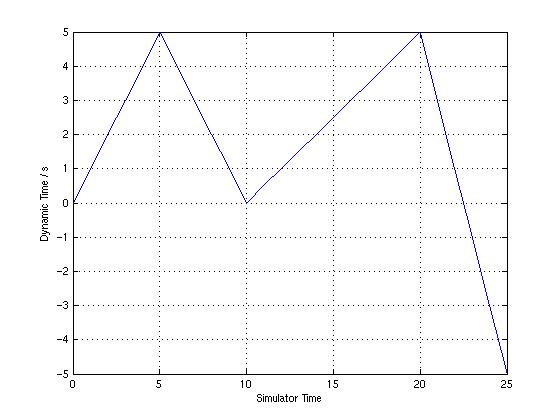
\includegraphics[width=3.2736in,height=2.85in]{figures/sim2_dyn.jpg}
\caption{Variation with Simulator Time of Dynamic Time.}
\end{center}
\end{figure}

\begin{figure}[htp]
\begin{center}
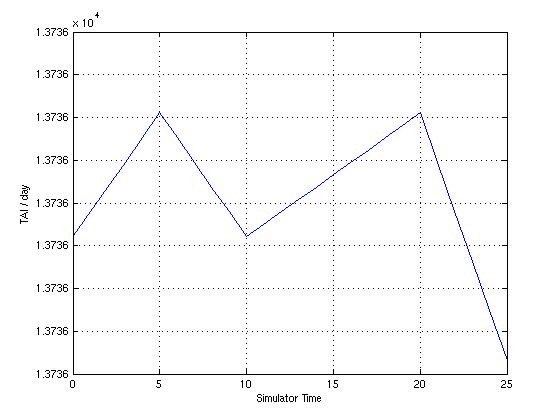
\includegraphics[width=3.2736in,height=2.85in]{figures/sim2_tai.jpg}
\caption{Variation with Simulator Time of TAI.}
\end{center}
\end{figure}

\begin{figure}[htp]
\begin{center}
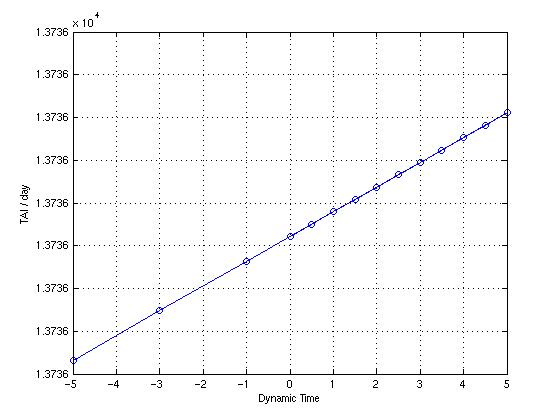
\includegraphics[width=3.2736in,height=2.85in]{figures/sim2_tai_dyn.jpg}
\caption{Variation with Dynamic Time of TAI.}
\end{center}
\end{figure}

\end{description}


\clearpage

\subsection{Verification of Presence of Derived Times and of the Initialization and Propagation Thereof}
\test{SIM\_5\_all\_inclusive/RUN\_UTC\_initialized}  \label{test:clockpresence}
\begin{description}
\item[Purpose:]\ \newline
To ensure that the clocks specified in requirement \ref{reqt:datatimerepresentation} are present and functioning.

\item[Requirement:]\ \newline
Satisfactory conclusion of this test satisfies requirement \ref{reqt:datatimerepresentation}.

Satisfactory conclusion of this test, together with \ref{test:UDEinitbyval} satisfies requirement \ref{reqt:timeinitializationUDE}.


\item[Procedure:]\ \newline
A simulation was developed that contained all clocks included in the release of \JEODid.

\item[Predictions:]\ \newline
All clocks will tick at their appropriate rates, with values consistent with each other.

\item[Results:]\ \newline
All clocks performed as expected.  Figure \ref{fig:sim5} shows the progression of the \textit{calendar\_second} and \textit{clock\_second} values during the simulation.

Some key observations from this plot:
\begin{itemize}
	\item After kicking down to 0 seconds (at the end of the minute), UTC holds for 1 second.  This is an effect of the leap second that was added there.
	\item MET1 is initialized in such a way that the respective values of UTC and MET1 are equivalent up to the addition of the leap second.  Since MET1 is scheduled to update from TAI (and therefore ticks with TAI), it will not have a leap second and will be offset from UTC for all time after the leap second.
	\item MET2 is scheduled to start with a negative value, and to hold during the middle of the simulation.
	\item UT1 advances a little behind UTC; after the leap second, it is a little ahead. 
	\item TDB is not shown; on this scale, it is an overlay of TT.
	\item Data is recorded every second; the last value recorded before the minute ticks over in UTC, UT1, and TT  is the last value in the range [59,60) s, which is not consistent between clocks (as expected).
	
\end{itemize}
  
\begin{figure}[htp]
\begin{center}
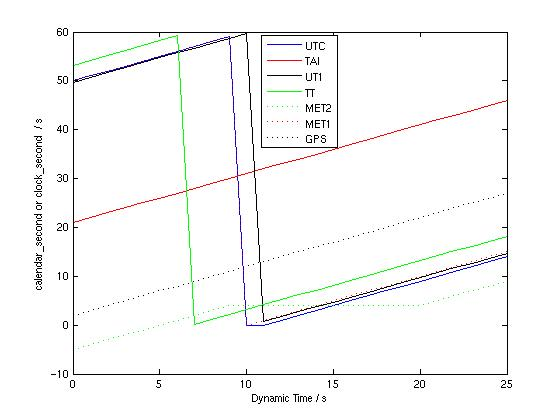
\includegraphics[width=3.2736in,height=2.85in]{figures/sim5_seconds.jpg}
\caption{Variation with Dynamic Time of Derived Times.}\label{fig:sim5}
\end{center}
\end{figure}
  
  

\end{description}














\clearpage




\subsubsection{Verification of TDB to TAI Conversion}

\test{SIM\_5\_all\_inclusive/RUN\_UTC\_initialized\_tdb}  \label{test:UDEinitbytdb}
\begin{description}
\item[Purpose:]\ \newline
To demonstrate that the newly added convert\_b\_to\_a() function correctly implements the
non-trivial conversion algorithm from TDB to TAI.

\item[Requirement:]\ \newline
Satisfactory conclusion of this test satisfies requirement \ref{reqt:timeinitializationrep},
providing the ability for time clocks to be converted to a different type in the reverse direction.

\item[Procedure:]\ \newline
The following entries in the input file were changed:
\begin{verbatim}
	LOG_CYCLE = 1.0
	execfile( "Log_data/log_rec_tdb.py" )

	jeod_time.utc.calendar_year = 2017
	jeod_time.utc.calendar_month = 10
	jeod_time.utc.calendar_day = 28
	jeod_time.utc.calendar_hour = 01.0
	jeod_time.utc.calendar_minute = 23.0
	jeod_time.utc.calendar_second = 45.0
\end{verbatim}
to change the initialization time to match the initialization time of a results comparison python script.
\begin{verbatim}
	jeod_time.tdb.initialize_from_name = "UTC"
\end{verbatim}
to
\begin{verbatim}
	jeod_time.tdb.initialize_from_name = "TAI"
\end{verbatim}
to change from a UTC-initialized simulation to a TAI-initialized simulation.
\begin{verbatim}
	trick.sim_services.exec_set_terminate_time(3600*2)
\end{verbatim}
to allow the simulation to run for two hours.

The following changes were made in the \textit{Log\_data} directory.

Create a new \textit{log\_rec.py} file named \textit{log\_rec\_tdb.py}. In this new file, remove all dr\_group.add\_variable("") lines of code, except for
\begin{verbatim}
	dr_group.add_variable( "jeod_time.tai.calendar_second")
	dr_group.add_variable( "jeod_time.tdb.calender_second")
\end{verbatim}
and change these lines to
\begin{verbatim}
	dr_group.add_variable( "jeod_time.tai.seconds")
	dr_group.add-variable( "jeod_time.tdb.seconds")
\end{verbatim}
This allows only the TAI and TDB variables to be recorded in seconds when the simulation runs.

\item[Predictions:]\ \newline
All clocks will tick at their appropriate rates, with values consistent with each other. Results produced by the simulation and the comparison script should be equal.

\item[Results:]\ \newline
All data consistent with expectations.

\end{description}


\subsection{Verification of Initialization by Derived Times}


\subsubsection{Verification of Initialization by Standard Time}


\test{SIM\_5\_all\_inclusive}  \label{test:STDinitbytype}
\begin{description}
\item[Purpose:]\ \newline
To demonstrate that changes to the identification of which type is the \textit{initializer}, coupled with associated changes to the initialization and update trees, and declaration of appropriate initial values, will result in the simulation being initialized in whichever time-type is desired. 

\item[Requirement:]\ \newline
Satisfactory conclusion of this test, and that of \ref{test:UDEinitbyval}, satisfies requirement \ref{reqt:timeinitializationrep}.

\item[Procedure:]\ \newline
The following entries in the input file were changed:
\begin{verbatim}
	time.manager_init.initializer = "UTC";
	time.utc.calendar_year = 1998;
  time.utc.calendar_month = 12; 
  time.utc.calendar_day = 31; 
  time.utc.calendar_hour = 23; 
  time.utc.calendar_minute = 59; 
  time.utc.calendar_second = 50.0;
\end{verbatim}
by replacing reference to UTC with reference to the desired class.

The initialization and update tree definitions were changed, e.g. from
\begin{verbatim}
  time.tai.initialize_from_name = "UTC";
\end{verbatim}
to 
\begin{verbatim}
  time.utc.initialize_from_name = "TAI";
\end{verbatim}
to change from a UTC-initialized simulation to a TAI-initialized simulation.
  
\item[Predictions:]\ \newline
All clocks should still initialize, but with different values because the initialization time has changed (it is numerically the same, but now on a different clock).
All clocks should progress as before.

\item[Results:]\ \newline
All data was consistent with expectations.

\end{description}




\test{SIM\_2\_dyn\_plus\_STD/initialize\_by\_value}\label{test:STDinitbyval}
\begin{description}
\item[Purpose:]\ \newline
To test the initialization routines, to ensure that a Standard Time can be initialized by a value expressed as a Truncated Julian Time value, a Modified Julian Time value, a Julian Day value, seconds since J2000, or days since J2000.

\item[Requirement:]\ \newline
Satisfactory conclusion of this test, together with test \ref{test:STDinitbycal}, and test \ref{test:UDEinitbyval} satisfy requirements \ref{reqt:timeinitializationbyformat} and \ref{reqt:formattimerepresentation}.

\item[Procedure:]\ \newline
The input file for the run identified as \textit{RUN\_initialize\_by\_value} contains several lines of options.  Each option was tested, one at a time, and the resulting data considered. 

For each option, the simulation was initialized to a value of 10,000 (units correspond to the option).  For each option, the output was plotted as a Truncated Julian Time representation.

\item[Predictions:]\ \newline
\begin{itemize}
	\item {Truncated Julian Time}
	
	The output should have a value of $10,000$ days.
	\item {Modified Julian Time}
	
	Modified Julian Time differs from truncated Julian Time by 40,000 days.  If Modified Julian Time = $10,000$ days, then Truncated Julian Time = $-30,000$ days.
	\item {Julian Time}
	
	Julian Time differs from Truncated Julian Time by 2,440,000.5 days.  If Julian Time = $10,000$ days, then Truncated Julian Time = $-2.4300005 \times 10^6 $ days.
	\item {seconds\_since\_epoch}
	
	The TAI epoch is set to J2000, corresponding to a Truncated Julian Time of $11544.4996275$ days in TAI.  $10,000$ seconds (or $0.11574$ days) after this point gives Truncated Julian Time = $11544.61536824074$ days.
	\item {days\_since\_epoch}
	
	10,000 days after the TAI epoch has a Truncated Julian Time of $21544.4996275$ days.
\end{itemize}

\item[Results:]\ \newline
  All values agreed with their predicted values.
\end{description}





\test{SIM\_2\_dyn\_plus\_STD/RUN\_initialize\_by\_calendar}  \label{test:STDinitbycal}
\begin{description}
\item[Purpose:]\ \newline
To test whether a Standard Time can be correctly initialized by a calendar representation.

\item[Requirement:]\ \newline
Satisfactory conclusion of this test, together with test \ref{test:STDinitbyval}, and test \ref{test:UDEinitbyval} satisfy requirement \ref{reqt:timeinitializationbyformat}.


\item[Procedure:]\ \newline
A simulation was created comprising Dynamic Time and TAI.  The initialization was set to a calendar value of 2005/12/31::23:59:50.0 TAI. 

\item[Predictions:]\ \newline
The calendar value should correspond to a Truncated Julian Time of 13735.9998842593

\item[Results:]\ \newline
The predicted value is correct.

\end{description}



\subsubsection{Verification of Initialization by User-defined-epoch Times}


\test{SIM\_5\_all\_inclusive/RUN\_UDE\_initialized}  \label{test:UDEinitbyval}
\begin{description}
\item[Purpose:]\ \newline
To test whether the \timeDesc\ can be initialized from a UDE time-type, using either an initial value, or a clock.

\item[Requirement:]\ \newline
Satisfactory conclusion of this test, together with test \ref{test:STDinitbycal}, and test \ref{test:STDinitbyval} satisfies requirement \ref{reqt:timeinitializationbyformat}.

Satisfactory conclusion of this test, together with test \ref{test:STDinitbytype}, satisfies requirement \ref{reqt:timeinitializationrep}.

Satisfactory conclusion of this test, together with test \ref{test:clockpresence}, satisfies requirement \ref{reqt:timeinitializationUDE}.




\item[Procedure:]\ \newline
In the all-inclusive simulation with an initialization by a UDE, there are two options for initializing the UDE (and hence the simulation).  One is by using the initial value of the UDE in \textit{seconds\_since\_epoch}, and the other by specifying a clock format (still representing time since epoch).  The same simulation was run with both options.

\item[Predictions:]\ \newline
The two runs should produce identical results, and the other time representations should generate data consistent with a simulation starting at 1998/12/31::23:59:50.0.

\item[Results:]\ \newline
The data are as expected.
\end{description}


\subsection{Verification of Data Over-rides}
\test{SIM\_4\_common\_usage/RUN\_JEOD1x\_compatible}  \label{test:overrides}
\begin{description}
\item[Purpose:]\ \newline
To ensure that the methods can be used for simulations set in the future for which data values are not included in the \JEODid\ release, and to demonstrate a method by which the \JEODid\ data output can be compared directly against that from previous releases.

\item[Requirement:]\ \newline
Satisfactory conclusion of this test satisfies requirement \ref{reqt:backwardcompatibility}.

\item[Procedure:]\ \newline
The flags \textit{true\_utc} and \textit{true\_ut1} were forced to false, effectively eliminating the capability of updating the offset values from the most recent data.  Instead, an offset between, say TAI and UTC, will be calculated initially, and that value will remain as a constant for the duration of the simulation.

\item[Predictions:]\ \newline
Running through the known instant of a leap second will produce no effect on UTC with the flags turned off.  The two UT1 values (with flag set to true and false) will be identical at the start of the simulation, and gradually diverge throughout the simulation.

\item[Results:]\ \newline
The data are as expected.
In the following figure legends, ``***-1'' refers to the JEOD1.x compatible
data, and ``***-2'' refers to the data obtained with the default settings in \JEODid.
Figure \ref{fig:sim4all} shows the relation between TAI, UTC, and UT1 at a time near the end of the simulation.  

Figure \ref{fig:sim4leap} represents a small part of figure \ref{fig:sim4all}, zoomed in. It shows the separation of the two UTC values at the point at which a leap second is encountered (Note that the leap second is added to the \JEODid\ version of UTC, and the JEOD1 version of UTC keeps ticking right through it).  

Figure \ref{fig:sim4ut1} represents a further zoom in, and shows the difference between the two UT1 times.

Finally, figure \ref{fig:sim4dut1} shows the difference between the two UT1 values clearly growing over time.  A similar plot differencing the two UTC values is not presented, it showed a flat line 0 preceding the leap second; thereafter, the difference was 1 second, except as the minutes ticked over, when it would jump to 59 seconds (because one time would tick over and go to zero while the other was still near 60).

\begin{figure}[htp]
\begin{center}
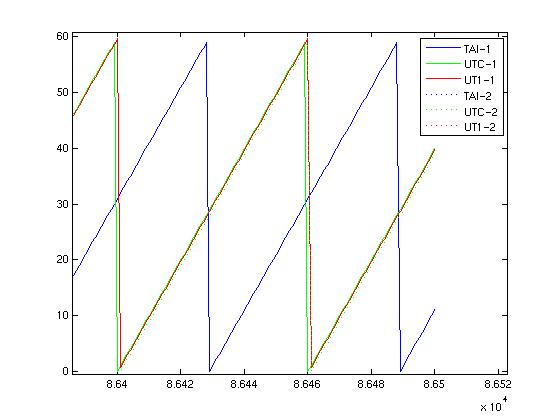
\includegraphics[width=3.2736in,height=2.85in]{figures/sim4_all.jpg}
\caption{Showing the relation between TAI, UTC, and UT1.}\label{fig:sim4all}
\end{center}
\end{figure}
\begin{figure}[htp]
\begin{center}
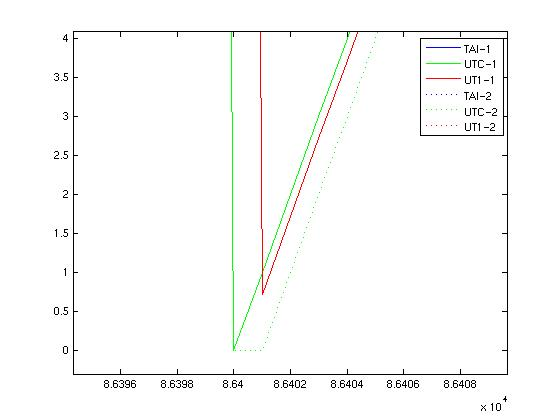
\includegraphics[width=3.2736in,height=2.85in]{figures/sim4_leap.jpg}
\caption{Values of UTC showing the addition of a leap second in the \JEODid-compatible version, but not in previous versions.}\label{fig:sim4leap}
\end{center}

\end{figure}
\begin{figure}[htp]
\begin{center}
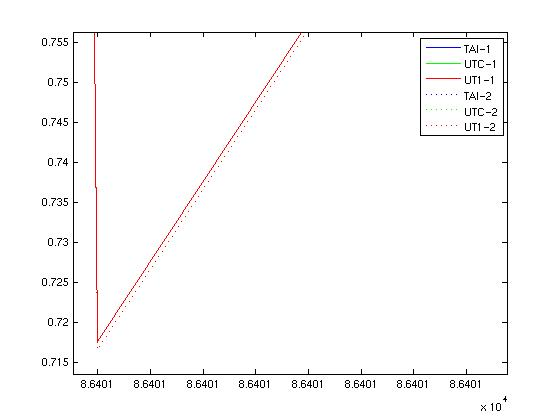
\includegraphics[width=3.2736in,height=2.85in]{figures/sim4_ut1_end.jpg}
\caption{Values of UT1 showing the difference between performing regular updates and using a fixed data-file override value.  This difference is after approximately 1 day of Dynamic Time.}\label{fig:sim4ut1}
\end{center}

\end{figure}
\begin{figure}[htp]
\begin{center}
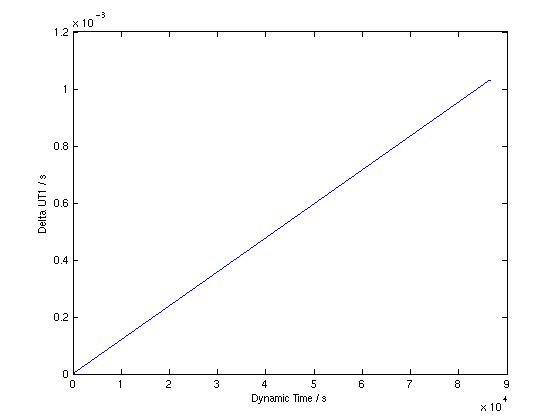
\includegraphics[width=3.2736in,height=2.85in]{figures/sim4_deltaut1.jpg}
\caption{The difference,over a period of 1 day, between the values of UT1 using a regular update, versus using a fixed data-file override value.}\label{fig:sim4dut1}
\end{center}
\end{figure}
\end{description}

\clearpage

\subsection{Verification of Extension Capabilities}
\test{SIM\_6\_extension}  \label{test:sim6}
\begin{description}
\item[Purpose:]\ \newline
To ensure that new clocks and converters can be added without altering the
existing code-base.

\item[Requirement:]\ \newline
Satisfactory conclusion of this test satisfies requirement
\ref{reqt:extensibility}.

\item[Procedure:]\ \newline
A new clock and accompanying converter were added to the simulation, as
described in the \textref{User Guide}{sec:User_Extension}.

\item[Predictions:]\ \newline
The time would evolve as Dynamic Time progresses.

\item[Results:]\ \newline
The data are as expected.
\end{description}


%\section{Validation}
%%%%%%%%%%%%%%%%%%%%%%%%%%%%%%%%%%%%%%%%%%%%%%%%%%%%%%%%%%%%%%%%%%%%%%%%%%%%%%%%
%
% Purpose:  Validation part of V&V for the time model
%
% 
%
%%%%%%%%%%%%%%%%%%%%%%%%%%%%%%%%%%%%%%%%%%%%%%%%%%%%%%%%%%%%%%%%%%%%%%%%%%%%%%%%

\section{Validation}

%%% code imported from old template structure

The overall functionality of the \timeDesc\ has been validated using 
respectable conversion tools, mostly
provided by the United States' Naval Observatoy, to validate that our clocks are
internally consistent, and that the decimal representation of time is consistent
with the calendar/clock representation of time.  In no test was a discrepancy
found within the level of precision of those conversion tools.

Output has also been validated against output from earlier releases of JEOD; it
has been demonstrated that for a JEOD 1.x-compatible simulation, flags can be 
set
to provide equivalent data.  However, it has been found that the new 
implementation 
is closer to clock standards than the old implementation; the old implementation
should be used in very limited circumstances.

The time-reversal feature of the \timeDesc\ has been validated internally, by 
comparing state data from forward and reverse simulations.

\test{SIM\_7\_time\_reversal}\label{test:timereversal}
\begin{description}
\item[Purpose:] \ \newline
To evaluate the capability of the \JEODid\ models to handle time reversal 
simulations.
\item[Requirements:] \ \newline
Satisfactory conclusion of this test satisfies requirement 
\ref{reqt:physicaltime}.
\item[Procedure:]\ \newline
A selection of the simulation runs from the top-level verification simulation, 
SIM\_dyncomp were copied.  These simulations were set to run forward for 60,000 
seconds, at which time the time would reverse, and run backward for 60,000 
seconds.
\item[Predictions:]
The final state should be identical to the initial state.  While this is not 
possible to achieve by any means other than a statistical fluke (due to 
numerical rounding), the extent to which the two states differ gives 
significant data on how well the time reversal functions.
\item[Results:]\ \newline
For all tests, the same technique was used to graph the data, with all graphs 
showing the difference between the state in the forward and reverse parts of 
the simulation.  

On the graph, time t=0 corresponds to the turnaround at simulation time = 
60,000 seconds; there is no difference in the state at this time.  Graphical 
time t= 60,000 seconds corresponds to the difference between the state at 
simulation time t=0 (in the forward component of the simulation), and the state 
at simulation time t= 120,000 seconds (in the reverse component of the 
simulation).

The following tests were used:

{\bf RUN\_1:}
This run tests simple propagation in a spherical gravity field. 

The position diverges by microns over the 120,000 seconds of the simulation 
(see figure \ref{fig:sim71pos}).

The velocity diverged by nano-meters per second (see figure \ref{fig:sim71vel}).

\begin{figure}[htp]
\begin{center}
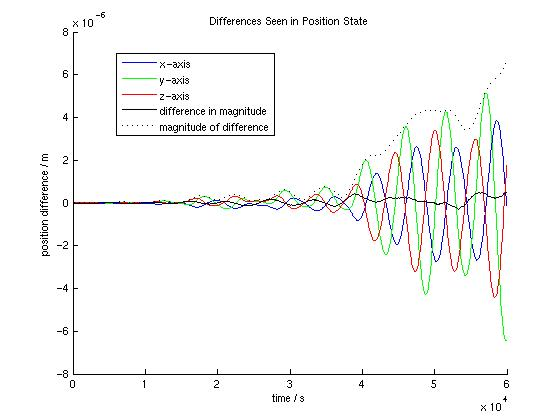
\includegraphics[width=3.2736in,height=2.85in]{figures/run1pos.jpg}
\caption{The difference in the position state for RUN\_1.}
\label{fig:sim71pos}
\end{center}
\end{figure}

\begin{figure}[htp]
\begin{center}
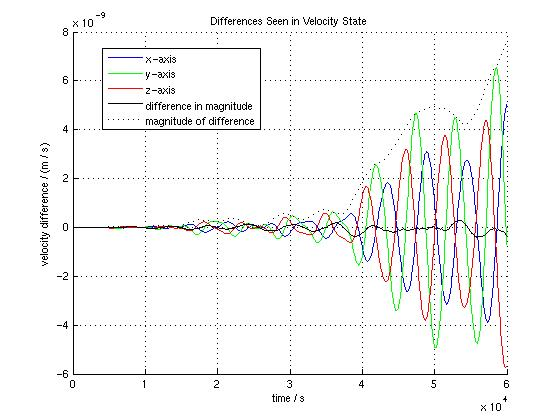
\includegraphics[width=3.2736in,height=2.85in]{figures/run1vel.jpg}
\caption{The difference in the velocity state for RUN\_1.}
\label{fig:sim71vel}
\end{center}
\end{figure}
 
\clearpage
{\bf RUN\_3A}
This run tests simple propagation in a nonspherical, 4x4 gravity field. 

The position diverges by centi-meters over the 120,000 seconds of the 
simulation (see figure \ref{fig:sim73apos}).

The velocity diverged by $O(10^{-5})$ meters per second (see figure 
\ref{fig:sim73avel}).


\begin{figure}[htp]
\begin{center}
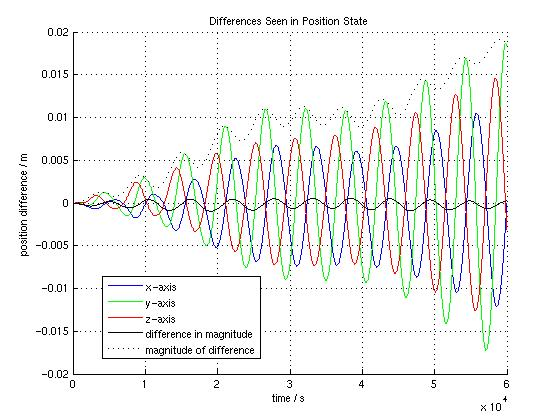
\includegraphics[width=3.2736in,height=2.85in]{figures/run3apos.jpg}
\caption{The difference in the position state for RUN\_3A.}
\label{fig:sim73apos}
\end{center}
\end{figure}

\begin{figure}[htp]
\begin{center}
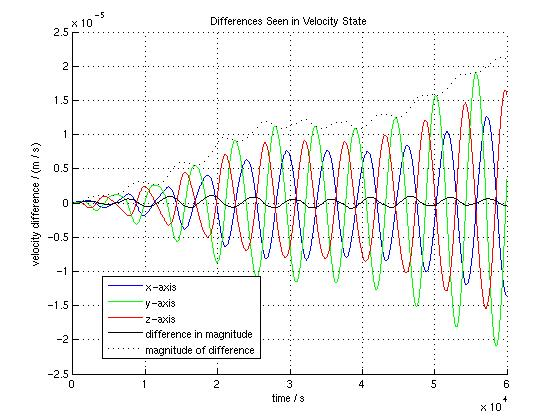
\includegraphics[width=3.2736in,height=2.85in]{figures/run3avel.jpg}
\caption{The difference in the velocity state for RUN\_3A.}
\label{fig:sim73avel}
\end{center}
\end{figure}



\clearpage
{\bf RUN\_3B}
This run tests simple propagation in a nonspherical, 8x8 gravity field. 

The position diverges by centimeters over the 120,000 seconds of the simulation 
(see figure \ref{fig:sim73bpos}).

The velocity diverged by $O(10^{-5})$ meters per second (see figure 
\ref{fig:sim73bvel}).


Because these data were significantly worse than the other simulations, we 
tried changing the rate at which the RNP matrix was being updated from once 
every 60 seconds to updates at 32 Hz, the same as the dynamic rate.  The 
rationale was demonstrated to have some validity, although the divergences in 
the enhanced state were still relatively large (see figures 
\ref{fig:sim73bhispdpos} and \ref{fig:sim73bhispdvel} for the enhanced 
simulation data).



\begin{figure}[htp]
\begin{center}
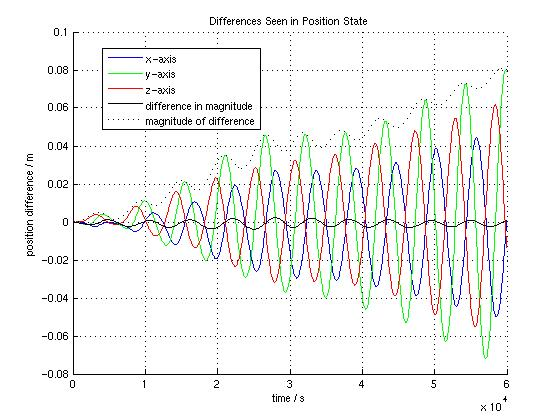
\includegraphics[width=3.2736in,height=2.85in]{figures/run3bpos.jpg}
\caption{The difference in the position state for RUN\_3B.}
\label{fig:sim73bpos}
\end{center}
\end{figure}

\begin{figure}[htp]
\begin{center}
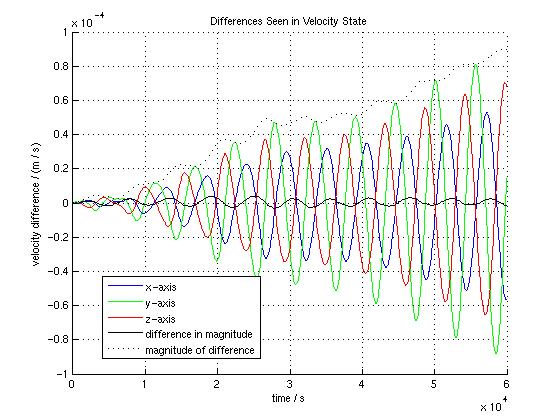
\includegraphics[width=3.2736in,height=2.85in]{figures/run3bvel.jpg}
\caption{The difference in the velocity state for RUN\_3B.}
\label{fig:sim73bvel}
\end{center}
\end{figure}

\begin{figure}[htp]
\begin{center}
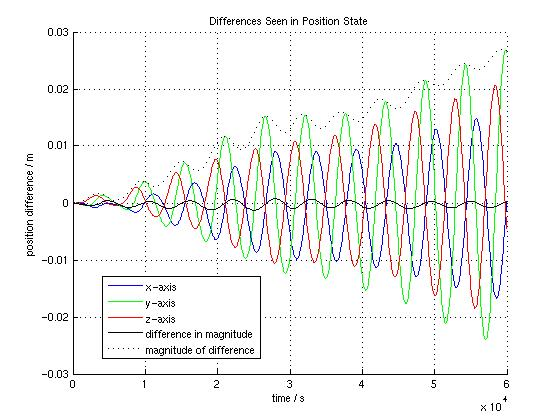
\includegraphics[width=3.2736in,height=2.85in]{figures/run_3bhispdpos.jpg}
\caption{The difference in the position state for RUN\_3B.}
\label{fig:sim73bhispdpos}
\end{center}
\end{figure}

\begin{figure}[htp]
\begin{center}
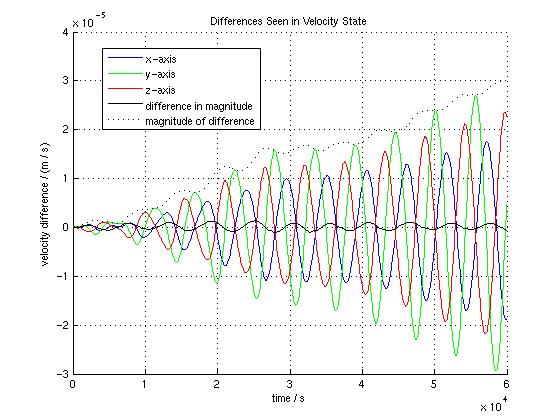
\includegraphics[width=3.2736in,height=2.85in]{figures/run_3bhispdvel.jpg}
\caption{The difference in the velocity state for RUN\_3B.}
\label{fig:sim73bhispdvel}
\end{center}
\end{figure}

\clearpage
{\bf RUN\_4}
This run tests propagation in a spherical gravitational field with 3rd body 
perturbations.

The position diverges by $O(10^{-5})$ meters over the 120,000 seconds of the
simulation (see figure \ref{fig:sim74pos}).

The velocity diverged by $O(10^{-8})$ meters per second (see figure
\ref{fig:sim74vel}).

\begin{figure}[htp]
\begin{center}
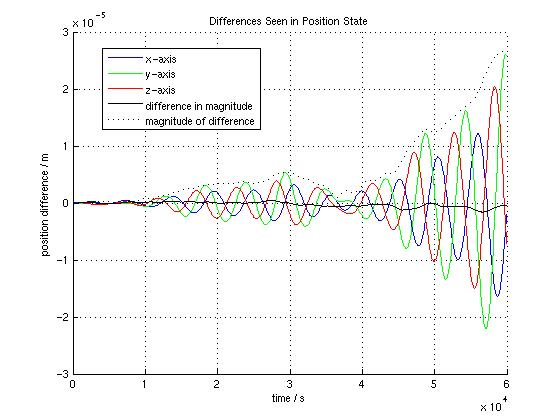
\includegraphics[width=3.2736in,height=2.85in]{figures/run4pos.jpg}
\caption{The difference in the position state for RUN\_4.}
\label{fig:sim74pos}
\end{center}
\end{figure}

\begin{figure}[htp]
\begin{center}
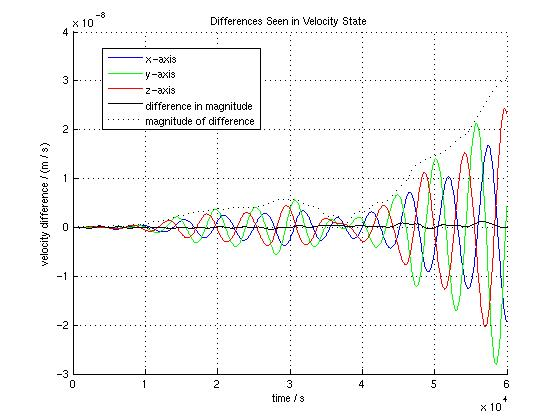
\includegraphics[width=3.2736in,height=2.85in]{figures/run4vel.jpg}
\caption{The difference in the velocity state for RUN\_4.}
\label{fig:sim74vel}
\end{center}
\end{figure}


\clearpage
{\bf RUN\_6A}
This run tests propagation in a spherical gravitational field with aerodynamic 
drag effects included.

The position diverges by $O(10^{-4})$ meters over the 120,000 seconds of the 
simulation (see figure \ref{fig:sim76apos}).

The velocity diverged by $O(10^{-7})$ meters per second (see figure 
\ref{fig:sim76avel}).

\begin{figure}[htp]
\begin{center}
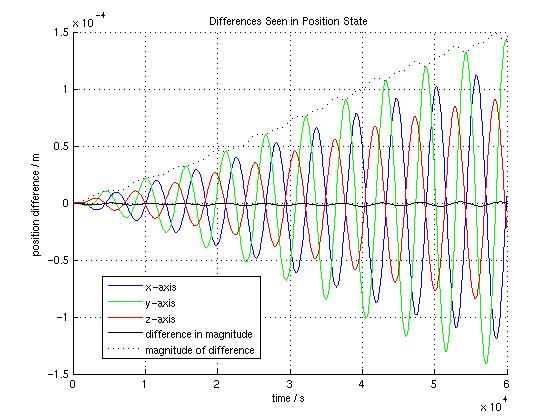
\includegraphics[width=3.2736in,height=2.85in]{figures/run6apos.jpg}
\caption{The difference in the position state for RUN\_6A.}
\label{fig:sim76apos}
\end{center}
\end{figure}

\begin{figure}[htp]
\begin{center}
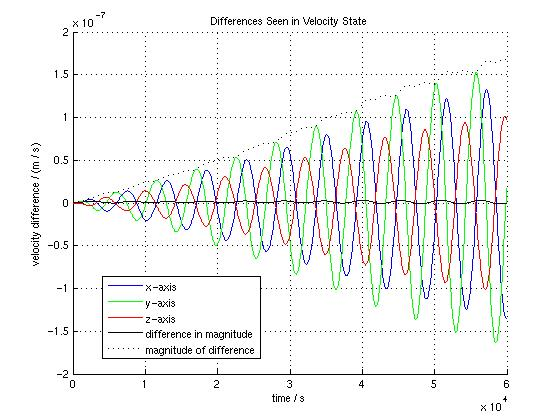
\includegraphics[width=3.2736in,height=2.85in]{figures/run6avel.jpg}
\caption{The difference in the velocity state for RUN\_6A.}
\label{fig:sim76avel}
\end{center}
\end{figure}

\clearpage
{\bf RUN\_8B}
This run tests propagation in a spherical gravitational field with the 
rotational state also available.  Only rotational data is provided here; the 
translational state is equivalent to that in RUN\_1.  RUN\_8B was chosen 
because it starts with a non-zero rotational state.

The quaternion values diverge by $O(10^{-14})$ over the 120,000 seconds of the 
simulation (see figure \ref{fig:sim78bpos}).

The angular velocity diverged by $O(10^{-14})$ radians per second (see figure 
\ref{fig:sim78bvel}).

\begin{figure}[htp]
\begin{center}
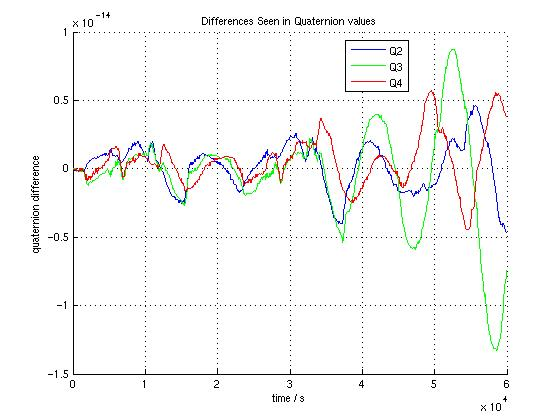
\includegraphics[width=3.2736in,height=2.85in]{figures/run8bpos.jpg}
\caption{The difference in the quaternion values for RUN\_8B.}
\label{fig:sim78bpos}
\end{center}
\end{figure}

\begin{figure}[htp]
\begin{center}
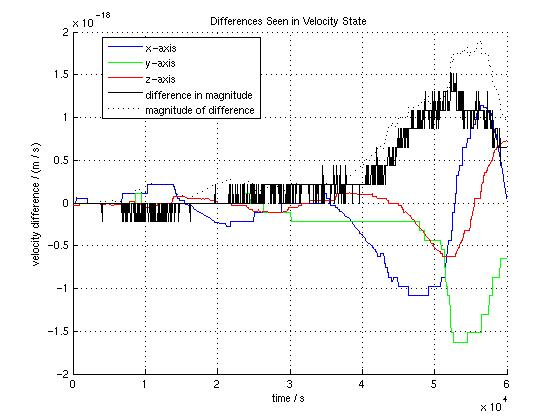
\includegraphics[width=3.2736in,height=2.85in]{figures/run8bvel.jpg}
\caption{The difference in the angular velocity state for RUN\_8B.}
\label{fig:sim78bvel}
\end{center}
\end{figure}

\clearpage
{\bf RUN\_9D}
This run tests propagation in a spherical gravitational field with rotational 
state and external torques and forces.  For this simulation, an external force 
and torque was applied between times t= 10,000 seconds and t = 20,000 seconds 
and then again between times t=100,000 seconds and t = 110,000 seconds to 
maintain the symmetry for the forward and reverse components.

The effect of the forces and torques on the state at the times for which they 
are active can be seen in figures \ref{fig:sim79dposoverall} and 
\ref{fig:sim79daveloverall}.

The position diverges by $O(10^{-7})$ meters over the 120,000 seconds of the 
simulation (see figure \ref{fig:sim79dpos}).

The velocity diverged by $O(10^{-10})$ meters per second (see figure 
\ref{fig:sim79dvel}).

The quaternion values diverge by $O(10^{-14})$ over the 120,000 seconds of the 
simulation (see figure \ref{fig:sim79dquat}).

The angular velocity diverged by $O(10^{-19})$ radians per second, at the limit 
of resolution (see figure \ref{fig:sim79davel}).


\begin{figure}[htp]
\begin{center}
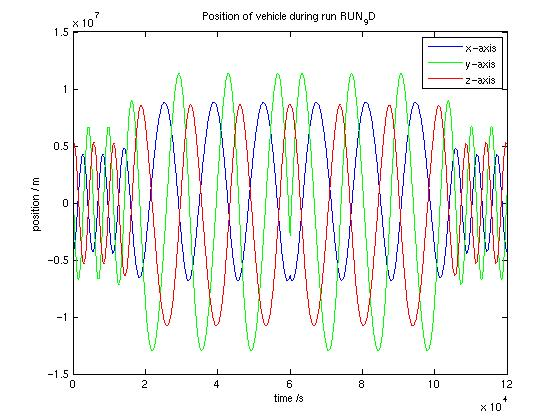
\includegraphics[width=3.2736in,height=2.85in]{figures/run_9dposoverall.jpg}
\caption{The position state for RUN\_9D.}
\label{fig:sim79dposoverall}
\end{center}
\end{figure}

\begin{figure}[htp]
\begin{center}
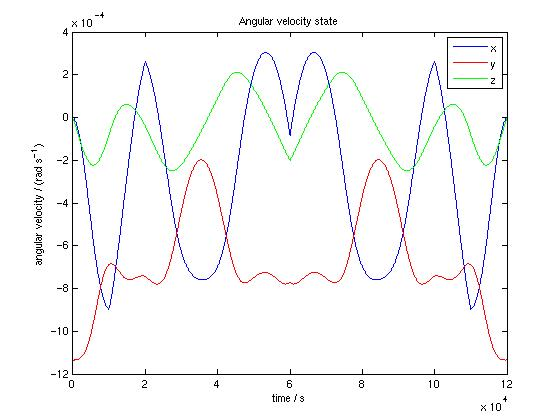
\includegraphics[width=3.2736in,height=2.85in]{figures/run_9daveloverall.jpg}
\caption{The angular velocity state for RUN\_9D.}
\label{fig:sim79daveloverall}
\end{center}
\end{figure}

\begin{figure}[htp]
\begin{center}
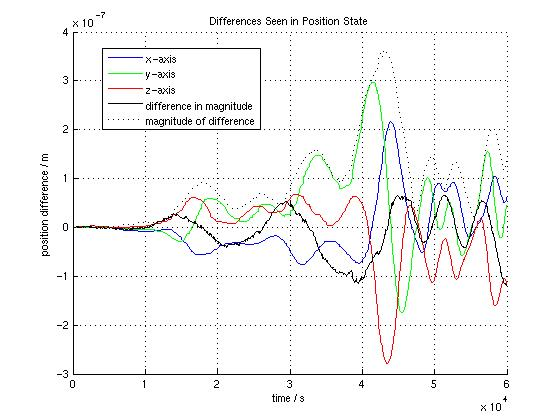
\includegraphics[width=3.2736in,height=2.85in]{figures/run_9dpos.jpg}
\caption{The difference in the position state for RUN\_9D.}
\label{fig:sim79dpos}
\end{center}
\end{figure}

\begin{figure}[htp]
\begin{center}
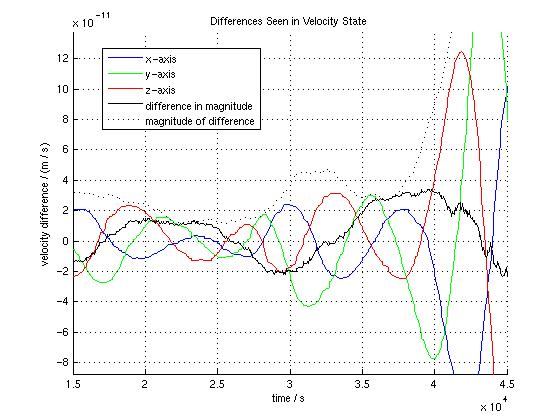
\includegraphics[width=3.2736in,height=2.85in]{figures/run_9dvel.jpg}
\caption{The difference in the velocity state for RUN\_9D.}
\label{fig:sim79dvel}
\end{center}
\end{figure}

\begin{figure}[htp]
\begin{center}
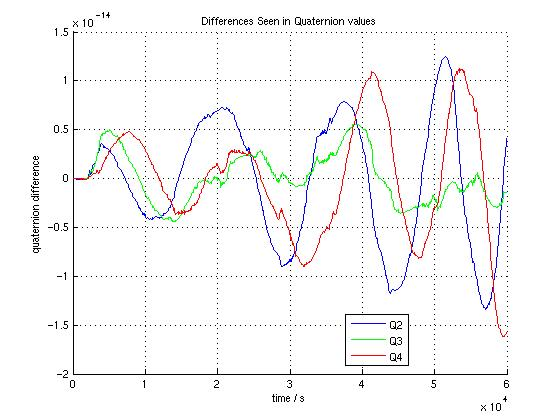
\includegraphics[width=3.2736in,height=2.85in]{figures/run_9dquat.jpg}
\caption{The difference in the quaternion values for RUN\_9D.}
\label{fig:sim79dquat}
\end{center}
\end{figure}

\begin{figure}[htp]
\begin{center}
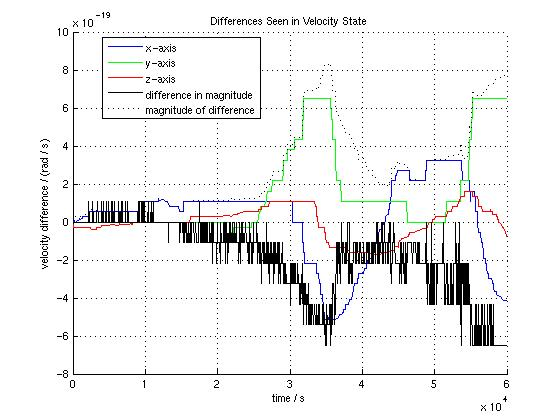
\includegraphics[width=3.2736in,height=2.85in]{figures/run_9davel.jpg}
\caption{The difference in the angular velocity state for RUN\_9D.}
\label{fig:sim79davel}
\end{center}
\end{figure}


\clearpage
{\bf RUN\_10A}
This final run tests propagation in a spherical gravitational field with 
gravity gradient torque present.

The position diverges by $O(10^{-6})$ meters over the 120,000 seconds of the 
simulation (see figure \ref{fig:sim710apos}).

The velocity diverged by $O(10^{-9})$ meters per second (see figure 
\ref{fig:sim710avel}).

The quaternion values diverge by $O(10^{-13})$ over the 120,000 seconds of the 
simulation (see figure \ref{fig:sim710aquat}).

The angular velocity diverged by $O(10^{-16})$ radians per second, at the limit 
of resolution (see figure \ref{fig:sim710aavel}).


\begin{figure}[htp]
\begin{center}
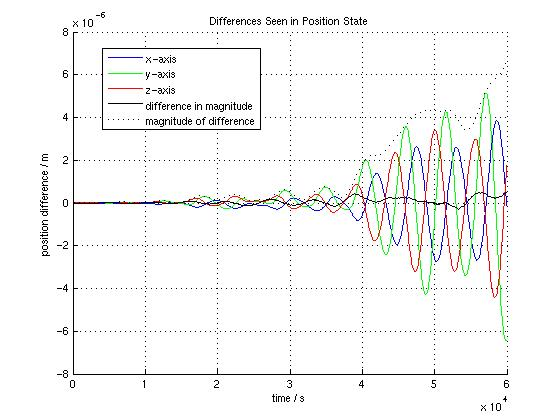
\includegraphics[width=3.2736in,height=2.85in]{figures/run_10apos.jpg}
\caption{The difference in the position state for RUN\_10A.}
\label{fig:sim710apos}
\end{center}
\end{figure}

\begin{figure}[htp]
\begin{center}
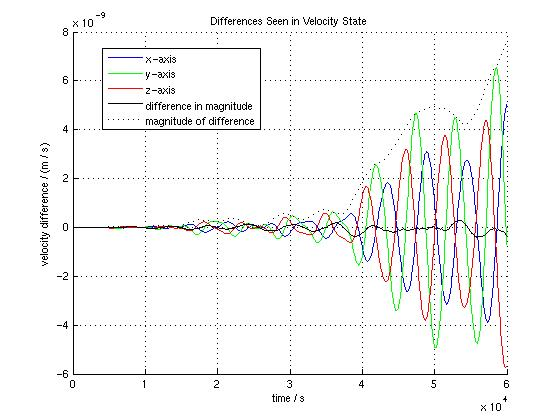
\includegraphics[width=3.2736in,height=2.85in]{figures/run_10avel.jpg}
\caption{The difference in the velocity state for RUN\_10A.}
\label{fig:sim710avel}
\end{center}
\end{figure}

\begin{figure}[htp]
\begin{center}
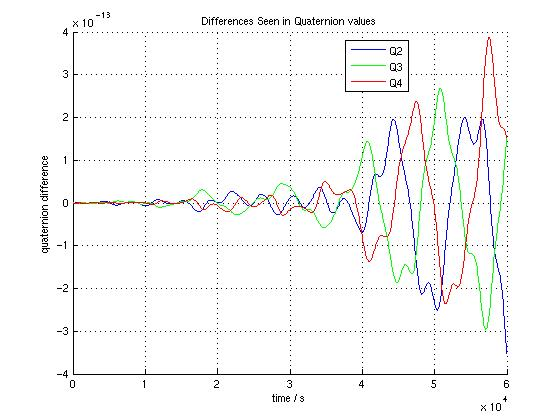
\includegraphics[width=3.2736in,height=2.85in]{figures/run_10aquat.jpg}
\caption{The difference in the quaternion values for RUN\_10A.}
\label{fig:sim710aquat}
\end{center}
\end{figure}

\begin{figure}[htp]
\begin{center}
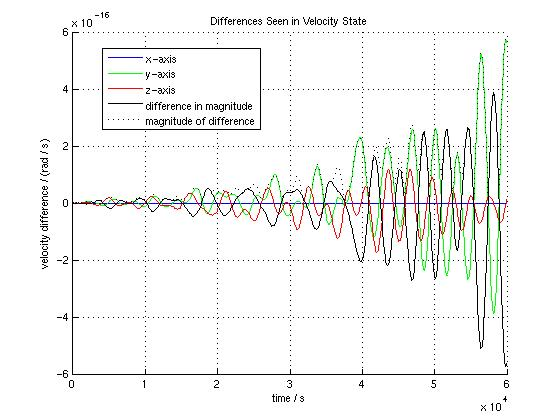
\includegraphics[width=3.2736in,height=2.85in]{figures/run_10aangvel.jpg}
\caption{The difference in the angular velocity state for RUN\_10A.}
\label{fig:sim710aavel}
\end{center}
\end{figure}

\end{description}


\section{Metrics}
\subsection{Code Metrics}

Table~\ref{tab:coarse_metrics} presents coarse metrics on the
source files that comprise the model.

\input{coarse_metrics}

Table~\ref{tab:metrix_metrics} presents the extended cyclomatic
complexity
(ECC) of the methods defined in the model.
\input{metrix_metrics}



%%%%%%%%%%%%%%%%%%%%%%%%%%%%%%%%%%%%%%%%%%%%%%%%%%%%%%%%%%%%%%%%%%%%%%%%%
% Bibliography
%%%%%%%%%%%%%%%%%%%%%%%%%%%%%%%%%%%%%%%%%%%%%%%%%%%%%%%%%%%%%%%%%%%%%%%%%
\newpage
\pdfbookmark{Bibliography}{bibliography}
\bibliography{dynenv,time}
\bibliographystyle{plain}

%\pagebreak
%\appendix

\end{document}
